%% LyX 2.5.2 created this file.  For more info, see https://www.lyx.org/.
%% Do not edit unless you really know what you are doing.
\documentclass[journal,article,submit,moreauthors]{Definitions/mdpi}
\usepackage{textcomp}
\usepackage[utf8]{inputenc}
\synctex=-1
\usepackage{longtable}
\usepackage{float}
\usepackage{url}
\usepackage{pdflscape}
\usepackage{amstext}
\usepackage{graphicx}

\makeatletter

%%%%%%%%%%%%%%%%%%%%%%%%%%%%%% LyX specific LaTeX commands.

\Title{Enhancing Rule Construction in Grammatical Evolution with Advanced
Crossover Techniques}

\Author{\textsubscript{\textsuperscript{}}Ioannis G. Tsoulos$^{1*}$, George
Georgoulas$^{2}$ and Vasileios Charilogis$^{3}$}


\address{$^{1}\quad$Department of Informatics and Telecommunications. University
of Ioannina, Greece; itsoulos@uoi.gr\\
$^{2}$\quad{}Department of Mechanical Engineering and Aeronautics,
University of Patras, Panepistimioupoli Patron, Rio 26504, Greece;
georgoul@gmail.com\\
$^{3}\quad$Department of Informatics and Telecommunications. University
of Ioannina, Greece; charilog@uoi.gr}


\corres{Correspondence: itsoulos@uoi.gr}


\abstract{Many real-world problems can be formulated as classification tasks
in machine learning and addressed using a wide range of advanced algorithms
developed for this purpose. Among these approaches, methods based
on Grammatical Evolution (GE) can also be employed, such as GenClass,
a technique designed to automatically construct classification rules.
Although GenClass has been successfully applied to a variety of classification
problems, its evolutionary search process may suffer from limitations
such as entrapment in local minima of the error function and premature
convergence, which can prevent the method from discovering high-quality
classification rules. The present work proposes an enhanced version
of GenClass through the introduction of advanced crossover techniques
operating on the integer-valued chromosomes employed by the method,
with the aim of improving the evolutionary search process and reducing
classification error. The proposed crossover operators follow two
different strategies. Some of them are purely stochastic, introducing
greater diversity into the evolutionary search, whereas others exploit
information already generated during the Grammatical Evolution process
to perform targeted exchanges of genetic material between chromosomes.
In this way, the latter operators attempt to guide the evolutionary
search toward more promising regions of the search space while preserving
useful information discovered during previous generations. The proposed
techniques were evaluated on a diverse collection of real-world classification
datasets, including several problems characterized by a large number
of patterns and/or a large number of classes. The experimental results
demonstrate that the Standard crossover strategy provides the most
consistent improvement over the original GenClass method, reducing
the average classification error from 16.13\% to 13.42\% across 31
classification datasets. This improvement remains statistically significant
after excluding four related EEG-derived datasets and applying a correction
for multiple comparisons. Among the three investigated crossover strategies,
the simplest approach, Standard, achieved the lowest average classification
error, whereas the more elaborate grammar-guided Targeted and TargetedWorst
variants did not provide further improvements.}


\keyword{Grammatical Evolution; Classification; Crossover Operators; Evolutionary
Algorithms; Machine Learning.}

\DeclareTextSymbolDefault{\textquotedbl}{T1}
%% Because html converters don't know tabularnewline
\providecommand{\tabularnewline}{\\}

%%%%%%%%%%%%%%%%%%%%%%%%%%%%%% User specified LaTeX commands.
%  LaTeX support: latex@mdpi.com
%  For support, please attach all files needed for compiling as well as the log file, and specify your operating system, LaTeX version, and LaTeX editor.
%=================================================================
%\documentclass[journal,article,submit,moreauthors,unicode]{Definitions/mdpi} % For some letters Palatino lacks
%\documentclass[preprints,article,submit,moreauthors]{Definitions/mdpi} 
%\documentclass[preprints,article,submit,moreauthors,unicode]{Definitions/mdpi} 
% For posting an early version of this manuscript as a preprint, you may use "preprints" as the journal. Changing "submit" to "accept" before posting will remove line numbers.

%--------------------
% Class Options:
%--------------------
%----------
% journal
%----------
% Choose between the following MDPI journals:

% Below journals will use APA reference format:
% admsci, aieduc, behavsci, businesses, econometrics, economies, education, ejihpe, famsci, fclam, games, humans, ijcs, ijfs, investment, joi, jintelligence, journalmedia, jrfm, jsam, languages, opermanag, peacestud, pmh, psycholint, publications, sciedu, tourismhosp, xmanagement, youth

% Below journals will use Chicago reference format:
% arts, genealogy, histories, humanities, laws, literature, religions, risks, socsci

% Below journals will use ACS reference format:
% accountaudit, acn, acoustics, actuators, addictions, addictprev, adhesives, adolescents, aee, aerobiology, aeronautics, aerospace, agriculture, agriengineering, agrochemicals, agronomy, ai, aiagents, aichem, aieng, aimater, aimed, aipa, air, aisens, aisoc, algorithms, allergies, alloys, amh, analog, analytica, analytics, anatomia, anesthres, animals, antibiotics, antibodies, antioxidants, applbiosci, appliedchem, appliedmath, appliedphys, applmech, applmicrobiol, applnano, applsci, aps, aquacj, archaeolstud, architecture, arm, arthropoda, asc, asd, asi, astronautics, astronomy, atmosphere, atoms, audiolres, automation, axioms, bacteria, batteries, bcrc, bdcc, beverages, bioactives, biochem, bioengineering, biologics, biology, biomass, biomechanics, biomed, biomedicines, biomedinformatics, biomimetics, biomolecules, biophysica, bioresourbioprod, biosensors, biosphere, biotech, birds, blockchains, bloods, blsf, brainsci, breath, buildings, cancers, carbon, cardio, cardiogenetics, cardiovascmed, catalysts, cells, ceramics, challenges, chemeco, chemengineering, chemistry, chemosensors, chemproc, children, chips, cimb, civileng, cleantechnol, climate, clinbioenerg, clinpract, clockssleep, cmd, cmtr, coasts, coatings, colloids, colorants, commodities, complexities, complications, compounds, computation, computers, condensedmatter, conservation, constrmater, cosmetics, covid, crops, cryo, cryptography, crystals, csmf, ctn, culture, curroncol, cyber, dairy, data, ddc, dentistry, dermato, dermatopathology, designs, devices, dgg, dhi, diabetology, diagnostics, dietetics, digital, disabilities, diseases, diversity, dna, drones, drugreact, drylands, dynamics, earth, ebj, ece, ecm, ecologies, edm, eesp, electricity, electrochem, electronicmat, electronics, embodiedintell, encyclopedia, endocrines, energies, eng, engproc, entomology, entropy, environments, environremediat, enzymology, epidemiologia, epigenomes, epilepsy, esa, est, fermentation, fibers, fintech, fire, fishes, fluids, foodeng, foods, forecasting, forensicsci, forests, fossstud, foundations, fractalfract, freshwater, fuels, future, futureinternet, futurepharmacol, futurephys, futuretransp, galaxies, gases, gastroent, gastrointestdisord, gastronomy, gels, genes, geochem, geographies, geohazards, geomatics, geometry, geosciences, geotechnics, geriatrics, germs, glacies, grainsci, grasses, green, greenhealth, gucdd, gynecolcancer, hardware, hazardousmatters, healthcare, healthcmater, hearts, hemato, hematolrep, hep, heritage, higheredu, highthroughput, horticulturae, hospitals, humanoids, hydrobiology, hydrogen, hydrology, hydrometeorology, hydropower, hygiene, idr, iic, ijem, ijerph, ijgi, ijmd, ijms, ijns, ijom, ijp, ijpb, ijt, ijtm, ijtpp, ijtst, ime, immuno, industries, inflammj, informatics, information, infrastructures, inorganics, insects, instruments, inventions, iot, iron, j, jaestheticmed, jal, japma, jcdd, jcm, jcp, jcrm, jcs, jcto, jdad, jdb, jdcp, jdream, jemr, jeta, jfb, jfmk, jfth, jgbg, jgg, jimaging, jlpea, jmahp, jmmp, jmms, jmp, jmse, jne, jnt, jof, joitmc, joma, jop, joptm, jor, jox, jpbi, jphytomed, jpm, jsan, jtaer, jvd, jzbg, kidneydial, kinasesphosphatases, knowledge, labmed, laboratories, lam, land, langtechnol, lasers, legumes, life, lights, limnolrev, lipidology, liquids, livers, logics, logistics, lubricants, lymphatics, machines, macromol, magnetism, magnetochemistry, make, marinedrugs, maritime, materials, materproc, mathematics, mca, mcb, measurements, meb, medicina, medicines, medsci, membranes, merits, metabolites, metals, metamaterialsadv, meteorology, methane, metrics, metrology, micro, microarrays, microbiolres, microelectronics, micromachines, microorganisms, microplastics, microwave, minerals, mining, mmphys, modelling, molbank, molecules, mollusca, mps, msf, mti, multimedia, muscles, mutation, nanoenergyadv, nanomanufacturing, nanomaterials, ncrna, ndt, network, neuroglia, neuroimaging, neurolint, neurosci, nitrogen, notspecified, nursrep, nutraceuticals, nutrients, obesities, occuphealth, oceans, ohbm, onco, optics, optoelectronics, oral, organics, organoids, osteology, oxygen, pandemics, parasites, parasitologia, particles, pathogens, pathophysiology, pediatrrep, pets, pharmaceuticals, pharmaceutics, pharmacoepidemiology, pharmacy, phc, philosophies, photochem, photonics, photovoltaics, phycology, physchem, physics, physiologia, plants, plasma, platforms, pnr, pollutants, polymers, polysaccharides, populations, poultry, powders, precision, precisoncol, preprints, prevhealthc, proceedings, processes, prosthesis, proteomes, psf, psychiatryint, psychoactives, purification, quantumrep, quaternary, qubs, radiation, rareearths, rdt, reactions, realestate, receptors, recycling, regeneration, remotesensing, reports, reprodmed, resources, rheumato, rjpm, robotics, rsee, ruminants, safety, sanpp, sca, sci, scipharm, sclerosis, seeds, sensors, senssyst, separations, sexes, shi, signals, sinusitis, siuj, skins, smartcities, smartfish, smartgrids, sna, societies, software, soilsystems, solar, solids, spectroscj, sports, standards, stats, std, stratsediment, stresses, strokerep, superintelligence, surfaces, surgeries, susagric, suschem, sustainability, sustainfoods, sustainpackag, symmetry, synbio, systems, tae, targets, taxonomy, technologies, telecom, test, textiles, thalassrep, therapeutics, thermo, timespace, tomography, toxics, toxins, tph, transplantology, transportation, traumacare, traumas, tri, tropicalmed, universe, urbansci, uro, vaccines, vehicles, venereology, vetsci, vibration, virtualworlds, viruses, vision, waste, water, welding, wem, wevj, wild, wind, women, world, zoonoticdis

%---------
% article
%---------
% The default type of manuscript is "article", but can be replaced by: 
% abstract, addendum, article, benchmark, book, bookreview, briefcommunication, briefreport, casereport, changes, clinicopathologicalchallenge, comment, commentary, communication, conceptpaper, conferenceproceedings, correction, conferencereport, creative, datadescriptor, discussion, entry, expressionofconcern, extendedabstract, editorial, essay, erratum, fieldguide, hypothesis, interestingimages, letter, meetingreport, monograph, newbookreceived, obituary, opinion, proceedingpaper, projectreport, reply, retraction, review, perspective, protocol, shortnote, studyprotocol, supfile, systematicreview, technicalnote, viewpoint, guidelines, registeredreport, tutorial, giantsinurology, urologyaroundtheworld, patentsummary

% supfile = supplementary materials

%----------
% submit
%----------
% The class option "submit" will be changed to "accept" by the Editorial Office when the paper is accepted. This will only make changes to the frontpage (e.g., the logo of the journal will get visible), the headings, and the copyright information. Also, line numbering will be removed. Journal info and pagination for accepted papers will also be assigned by the Editorial Office.

%------------------
% moreauthors
%------------------
% If there is only one author the class option oneauthor should be used. Otherwise use the class option moreauthors.

%=================================================================
% MDPI internal commands - do not modify
\firstpage{1}
\setcounter{page}{\@firstpage}
\pubvolume{1}
\issuenum{1}
\articlenumber{0}
\pubyear{2026}
\copyrightyear{2026}
%\externaleditor{Firstname Lastname} % More than 1 editor, please add `` and '' before the last editor name
\datereceived{}
\daterevised{ } % Comment out if no revised date
\dateaccepted{}
\datepublished{}
%\datecorrected{} % For corrected papers include a "Corrected: XXX" date in the original paper.
%\dateretracted{} % For retracted papers include a "RETRACTED: XXX" date in the original paper.
%\doinum{} % Used for some special journals, like molbank
%\pdfoutput=1 % Uncommented for upload to arXiv.org
%\CorrStatement{yes}  % For updates
%\longauthorlist{yes} % For many authors that exceed the left citation part
%\IsAssociation{yes} % For association journals
%=================================================================
% Add packages and commands here. The following packages are loaded in our class file: fontenc, inputenc, calc, indentfirst, fancyhdr, graphicx, epstopdf, lastpage, ifthen, lineno, float, amsmath, setspace, enumitem, mathpazo, booktabs, titlesec, etoolbox, tabto, xcolor, soul, multirow, microtype, tikz, totcount, changepage, attrib, upgreek, cleveref, amsthm, hyphenat, natbib, hyperref, footmisc, url, geometry, newfloat, caption
%=================================================================
%% Please use the following mathematics environments: Theorem, Lemma, Corollary, Proposition, Characterization, Property, Problem, Example, ExamplesandDefinitions, Hypothesis, Remark, Definition, Notation, Assumption
%% For proofs, please use the proof environment (the amsthm package is loaded by the MDPI class).
%=================================================================
% The fields PACS, MSC, and JEL may be left empty or commented out if not applicable
%\PACS{J0101}
%\MSC{}
%\JEL{}
%%%%%%%%%%%%%%%%%%%%%%%%%%%%%%%%%%%%%%%%%%
% Only for the journal Diversity
%\LSID{\url{http://}}
%%%%%%%%%%%%%%%%%%%%%%%%%%%%%%%%%%%%%%%%%%
% Only for the journal Applied Sciences:
%\featuredapplication{Authors are encouraged to provide a concise description of the specific application or a potential application of the work. This section is not mandatory.}
%%%%%%%%%%%%%%%%%%%%%%%%%%%%%%%%%%%%%%%%%%
%%%%%%%%%%%%%%%%%%%%%%%%%%%%%%%%%%%%%%%%%%
% Only for the journal Data:
%\dataset{DOI number or link to the deposited data set in cases where the data set is published or set to be published separately. If the data set is submitted and will be published as a supplement to this paper in the journal Data, this field will be filled by the editors of the journal. In this case, please make sure to submit the data set as a supplement when entering your manuscript into our manuscript editorial system.}
%\datasetlicense{license under which the data set is made available (CC0, CC-BY, CC-BY-SA, CC-BY-NC, etc.)}
%%%%%%%%%%%%%%%%%%%%%%%%%%%%%%%%%%%%%%%%%%
% Only for the journal BioTech, Fishes, Neuroimaging and Toxins
%\keycontribution{The breakthroughs or highlights of the manuscript. Authors can write one or two sentences to describe the most important part of the paper.}
%%%%%%%%%%%%%%%%%%%%%%%%%%%%%%%%%%%%%%%%%%
% Only for the journal Encyclopedia
%\encyclopediadef{Instead of the abstract}
%\entrylink{The Link to this entry published on the encyclopedia platform.}
%%%%%%%%%%%%%%%%%%%%%%%%%%%%%%%%%%%%%%%%%%
%%%%%%%%%%%%%%%%%%%%%%%%%%%%%%%%%%%%%%%%%%
% Different journals have different requirements. Please check the specific journal guidelines in the "Instructions for Authors" on the journal's official website.
%\addhighlights{yes}
%\renewcommand{\addhighlights}{%
%
%\noindent This is an optional section, the goal of which is to increase the discoverability and readability of the article via search engines and other scholars. Highlights should not be a copy of the abstract, but a simple overview allowing the reader to quickly and simply find out what the article is about and what can be cited from it. Each of these parts should be up to 2 bullet points.\vspace{3pt}\\
%\textbf{What are the main findings?}
% \begin{itemize}[labelsep=2.5mm,topsep=-3pt]
% \item First bullet.
% \item Second bullet.
% \end{itemize}\vspace{3pt}
%\textbf{What are the implications of the main findings?}
% \begin{itemize}[labelsep=2.5mm,topsep=-3pt]
% \item First bullet.
% \item Second bullet.
% \end{itemize}
%}
%%%%%%%%%%%%%%%%%%%%%%%%%%%%%%%%%%%%%%%%%%
\usepackage{algorithm}
\usepackage{listings}
\usepackage{float}

\lstdefinestyle{bnfstyle}{
    basicstyle=\ttfamily\small,
    columns=fullflexible,
    keepspaces=true,
    numbers=none,
    frame=none,
    breaklines=true,
    showstringspaces=false,
    aboveskip=0.3em,
    belowskip=0.3em,
    xleftmargin=0em
}

\usepackage{algorithm}
\usepackage{algpseudocode}

\makeatother

\begin{document}
\maketitle

\section{Introduction}

Genetic Algorithms (GAs) are stochastic optimization methods whose
foundations can be traced back to the pioneering work of Holland \citep{holland}.
They constitute an important class of evolutionary computation techniques
\citep{ec_review}, drawing inspiration from the principles of natural
evolution. A typical Genetic Algorithm starts with a population of
candidate solutions to the optimization problem under consideration.
This population is progressively improved over successive generations
through evolutionary operators such as selection, crossover, and mutation
\citep{gen1,gen2,gen3}. These operators enable the exploration of
the search space while promoting the propagation of promising solutions
throughout the population. Due to their flexibility and ability to
address complex optimization problems without requiring explicit gradient
information, Genetic Algorithms have been successfully applied across
a broad range of domains. Representative applications include network
optimization \citep{ga_problem1}, robotics \citep{ga_problem2,ga_problem3},
energy-related problems \citep{ga_problem4,ga_problem5}, medical
applications \citep{Choudhury}, and agricultural problems \citep{Chen},
among many others.

Grammatical Evolution (GE) \citep{ge1} is a specialized form of Genetic
Algorithms that employs integer-valued chromosomes. Each chromosome
consists of a sequence of integer codons that are used to select among
the production rules defined by a given Backus--Naur Form (BNF) grammar
\citep{bnf1}. Through a genotype-to-phenotype mapping process, these
codons guide the derivation of syntactically valid expressions or
programs. The primary objective of Grammatical Evolution is therefore
to evolve programs or expressions in a target language whose syntax
is specified by the underlying grammar.

During genotype-to-phenotype mapping, chromosome codons are read sequentially.
When the end of the chromosome is reached before the derivation is
completed, the mapping process returns to the beginning of the chromosome
(wrapping). The maximum number of wrappings is set to two. If the
derivation cannot be completed within this limit, the chromosome is
considered invalid and is assigned a large fitness value. Mathematical
expressions are evaluated using the FunctionParser library, which
detects invalid mathematical operations, such as division by zero
or logarithms with non-positive arguments. In such cases, an evaluation
error is reported, and the corresponding chromosome is penalized with
a large fitness value rather than using protected mathematical operators.

Grammatical Evolution has been successfully applied to a wide range
of real-world problems across diverse scientific and engineering domains.
Representative applications include data fitting \citep{ge_program1,ge_program2},
credit classification \citep{ge_credit}, network intrusion detection
\citep{ge_intrusion}, the solution of differential equations \citep{ge_de},
drinking water quality monitoring \citep{ge_water}, and the automatic
construction of optimization methods \citep{ge_ant}. GE has also
been employed in trigonometric problems \citep{ge_trig}, automatic
music composition \citep{ge_music}, neural network design \citep{ge_nn,ge_nn2},
and computer games \citep{ge_pacman,ge_supermario}. Additional applications
can be found in energy demand modeling \citep{ge_energy}, combinatorial
optimization \citep{ge_comb}, security and cryptography \citep{ge_crypt},
automatic decision tree construction \citep{ge_decision}, analog
circuit design \citep{ge_analog}, taxonomy discovery from Wikipedia
\citep{ge_wikipedia}, algorithmic trading \citep{ge_trading}, bioinformatics
\citep{ge_bio}, and human glycemia modeling \citep{ge_glykemia}.
The diversity of these applications demonstrates the flexibility of
Grammatical Evolution as a general-purpose evolutionary framework
for addressing complex problems in different domains.

Despite the extensive application of Grammatical Evolution across
different domains, the design of effective crossover operators remains
an important research challenge. In particular, the indirect genotype-to-phenotype
mapping employed by GE introduces additional considerations regarding
the preservation and exchange of useful genetic material. Previous
studies have investigated conventional, grammar-aware, and structure-preserving
crossover mechanisms, as well as crossover-based local improvement
within hybrid evolutionary algorithms. These approaches and their
relationship to the methods proposed in the present study are discussed
in Section \ref{sec:Related-work}.

Among the techniques that have been proposed based on Grammatical
Evolution is a recently introduced rule construction method \citep{genclassMain},
for which a software implementation \citep{genclassSoftx} is also
publicly available through the application's website \url{https://github.com/itsoulos/GenClass/}(accessed
on 2 October 2026). This method automatically constructs programs
for data classification using a representation that closely resembles
the C programming language. Consequently, the generated classification
programs are human-readable and can be easily inspected and interpreted,
providing a considerable advantage in applications where model interpretability
is important. The rule construction method has been successfully applied
to a variety of real-world classification problems, including pollution-related
applications\citep{genclassPollution} and network-related problems
\citep{genClassNetwork}, among others.

The aforementioned method employs Grammatical Evolution to evolve
classification programs that minimize the classification error on
a given dataset. More specifically, the classification error can be
defined as

\begin{equation}
E_{C}(C)=100\times\frac{1}{M}\sum^{M}_{i=1}\mathbb{I}\left(C\left(\mathbf{x}_{i}\right)\neq y_{i}\right)
\end{equation}

where the corresponding training set is defined as $T=\left\{ (\mathbf{x}_{1},y_{1}),(\mathbf{x}_{2},y_{2}),\ldots,(\mathbf{x}_{M},y_{M})\right\} .$
Here, $M$ denotes the number of patterns in the training set, $\mathbf{x}_{i}$
represents the input feature vector of the ($i$)-th pattern, and
$y_{i}$ denotes its corresponding target class label. The function
$C(\mathbf{x}_{i})$ represents the class predicted by the classification
program generated through Grammatical Evolution, while ($\mathbb{I}(\cdot)$)
is the indicator function, which takes the value 1 when its argument
is true and 0 otherwise. Therefore, $E_{C}(C)$ expresses the percentage
of training patterns that are incorrectly classified by the generated
program.

Although the aforementioned technique has been evaluated on a variety
of classification problems, several aspects of its evolutionary search
process may still benefit from further investigation and improvement.
One of the most important issues is premature convergence, where the
population rapidly loses genetic diversity and converges before sufficiently
exploring the search space. As a consequence, potentially useful genetic
material may disappear from the population, reducing the ability of
the evolutionary process to discover alternative and potentially more
effective classification rules.

Another important limitation is the tendency of the evolutionary search
to become trapped in local minima of the classification error function,
or, more generally, to stagnate in suboptimal regions of the search
space. In such cases, the evolutionary operators may fail to generate
sufficiently diverse or beneficial modifications to the existing chromosomes,
preventing the algorithm from escaping these regions and discovering
solutions with lower classification error. These limitations become
particularly important in complex classification problems characterized
by large or highly irregular search spaces, where effective exploration
and preservation of population diversity are essential for obtaining
high-quality classification rules. Consequently, improving the search
capabilities of the method and enhancing the exchange of useful genetic
information among candidate solutions constitute important directions
for further improving its classification performance.

In the present work, advanced crossover techniques are introduced
in order to alleviate the aforementioned limitations and improve the
search capabilities of the original method. These techniques are applied
at each generation to a relatively small number of chromosomes selected
randomly from the genetic population. Restricting their application
to a subset of the population allows the proposed operators to enhance
the exploration of the search space while limiting their application
to a selected number of chromosomes. However, the additional crossover
operations introduce computational overhead, which depends on the
selected operator and the dataset, as demonstrated in the experimental
analysis.

The randomly selected chromosomes are subjected to additional crossover
operations designed to generate new combinations of genetic material
and, consequently, potentially more effective classification programs.
The introduction of such combinations can increase population diversity
and provide the evolutionary process with additional opportunities
to escape from suboptimal regions of the search space. This mechanism
is particularly important when the population has begun to converge
and the conventional evolutionary operators are no longer able to
produce sufficiently diverse candidate solutions.

Furthermore, the random selection of chromosomes ensures that the
additional crossover operations are not systematically restricted
to a particular subset of the population. In this way, different candidate
solutions can participate in the enhanced crossover process during
successive generations, while the majority of the population continues
to evolve according to the standard evolutionary procedure. The proposed
strategy therefore attempts to achieve a balance between exploration
and exploitation: it introduces additional diversity and explores
new combinations of genetic material, while preserving the evolutionary
information already accumulated by the population.

In the present work, three crossover strategies are considered: \textbf{Standard},
\textbf{Targeted} and \textbf{TargetedWorst} crossover. Standard crossover
follows a purely stochastic strategy, in which the exchanged chromosome
regions are selected without exploiting information obtained from
the evaluation of the generated classification programs. Targeted
crossover, on the other hand, makes use of information collected during
the evolutionary process to identify chromosome regions where crossover
may be more beneficial. TargetedWorst extends this idea by focusing
the crossover operation on regions associated with poorly performing
components of the corresponding classification program. Thus, the
three strategies represent progressively more informed crossover mechanisms,
ranging from purely random recombination to crossover operations guided
by the performance of the evolved solutions. A detailed description
of each strategy is provided in the following subsections.

The remainder of this article is organized as follows. Section \ref{sec:Related-work}
reviews previous research on crossover operators in Grammatical Evolution
and discusses the relationship between the proposed techniques and
hybrid evolutionary and memetic algorithms. Section \ref{sec:Materials-and-Methods}
introduces the original GenClass rule construction method and describes
the proposed crossover strategies in detail. Section \ref{sec:Results}
presents the classification datasets, experimental results, and corresponding
statistical analysis. Finally, Section \ref{sec:Conclusions} summarizes
the main findings and conclusions of the study.

\section{Related work\label{sec:Related-work}}

\subsection{Crossover Operators in Grammatical Evolution}

Crossover is one of the fundamental operators of evolutionary computation,
enabling the exchange of genetic material between candidate solutions.
In Grammatical Evolution (GE), however, crossover presents additional
challenges because chromosomes are indirectly mapped to executable
expressions or programs through a formal grammar. Consequently, exchanging
chromosome segments may affect not only the genetic representation
but also the grammatical derivation and the resulting program structure.

O'Neill et al. \citep{ge_crossover} investigated conventional and
homologous crossover operators in GE, examining the effects of recombination
on the genotype-to-phenotype mapping process. Their study highlighted
the importance of crossover-induced disruption and demonstrated that
homologous crossover does not necessarily outperform conventional
one-point crossover. These findings indicate that increasing the structural
sophistication of recombination does not automatically lead to improved
evolutionary performance.

Harper and Blair \citep{ge_harper} introduced grammar-informed crossover
mechanisms designed to exploit information obtained during grammatical
derivation. Their Matching Crossover operator identifies crossover
positions associated with corresponding grammatical symbols, whereas
Left Hand Side (LHS) Replacement Crossover exchanges complete expansions
associated with matching non-terminal symbols. These approaches represent
important developments toward grammar-aware recombination, particularly
by distinguishing between matching grammatical positions and preserving
complete grammatical structures.

Another relevant research direction involves the use of crossover
as a local improvement mechanism rather than exclusively as a population-level
reproductive operator. Tsoulos et al. \citep{localCrossover} introduced
Local Crossover for GE, employing repeated recombination and fitness-based
acceptance to improve individual chromosomes. This approach demonstrates
how crossover can be incorporated into an additional refinement procedure,
allowing beneficial genetic modifications to accumulate during the
evolutionary process.

The present study builds upon these research directions by investigating
three additional crossover strategies within the GenClass rule construction
framework. The Standard strategy employs repeated one-point crossover
with strict fitness-based acceptance. The Targeted strategy exploits
genotype-to-phenotype mapping information to identify active codons
associated with compatible grammatical categories, while selecting
donor chromosomes from an elite subset of the population. TargetedWorst
extends this approach by incorporating class-specific classification
performance to prioritize modifications associated with poorly performing
classes.

Unlike crossover operators that exchange complete grammatical expansions,
the proposed Targeted strategies transfer bounded codon blocks between
grammatically compatible positions. Therefore, they do not guarantee
the preservation of complete grammatical substructures or equivalent
program behavior after remapping. Their objective is instead to investigate
whether grammatical compatibility, restricted genetic exchange, and
classification-performance information can improve the effectiveness
of crossover-based refinement.

\subsection{Hybrid Evolutionary and Memetic Algorithms\label{subsec:Hybrid-Evolutionary-and}}

Hybrid evolutionary algorithms combine population-based evolutionary
search with additional optimization mechanisms to improve search effectiveness.
A particularly important category consists of memetic algorithms,
in which evolutionary operators are complemented by local improvement
procedures. Such approaches attempt to combine the global exploration
capabilities of evolutionary algorithms with the exploitation capabilities
of local search.

Local improvement is commonly associated with mutation-based neighborhood
exploration or numerical optimization procedures. However, crossover
can also serve as a mechanism for local refinement by generating candidate
solutions through recombination with other members of the population.
Lozano et al. \citep{memetic_lozano} investigated crossover hill-climbing
within memetic algorithms, demonstrating the relevance of recombination-based
improvement procedures in hybrid evolutionary optimization.

Within GE, Local Crossover \citep{localCrossover} provides a related
example in which repeated recombination is used to refine chromosomes
through fitness-based acceptance. This establishes a direct connection
between grammatical evolution and memetic search strategies, since
crossover is employed not only to generate offspring for subsequent
generations but also to improve existing candidate solutions.

The methods investigated in the present work can be interpreted within
this broader memetic framework. The original GenClass evolutionary
process retains its conventional selection, crossover, and mutation
operators, while an additional crossover-based refinement stage is
applied to a limited number of chromosomes during each generation.
Candidate modifications are accepted only when they improve the corresponding
training fitness, and accepted improvements are immediately available
for subsequent refinement trials.

An important distinction from approaches in which local improvement
dominates the evolutionary search is that the proposed framework limits
the number of chromosomes subjected to additional refinement. This
design aims to supplement the population-based evolutionary process
without replacing its conventional search mechanisms. Nevertheless,
the additional operations introduce computational overhead, making
the relationship between classification performance and computational
effort an important aspect of the experimental evaluation.

From this perspective, the principal contribution of the present study
is not the introduction of grammar-aware crossover or crossover-based
local search as entirely new concepts. Rather, it is the systematic
investigation of additional crossover refinement strategies within
a grammatical-evolution-based rule construction method. In particular,
the study examines whether grammatical-category matching, elite donor
selection, bounded codon exchange, and class-specific performance
guidance provide measurable advantages over simpler stochastic recombination.

The experimental comparison of Standard, Targeted, and TargetedWorst
also provides evidence concerning the trade-off between operator complexity
and practical effectiveness. This is particularly relevant to the
design of hybrid and memetic evolutionary algorithms, where more informed
local search mechanisms may introduce additional computational cost
without necessarily producing superior solutions.

\section{Materials and Methods\label{sec:Materials-and-Methods}}

This section first provides a detailed description of the rule construction
method and subsequently introduces the proposed crossover techniques
designed to enhance its evolutionary search process.

\subsection{The rule construction method\label{subsec:The-rule-construction}}

The rule construction method, hereafter referred to as GenClass, generates
classification rules expressed in a C-like language according to the
BNF grammar presented in Algorithm \ref{alg:genclass_bnf}. The grammar
shown in the algorithm is an extended representation of the original
BNF grammar, in which each alternative production rule associated
with a non-terminal symbol is assigned a corresponding production
index. These indices are subsequently used during the genotype-to-phenotype
mapping process to determine the production rules selected by the
integer-valued chromosomes of GenClass.

\begin{algorithm}[H]
\caption{BNF grammar employed by the GenClass method.}
\label{alg:genclass_bnf}

\begin{lstlisting}[style=bnfstyle]
<S> ::= if (<BEXPR>) CLASS=0 else CLASS=1                (0)

<BEXPR> ::= <VARIABLE><BOOLOP><EXPR>                     (0)
          | !(<BEXPR>)                                   (1)
          | <VARIABLE><BOOLOP><EXPR>&<BEXPR>             (2)
          | <VARIABLE><BOOLOP><EXPR>|<BEXPR>             (3)

<BOOLOP> ::= >                                            (0)
           | >=                                           (1)
           | <                                            (2)
           | <=                                           (3)

<EXPR> ::= (<EXPR><BINARYOP><EXPR>)                      (0)
         | <FUNCTION>(<EXPR>)                             (1)
         | <TERMINAL>                                     (2)

<BINARYOP> ::= +                                          (0)
             | -                                          (1)
             | *                                          (2)
             | /                                          (3)

<FUNCTION> ::= sin | cos | exp | log                   (0-3)

<TERMINAL> ::= <VARIABLE>                                 (0)
             | <DIGITLIST>.<DIGITLIST>                    (1)
             | (-<DIGITLIST>.<DIGITLIST>)                 (2)

<VARIABLE> ::= x1 | x2 | ... | xD                      (0-D-1)

<DIGITLIST> ::= <DIGIT>                                   (0)
              | <DIGIT><DIGIT>                            (1)
              | <DIGIT><DIGIT><DIGIT>                     (2)

<DIGIT> ::= 0 | 1 | 2 | 3 | 4 | 5 | 6 | 7 | 8 | 9    (0-9)
\end{lstlisting}

\end{algorithm}

Although Algorithm \ref{alg:genclass_bnf} illustrates the grammar
used to construct a binary classification rule, GenClass supports
multi-class classification through an ordered sequence of rules. For
a classification problem involving C classes, the chromosome is divided
into C\textminus 1 consecutive segments of equal length, each encoding
a separate Boolean condition generated using the BNF grammar. These
conditions are combined into an if--else-if structure, where each
condition corresponds to one of the first C\textminus 1 classes. The
final class serves as the default class when none of the preceding
conditions is satisfied. Since the conditions are evaluated sequentially,
the first satisfied condition determines the predicted class, thereby
avoiding conflicts between multiple matching rules.

The genotype-to-phenotype mapping process employed by GenClass is
illustrated in Figure \ref{fig:genclass_mapping}. Each chromosome
consists of a sequence of integer-valued codons, which are sequentially
used to select production rules from the BNF grammar. Starting from
the initial non-terminal symbol $\langle S\rangle$, the mapping process
identifies the next non-terminal to be expanded and determines the
corresponding production rule according to

\[
r=c_{i}\bmod N,
\]

where $c_{i}$ denotes the current integer codon, $N$ is the number
of alternative production rules available for the corresponding non-terminal
symbol, and $r$ is the index of the selected production. The selected
production is then applied and the mapping process proceeds to the
next non-terminal symbol using the next chromosome codon. This procedure
is repeated until no non-terminal symbols remain and a complete syntactically
valid classification program is generated.

As an illustrative example, Figure \ref{fig:genclass_mapping} demonstrates
the successive mapping of an integer chromosome to the production
rules of Algorithm \ref{alg:genclass_bnf}. For instance, when the
non-terminal $\langle BEXPR\rangle$ is expanded, four alternative
productions are available. Therefore, for a codon value of $7$, production
$7\bmod4=3$ is selected. Similarly, the remaining codons are successively
consumed to expand the resulting non-terminal symbols until the final
classification rule is obtained. In this way, the integer-valued genotype
is transformed into an executable and human-readable C-like classification
program.

\begin{figure}[H]
\begin{centering}
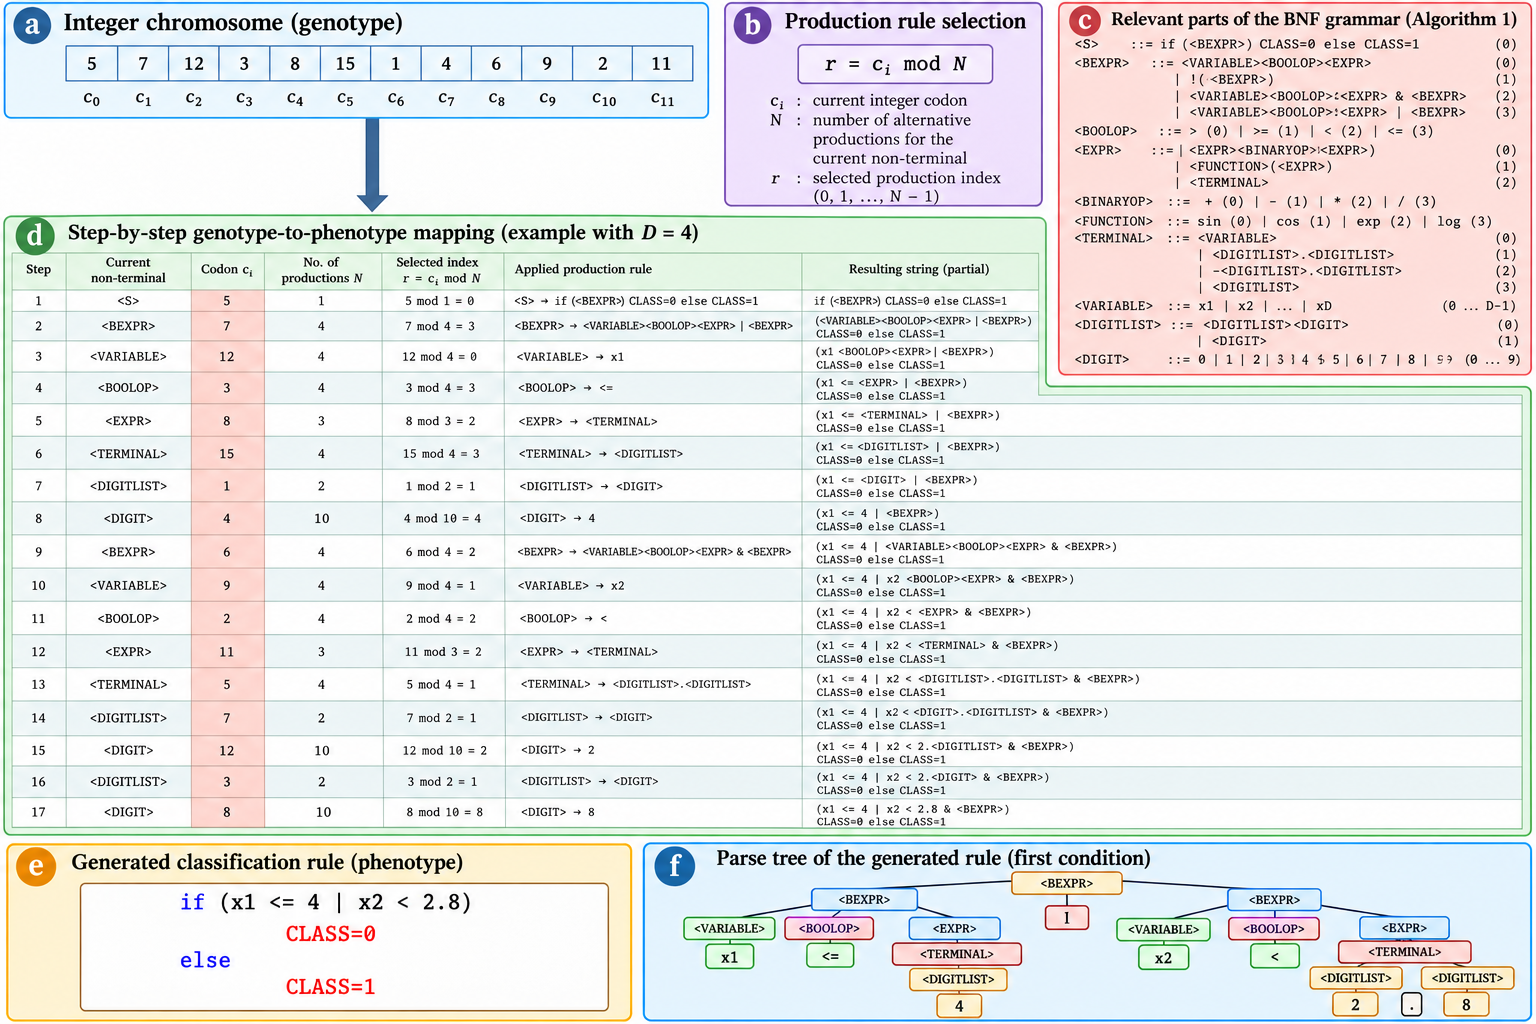
\includegraphics[scale=0.25]{mapping_new}
\par\end{centering}
\caption{Illustration of the genotype-to-phenotype mapping process employed
by GenClass. Integer-valued codons are sequentially mapped to BNF
production rules using the modulo operation until a complete classification
program is generated.\label{fig:genclass_mapping}}

\end{figure}

The main steps of the algorithm that produces classification programs
are listed subsequently.
\begin{enumerate}
\item \textbf{Initialization step}.
\begin{enumerate}
\item \textbf{Initialize} the Genetic Algorithm parameters: $N_{c}$, the
population size (number of chromosomes); $N_{g}$, the maximum number
of generations; $p_{s}$, the selection rate; and $p_{m}$, the mutation
rate.
\item \textbf{Generate }the initial population of $N_{c}$ chromosomes,
$g_{i},\;i=1,\ldots,N_{c}$, where each chromosome consists of a sequence
of randomly generated integer-valued codons.
\item \textbf{Set} $t=0$, the generation counter.
\end{enumerate}
\item \textbf{Fitness calculation step}.
\begin{enumerate}
\item \textbf{For} $i=1,\ldots,N_{c}$ \textbf{do}
\begin{enumerate}
\item \textbf{Map} each chromosome $g_{i}$ to its corresponding classification
program$C_{i}$ through the genotype-to-phenotype mapping process
defined by the BNF grammar presented in Algorithm \ref{alg:genclass_bnf}.
\item \textbf{Evaluate} the generated classification program $C_{i}$ on
the training set and compute its classification error. The resulting
error value, denoted by $f_{i}$, is used as the fitness value of
the corresponding chromosome $g_{i}$. 
\end{enumerate}
\item \textbf{End For}
\end{enumerate}
\item \textbf{Application of genetic operations}.
\begin{enumerate}
\item \textbf{Selection}: Rank the chromosomes according to their fitness
values in ascending order. The $(1-p_{s})N_{c}$ chromosomes with
the lowest fitness values are directly transferred to the next generation
without modification, while the remaining $p_{s}N_{c}$ chromosomes
are replaced by new offspring generated through the crossover and
mutation operators.
\item \textbf{Crossover}: Generate pairs of offspring by applying the one-point
crossover operator. For each pair of offspring, denoted as $O_{1}$
and $O_{2}$, two parent chromosomes, $P_{1}$ and $P_{2}$, are selected
from the current population using tournament selection. A crossover
point is then randomly selected along the chromosomes, and the genetic
material located after this point is exchanged between the two parents.
Consequently, $O_{1}$ inherits the first part of $P_{1}$ and the
second part of $P_{2}$, whereas $O_{2}$ inherits the first part
of $P_{2}$ and the second part of $P_{1}$. A graphical illustration
of the one-point crossover operation is provided in Figure \ref{fig:onePoint}.
\item \textbf{Mutation}: For each gene$g_{i,j}$ of chromosome $g_{i}$,
a random number $r\in[0,1]$ is generated. If $r\leq p_{m}$, where
$p_{m}$ denotes the mutation rate, the corresponding gene is replaced
by a randomly generated integer value within the predefined range
of admissible codon values. Otherwise, the gene remains unchanged.
\end{enumerate}
\item \textbf{Termination check step}.
\begin{enumerate}
\item \textbf{Set} $t=t+1$
\item \textbf{If} $t\le N_{g}$ \textbf{then go to} Fitness Calculation
step \textbf{else} terminate.
\end{enumerate}
\end{enumerate}
\begin{figure}[H]
\begin{centering}
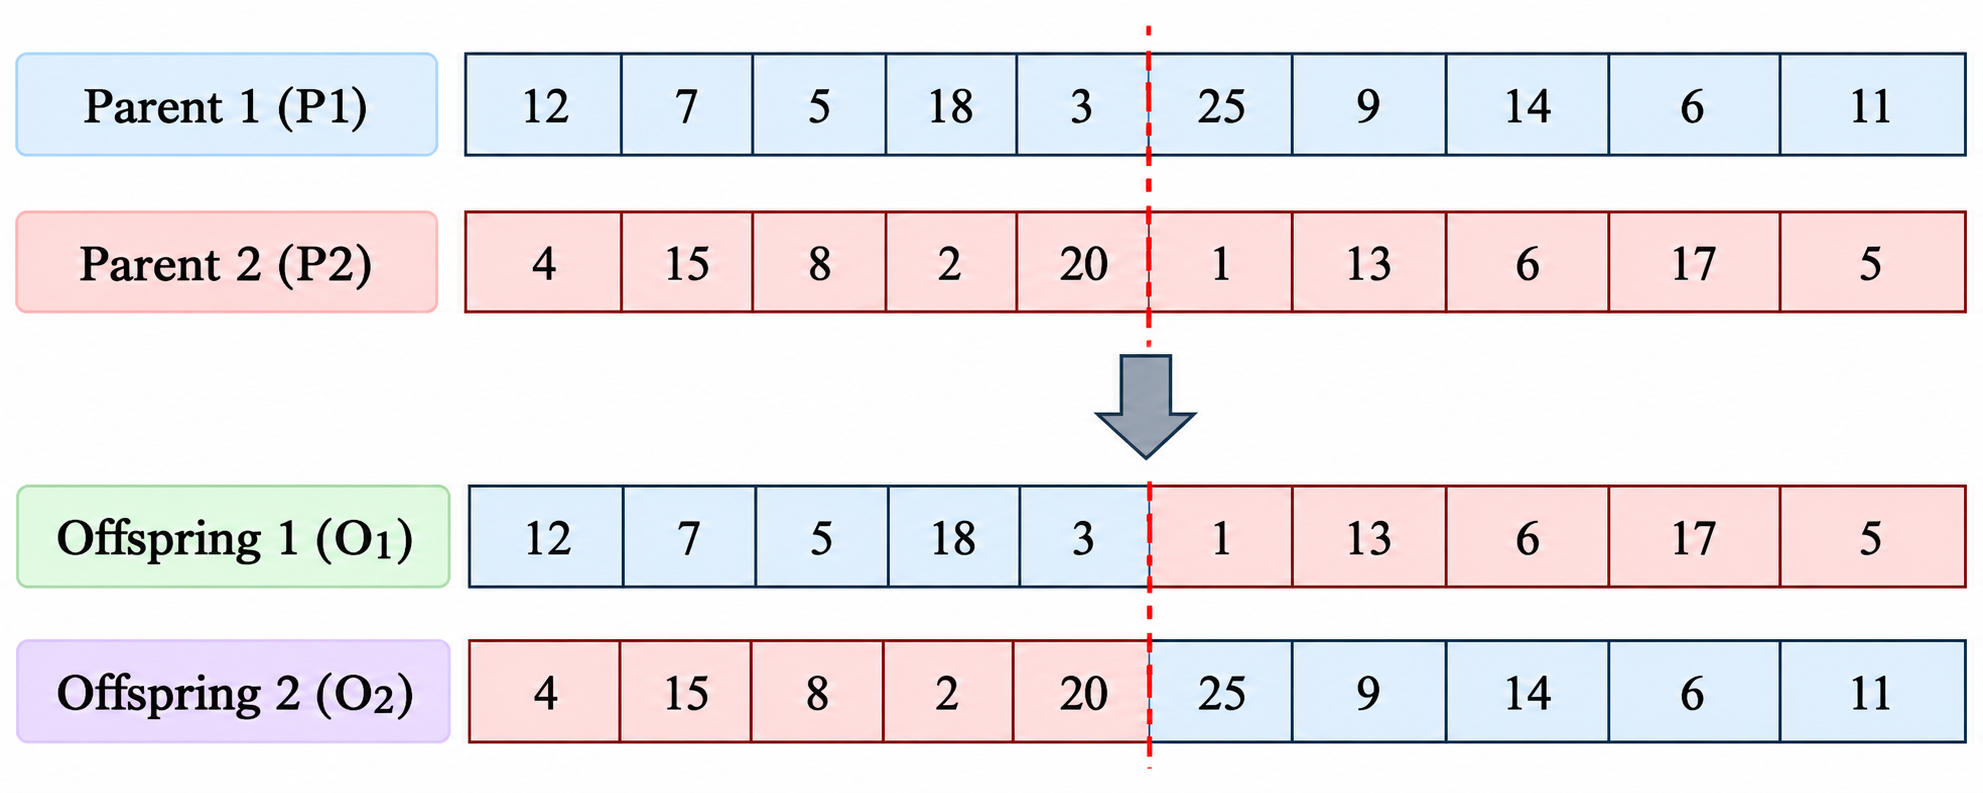
\includegraphics[scale=0.15]{onepoint}
\par\end{centering}
\caption{An example of the one - point crossover method.\label{fig:onePoint}}

\end{figure}


\subsection{The proposed crossover methods}

The additional crossover procedures investigated in this work can
be interpreted as crossover-based local improvement mechanisms embedded
within a conventional evolutionary algorithm. Their repeated application,
together with the immediate acceptance of fitness-improving modifications,
follows a greedy hill-climbing strategy in which candidate neighbors
are generated through recombination with other population members.
Consequently, the overall framework is closely related to hybrid evolutionary
and memetic algorithms, as discussed in subsection \ref{subsec:Hybrid-Evolutionary-and}.

In the present work, additional crossover techniques are introduced
with the aim of improving the performance of GenClass and enhancing
its ability to escape from local minima of the classification error
function. These crossover operations are applied at each generation
of the evolutionary process to a subset of the current population.
More specifically, a number of chromosomes are randomly selected from
the population and genetic material from each selected chromosome
is exchanged with that of another randomly selected chromosome. In
this way, new combinations of genetic material are introduced into
the population, potentially increasing population diversity and allowing
the evolutionary search to explore previously unvisited regions of
the search space. The number of chromosomes subjected to these additional
crossover operations at each generation is denoted by $\ensuremath{N_{K}}$
throughout the remainder of this work.

The proposed procedure is incorporated into the evolutionary algorithm
described in subsection \ref{subsec:The-rule-construction} and is
executed at each generation after the standard genetic operators of
selection, crossover, and mutation have been applied. In this way,
the additional crossover mechanism operates as an enhancement of the
original evolutionary process without modifying its basic structure.

The proposed crossover techniques, denoted throughout this work as
Standard, Targeted, and TargetedWorst, differ in the strategy employed
to select and exchange genetic material between chromosomes. A detailed
description of each technique is provided in the following subsections.

The Standard crossover strategy is closely related to the Local Crossover
operator previously introduced by Tsoulos et al. \citep{localCrossover}.
Both methods employ repeated one-point recombination with fitness-based
acceptance and sequential improvement of selected chromosomes. The
differences concern the selection of chromosomes for refinement, the
acceptance criterion, and the computational effort allocated to the
refinement stage. Therefore, Standard is considered here as an adapted
crossover-based refinement strategy rather than a fundamentally new
local-search operator. It also serves as a reference for evaluating
the additional grammatical and class-performance guidance introduced
by Targeted and TargetedWorst.

The configurations also differ substantially in the allocation of
search effort. The additional procedure performs $N_{K}k=200$ candidate
evaluations per generation, against $p_{s}N_{c}=450$ offspring produced
by the conventional operators. In the earlier study the corresponding
ratio is reversed by two orders of magnitude, since the refinement
stage dominates the evolutionary update. The additional crossover
examined here therefore operates as a supplementary refinement within
an otherwise conventional evolutionary search, rather than as its
principal search mechanism.

Targeted and TargetedWorst approaches introduce grammatical-category
matching, elite donor selection, bounded codon exchange and, for TargetedWorst,
class-performance-guided selection of the modified region. The use
of grammatical information to guide recombination is itself not new.
Harper and Blair \citep{ge_harper} introduced Matching Crossover,
which aligns corresponding grammatical positions, and LHS Replacement
Crossover, which exchanges complete expansions of matching non-terminals.
However, unlike complete-expansion replacement, the Targeted procedures
transfer bounded codon blocks beginning at grammatically matched positions
and therefore do not guarantee the preservation of complete grammatical
structures or of equivalent program behaviour after remapping.

\subsubsection{The Standard crossover method }

In the Standard crossover technique, for each of the $N_{K}$ selected
chromosomes, denoted by $g_{c}$, a subset of $k$ chromosomes is
randomly selected from the current population,

\[
S=\{g_{r_{1}},g_{r_{2}},\ldots,g_{r_{k}}\}.
\]

The chromosome $\ensuremath{g_{c}}$ is then successively combined
with each chromosome $\ensuremath{g_{r_{i}}},\ensuremath{i=1,\ldots,k}$,
using one-point crossover. For each pair $(g_{c},g_{r_{i}})$, a crossover
point is randomly selected and the corresponding genetic material
is exchanged to produce a candidate offspring chromosome $g_{\mathrm{new}}$.
The fitness of $g_{\mathrm{new}}$ is subsequently evaluated using
its classification error on the training set. If $g_{\mathrm{new}}$
achieves a lower fitness value than the current $g_{c}$, it replaces
$g_{c}$; otherwise, the current chromosome remains unchanged. Importantly,
whenever such an improvement occurs, the updated chromosome becomes
the new $g_{c}$ and is used in the subsequent crossover operation
with $g_{r_{i+1}}$. Therefore, the procedure performs a sequential
improvement of $g_{c}$, allowing beneficial genetic material obtained
from successive crossover operations to be accumulated. After all
$k$ chromosomes in $S$ have been examined, the final improved version
of $g_{c}$ is retained in the population.

The complete procedure of the Standard crossover technique is summarized
in Algorithm \ref{alg:standard_crossover}. The method follows a greedy
acceptance strategy, since a newly generated chromosome replaces the
current chromosome only when it achieves a lower classification error.
Furthermore, each accepted chromosome is immediately used in the subsequent
crossover operation, allowing improvements obtained during successive
crossover trials to be accumulated.

The proposed crossover operator generates up to two candidate offspring
using one-point crossover. The first offspring is constructed by combining
the prefix of the selected chromosome with the suffix of a randomly
selected chromosome. If this offspring improves the fitness of the
selected chromosome, it is accepted and replaces the original chromosome.
Otherwise, a second offspring is constructed by exchanging the corresponding
chromosome segments in the opposite direction. The second offspring
is accepted only if it improves the fitness of the selected chromosome.
If neither offspring yields an improvement, the original chromosome
remains unchanged. Thus, at most one offspring is accepted during
each crossover iteration.
\begin{center}
\begin{algorithm}[H]
\caption{Standard crossover technique}
\label{alg:standard_crossover}
\begin{algorithmic}[1]

\Require Population $G=\{g_1,g_2,\ldots,g_{N_c}\}$,
         number of selected chromosomes $N_K$,
         number of crossover trials $k$
\Ensure Updated population $G$

\State Randomly select $N_K$ chromosomes from $G$

\For{each selected chromosome $g_c$}

    \State Randomly select a subset
    $S=\{g_{r_1},g_{r_2},\ldots,g_{r_k}\}$ from $G$

    \For{$i=1$ to $k$}

        \State Randomly select a one-point crossover position

        \State Generate $g_{\mathrm{new}}$ by applying one-point crossover
        between $g_c$ and $g_{r_i}$

        \State Evaluate the fitness $f(g_{\mathrm{new}})$

        \If{$f(g_{\mathrm{new}}) < f(g_c)$}
            \State $g_c \gets g_{\mathrm{new}}$
        \EndIf

    \EndFor

\EndFor

\State \Return $G$

\end{algorithmic}
\end{algorithm}
\par\end{center}

\subsubsection{The Targeted crossover method }

In the Targeted crossover technique, the exchange of genetic material
is guided by information collected during the genotype-to-phenotype
mapping process. More specifically, the mapping procedure records
the positions of the active codons of each chromosome together with
their semantic role in the generated classification program. These
codons may correspond to different grammatical components, such as
functions, binary operators, Boolean operators, variables, and constants.

For each selected chromosome $g_{c}$, the Targeted technique performs
$k$ crossover trials. At each trial, an active codon position is
randomly selected as the target of the crossover operation. A donor
chromosome $g_{r}$ is then randomly selected from the best fraction
$\rho$ of the current population, and the recorded mapping information
is used to identify an active codon in $g_{r}$ having the same semantic
type as the selected codon of $g_{c}$. Instead of performing an unrestricted
one-point crossover, the Targeted technique transfers a bounded block
of genetic material between the corresponding positions. The size
of this block is determined from the distances to the next active
codons in the two chromosomes and is additionally restricted by a
predefined maximum block size $B_{\max}$. In this way, the transferred
genetic material is associated with similar grammatical components
of the classification programs represented by the two chromosomes.

An active codon is defined as a chromosome position actually accessed
during the genotype-to-phenotype mapping process. The proposed Targeted
crossover operator records these positions together with their associated
semantic categories, including functions, operators, variables, and
constants. A target codon is selected from this trace, and a compatible
donor codon of the same semantic category is selected from an elite
chromosome. The exchanged block length is determined by the distance
from each selected position to the next active codon with a greater
chromosome index, subject to the maximum block size and chromosome
boundaries. Consequently, when active codons occupy consecutive chromosome
positions, the exchanged block consists of a single codon. The operator
therefore performs semantically guided codon-level or short-block
exchanges rather than guaranteeing the exchange of complete grammatical
subtrees.

The resulting chromosome $g_{\mathrm{new}}$ is subsequently mapped
to its corresponding classification program and its fitness is evaluated
on the training set. If

\[
f\left(g_{\mathrm{new}}\right)<f\left(g_{c}\right),
\]

the new chromosome replaces $g_{c}$; otherwise, the current chromosome
remains unchanged. As in the Standard technique, an accepted improvement
is immediately retained and the updated chromosome is used in subsequent
crossover trials. The main difference from Standard crossover is therefore
that the exchange of genetic material is not determined exclusively
by randomly selected crossover points. Instead, information obtained
during the mapping process is exploited to perform crossover between
semantically related regions of the participating chromosomes. This
targeted exchange is intended to increase the probability of producing
meaningful modifications to the generated classification programs
while preserving useful genetic structures already discovered during
the evolutionary process. The complete procedure of the Targeted crossover
technique is summarized in Algorithm \ref{alg:targeted_crossover}.
\begin{center}
\begin{algorithm}[H]
\caption{Targeted crossover technique}
\label{alg:targeted_crossover}
\begin{algorithmic}[1]

\Require Population $G=\{g_1,g_2,\ldots,g_{N_c}\}$,
         number of selected chromosomes $N_K$,
         number of crossover trials $k$,
         elite fraction $\rho$,
         maximum block size $B_{\max}$
\Ensure Updated population $G$

\State Randomly select $N_K$ chromosomes from $G$
\State $N_e \gets \max(2,\lfloor \rho N_c \rfloor)$

\For{each selected chromosome $g_c$}

    \For{$i=1$ to $k$}

        \State Obtain the codon trace of the current chromosome $g_c$

        \State Construct the set $A_c$ of active semantic codons
        corresponding to functions, binary operators,
        Boolean operators, variables, and constants

        \If{$A_c$ is empty}
            \State \textbf{break}
        \EndIf

        \State Randomly select a target codon $a_c \in A_c$
        \State Let $t_c$ be the semantic type of $a_c$

        \State Randomly select a donor chromosome $g_r$
        from the best $N_e$ chromosomes, with $g_r \neq g_c$

        \State Obtain the codon trace of $g_r$

        \State Construct the set $A_r$ of active codons in $g_r$
        having semantic type $t_c$

        \If{$A_r$ is empty}
            \State \textbf{continue}
        \EndIf

        \State Randomly select a compatible donor codon $a_r \in A_r$

        \State Determine $L_c$, the distance from $a_c$
        to the next active codon in $g_c$

        \State Determine $L_r$, the distance from $a_r$
        to the next active codon in $g_r$

        \State $L \gets \min(L_c,L_r,B_{\max})$

        \State Create $g_{\mathrm{new}} \gets g_c$

        \State Copy $L$ codons from $g_r$, starting at $a_r$,
        to the corresponding block of $g_{\mathrm{new}}$
        starting at $a_c$

        \State Evaluate the fitness $f(g_{\mathrm{new}})$

        \If{$f(g_{\mathrm{new}}) < f(g_c)$}
            \State $g_c \gets g_{\mathrm{new}}$
        \EndIf

    \EndFor

\EndFor

\State \Return $G$

\end{algorithmic}
\end{algorithm}
\par\end{center}

\subsubsection{The TargetedWorst crossover method}

The TargetedWorst crossover technique extends the Targeted approach
by additionally exploiting information about the classification performance
of the generated program. While Targeted crossover may select an active
semantic codon from the chromosome without considering the performance
of individual classes, TargetedWorst attempts to concentrate the crossover
operation on the chromosome region associated with the class exhibiting
the poorest classification performance. The motivation behind this
strategy is to modify preferentially those parts of the generated
classification program that are more likely to contribute to the observed
classification errors, while leaving better-performing components
less affected.

The worst-performing class is identified using the class-specific
classification error computed on the training set. More specifically,
for each class c, the classification error is defined as the percentage
of incorrectly classified training patterns belonging to that class.
The class with the highest error rate is selected as the worst-performing
class. This criterion is equivalent to minimizing class-specific recall
and avoids directly favoring majority classes based on their absolute
number of misclassified patterns. Nevertheless, the estimated error
rates of classes containing relatively few training patterns may exhibit
higher variability, which represents a potential limitation of this
selection strategy.

For each selected chromosome $g_{c}$, the corresponding classification
program is evaluated and the class exhibiting the worst classification
performance is identified. The genotype-to-phenotype mapping information
is subsequently used to determine the active codons associated with
the corresponding part of the classification program. An active codon
is then selected from this region and its semantic type is determined.
As in the Targeted technique, a donor chromosome $g_{r}$ is selected
from the elite fraction of the population, and an active codon having
the same semantic type is identified in the donor chromosome. This
establishes semantically compatible positions between the two chromosomes
and allows genetic material from a high-quality solution to be transferred
specifically to a poorly performing region of $g_{c}$.

A bounded block of genetic material is subsequently transferred from
the donor chromosome to $g_{c}$. As in Targeted crossover, the size
of the transferred block is determined using the active-codon structure
of the participating chromosomes and is restricted by the predefined
maximum block size $B_{\max}$. The resulting chromosome $g_{\mathrm{new}}$
is then mapped to its corresponding classification program and evaluated
on the training set. If

\[
f\left(g_{\mathrm{new}}\right)<f\left(g_{c}\right),
\]

the candidate chromosome replaces $g_{c}$; otherwise, the modification
is discarded. Accepted improvements are immediately retained and are
therefore available to subsequent crossover trials.

Consequently, TargetedWorst introduces an additional level of guidance
compared with Targeted crossover. Targeted determines the exchanged
genetic material according to semantic information obtained during
genotype-to-phenotype mapping, whereas TargetedWorst combines this
information with class-specific classification performance in order
to focus the search on chromosome regions associated with poorly performing
parts of the generated classifier. The complete procedure is summarized
in Algorithm \ref{alg:targeted_worst_crossover}.
\begin{center}
\begin{algorithm}[H]
\caption{TargetedWorst crossover technique}
\label{alg:targeted_worst_crossover}
\begin{algorithmic}[1]

\Require Population $G=\{g_1,g_2,\ldots,g_{N_c}\}$,
         number of selected chromosomes $N_K$,
         number of crossover trials $k$,
         elite fraction $\rho$,
         maximum block size $B_{\max}$
\Ensure Updated population $G$

\State Randomly select $N_K$ chromosomes from $G$
\State $N_e \gets \max(2,\lfloor \rho N_c \rfloor)$

\For{each selected chromosome $g_c$}

    \For{$i=1$ to $k$}

        \State Evaluate the class-specific performance of $g_c$
        \State Identify the worst-performing class $w$

        \State Let $C$ be the number of classes
        \State $N_R \gets C-1$

        \If{$w < N_R$}
            \State Determine the chromosome segment $R_w$
                   associated with class $w$
        \Else
            \State Set $R_w$ to the entire chromosome
        \EndIf

        \State Obtain the codon trace of the current chromosome $g_c$

        \State Construct the set $A_c$ of active semantic codons
               of $g_c$ that belong to $R_w$

        \If{$A_c$ is empty}
            \State \textbf{continue}
        \EndIf

        \State Randomly select a target codon $a_c \in A_c$
        \State Let $t_c$ be the semantic type of $a_c$

        \State Randomly select a donor chromosome $g_r$
               from the best $N_e$ chromosomes,
               with $g_r \neq g_c$

        \State Obtain the codon trace of $g_r$

        \If{$w < N_R$}
            \State Determine the donor segment $R_w^{(r)}$
                   associated with class $w$
        \Else
            \State Set $R_w^{(r)}$ to the entire donor chromosome
        \EndIf

        \State Construct the set $A_r$ of active codons in $g_r$
               that belong to $R_w^{(r)}$ and have semantic type $t_c$

        \If{$A_r$ is empty}
            \State \textbf{continue}
        \EndIf

        \State Randomly select a compatible donor codon $a_r \in A_r$

        \State Determine $L_c$, the distance from $a_c$
               to the next active codon in $g_c$

        \State Determine $L_r$, the distance from $a_r$
               to the next active codon in $g_r$

        \State $L \gets \min(L_c,L_r,B_{\max})$

        \State Restrict $L$ to remain within the corresponding
               class segments and chromosome boundaries

        \State Create $g_{\mathrm{new}} \gets g_c$

        \State Copy $L$ codons from $g_r$, starting at $a_r$,
               to $g_{\mathrm{new}}$, starting at $a_c$

        \State Evaluate the fitness $f(g_{\mathrm{new}})$

        \If{$f(g_{\mathrm{new}}) < f(g_c)$}
            \State $g_c \gets g_{\mathrm{new}}$
        \EndIf

    \EndFor

\EndFor

\State \Return $G$

\end{algorithmic}
\end{algorithm}
\par\end{center}

Figure \ref{fig:Flowchart-of-the} presents the general flowchart
of the proposed method. The process starts with the generation of
the initial population of integer-valued chromosomes. Each chromosome
is mapped to a classification program through the BNF grammar, and
the program is evaluated on the training set, which gives the fitness
of the chromosome. The standard genetic operators of selection, one-point
crossover and mutation are then applied to the population. After them,
the additional crossover procedure is executed. A small number of
chromosomes is randomly selected and, for each of them, a number of
crossover trials is performed. In every trial, the technique in use,
Standard, Targeted or TargetedWorst, produces a new candidate chromosome,
which is mapped to a classification program through the grammar and
evaluated. If the candidate achieves a lower error than the current
chromosome, it replaces it, otherwise the current chromosome is kept.
The process continues with the next trial until all the trials of
all the selected chromosomes are completed. Finally, the termination
criterion is checked. If it is not satisfied, the algorithm returns
to the mapping and evaluation of the new population, otherwise it
terminates and returns the best classification program.

\begin{figure}[H]
\begin{centering}
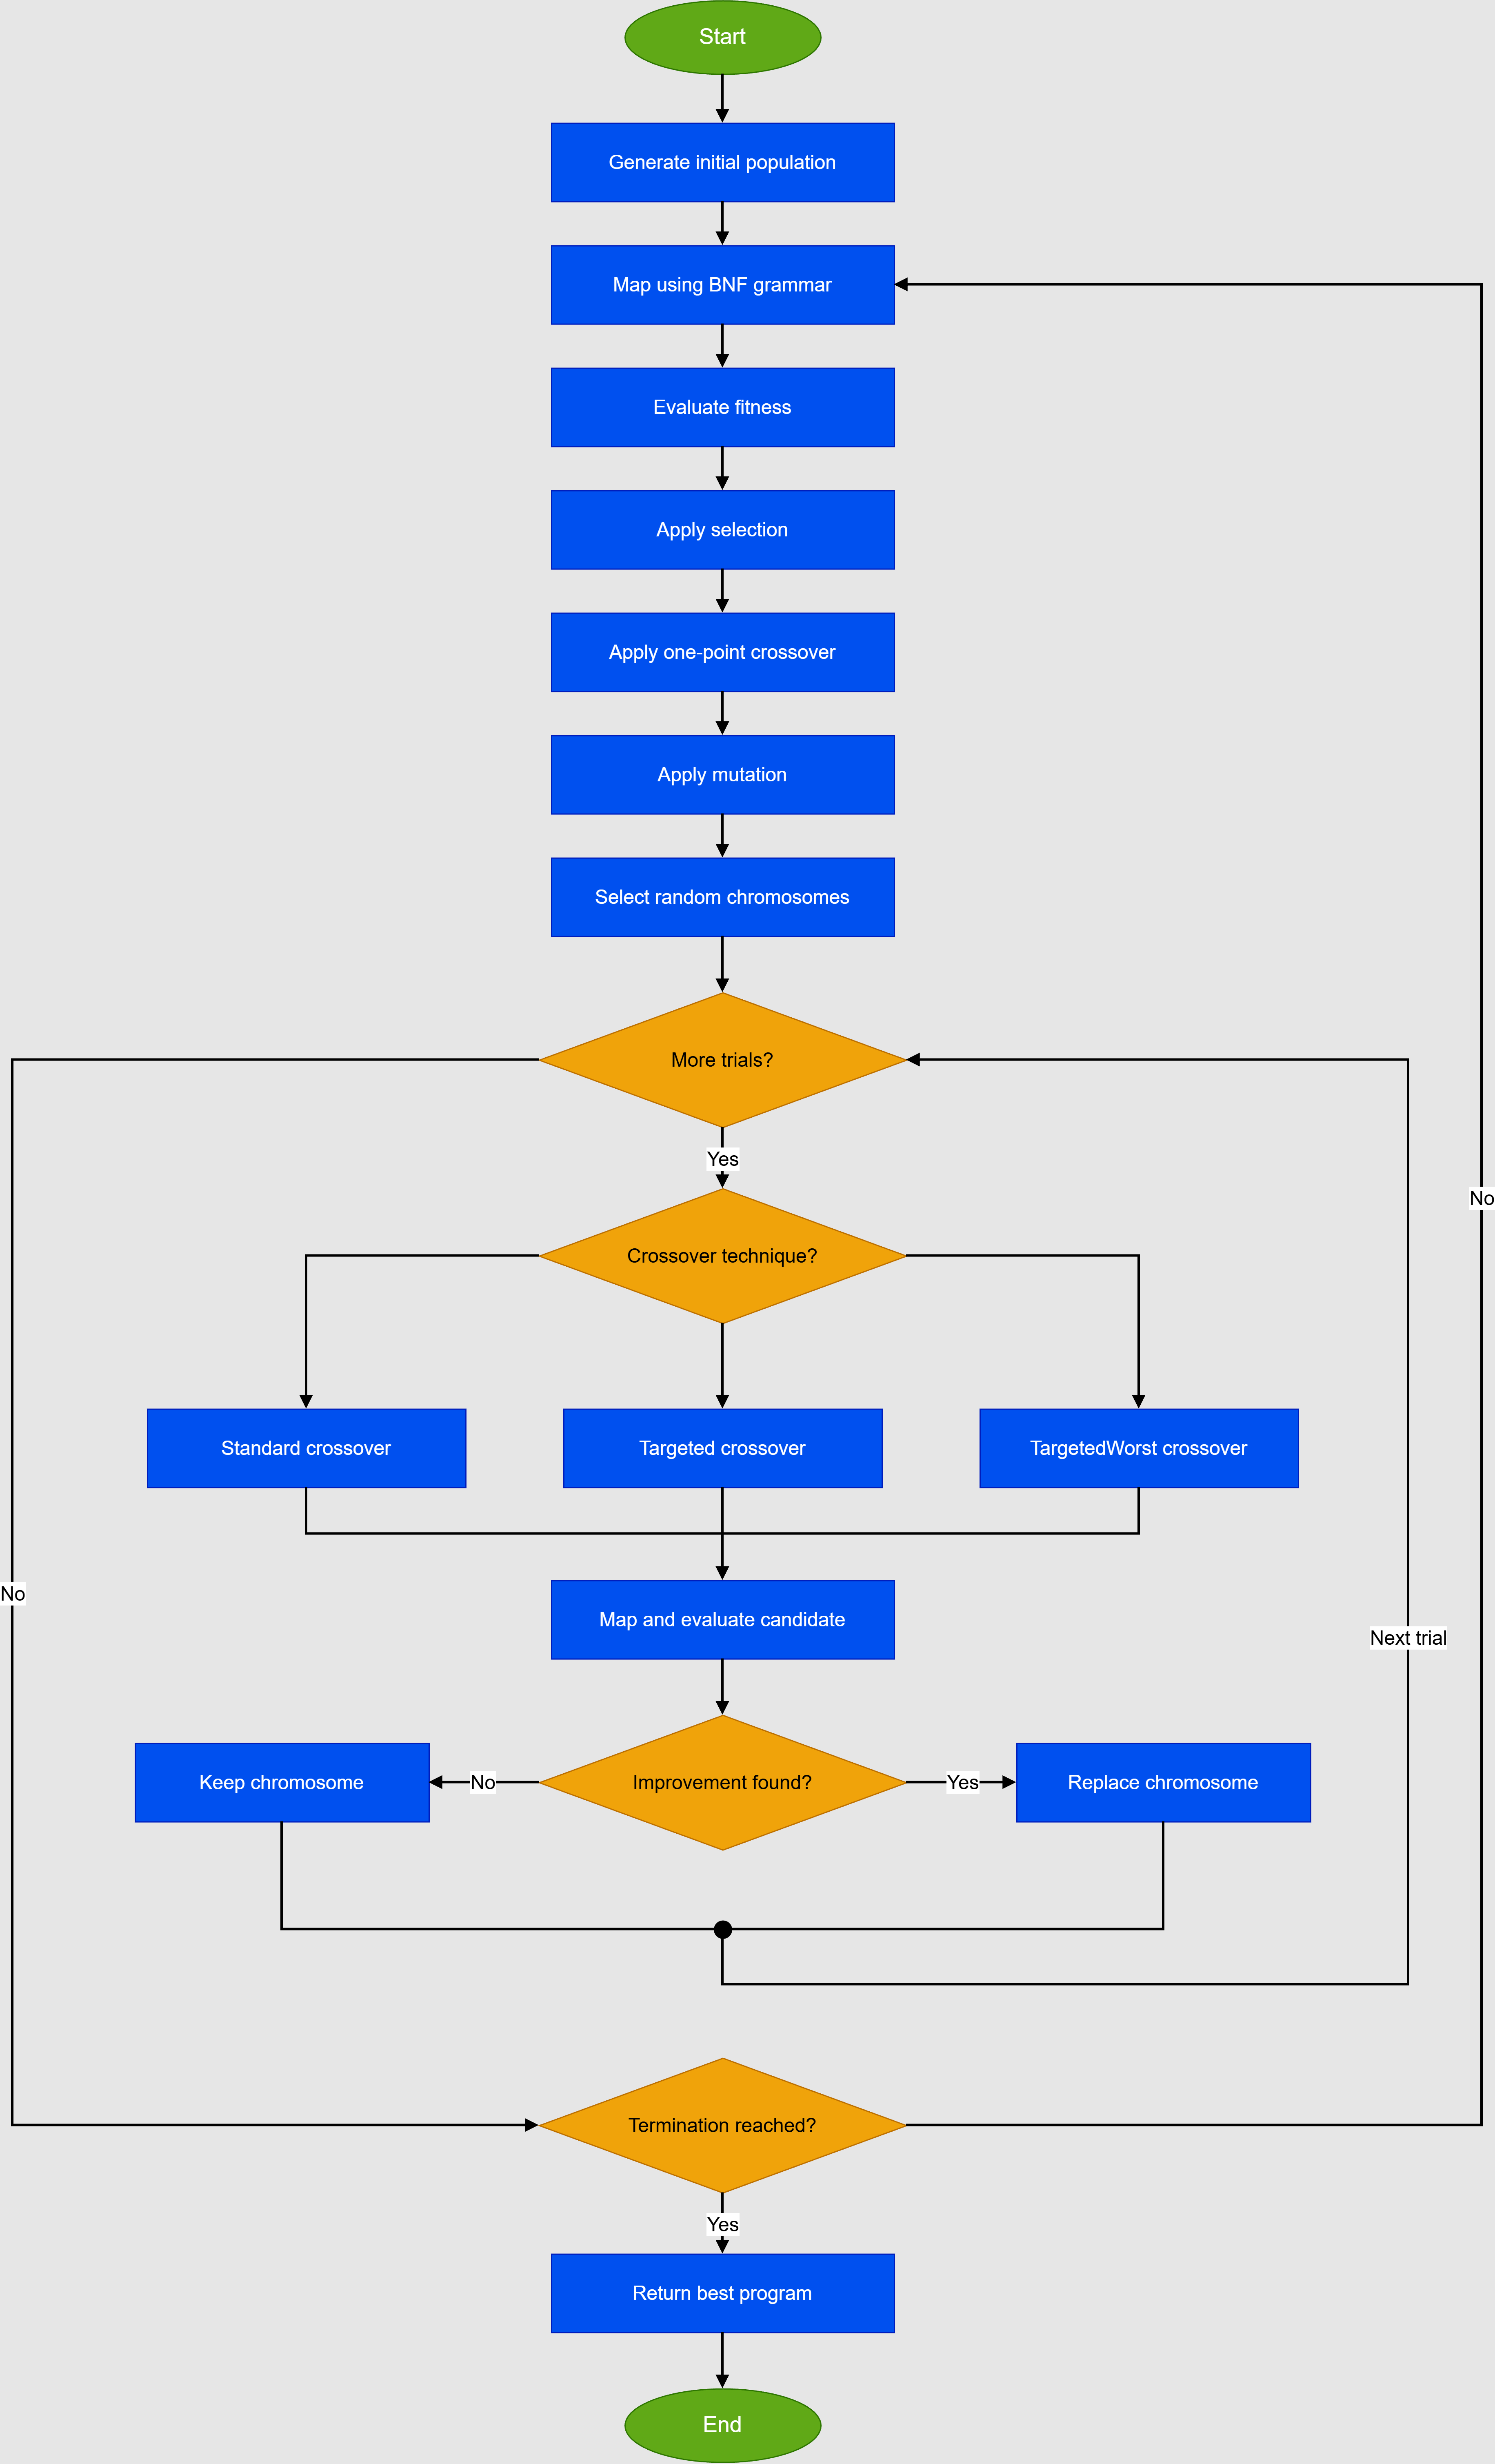
\includegraphics[scale=0.3]{flowchart}
\par\end{centering}
\caption{Flowchart of the proposed GenClass method with the additional crossover
techniques.\label{fig:Flowchart-of-the}}

\end{figure}


\section{Results\label{sec:Results}}

\subsection{Experimental datasets }

The datasets employed in the experimental evaluation were obtained
from two widely used public repositories: the UCI Machine Learning
Repository \citep{uci} and the KEEL Dataset Repository \citep{Keel}.
Both repositories provide a broad collection of benchmark datasets
commonly used for the experimental evaluation and comparison of machine
learning and classification algorithms. The datasets were accessed
on 3 October 2026. The used datasets are the following:
\begin{enumerate}
\item \textbf{Alcohol. }This dataset contains data collected from experiments
investigating patterns of alcohol consumption and is used as a classification
benchmark in the present study \citep{alcohol}. 
\item \textbf{Appendicitis.} The Appendicitis dataset is a binary classification
dataset containing 106 instances and 7 numerical features, used to
predict the presence or absence of acute appendicitis based on clinical
measurements \citep{appendicitis}. 
\item The \textbf{Beed} dataset. The Bangalore EEG Epilepsy Dataset (BEED),
presented by Banu et al. \citep{beed}, is an EEG dataset developed
for epileptic seizure detection and classification. The dataset contains
8,000 patterns, each represented by 16 features.
\item \textbf{Dermatology. }The Dermatology dataset \citep{dermatology}
contains clinical and histopathological measurements used for the
differential diagnosis of dermatological diseases.
\item \textbf{Gene}. The Gene dataset, also known as the Splice-junction
Gene Sequences dataset, contains 3,175 DNA sequences represented by
120 binary features. The dataset is used for the classification of
splice-junction boundaries into three classes: exon--intron (EI)
boundaries, intron--exon (IE) boundaries, and sequences containing
neither type of boundary \citep{gene}.
\item \textbf{Hayes-Roth. }The Hayes-Roth dataset is an artificial classification
dataset comprising three classes and was originally designed to evaluate
the behavior of prototype-based classifiers. The hobby attribute was
generated randomly and therefore acts as a noise-inducing feature
in the classification problem \citep{hayes-roth}.
\item \textbf{Hepatitis. }The Hepatitis dataset contains clinical information
collected from patients affected by hepatitis and includes a combination
of integer- and real-valued attributes describing various patient
characteristics and medical measurements \citep{hepatitis}.
\item \textbf{HouseVotes.} The House Votes dataset contains voting records
of members of the U.S. House of Representatives on a set of congressional
issues. The classification task aims to distinguish representatives
according to their political party affiliation based on their recorded
votes \citep{housevotes}.
\item \textbf{Ionosphere. }The Ionosphere dataset contains radar measurements
collected from signals transmitted through the ionosphere. The classification
task aims to distinguish between radar returns that provide evidence
of structure in the ionosphere and those that do not \citep{ion1,ion2}.
\item \textbf{Lymphography} \citep{lymography}, which is a dataset with
four distinct classes.
\item \textbf{Nursery. }The Nursery dataset was derived from a hierarchical
decision model originally developed to rank applications for admission
to nursery schools. The model was used in Ljubljana, Slovenia, during
the 1980s, when high demand for nursery schools required an objective
procedure for evaluating and explaining admission decisions. The corresponding
classification task involves assigning nursery school applications
to different priority categories based on a set of socioeconomic and
family-related attributes \citep{nursery}.
\item \textbf{Optdigits}. The Optical Recognition of Handwritten Digits
(Optdigits) dataset contains digitized representations of handwritten
numerals obtained from optical scans. The corresponding classification
task aims to recognize and assign each handwritten sample to one of
the ten digit classes, ranging from 0 to 9 \citep{optdigits}.
\item \textbf{Penbased}. The Pen-Based Recognition of Handwritten Digits
dataset contains samples of handwritten digits collected from 44 writers.
Each digit is represented using its $(x,y)$ coordinate information,
resampled to eight points and encoded as a fixed-length feature vector
of 16 attributes. The corresponding classification task aims to assign
each sample to one of the ten digit classes, ranging from 0 to 9 \citep{penbased}.
\item \textbf{Phoneme}. The Phoneme dataset contains acoustic measurements
extracted from speech signals. The corresponding classification task
aims to distinguish between nasal and oral phonemes based on their
acoustic characteristics \citep{phoneme}.
\item \textbf{PirVision. }The PirVision dataset contains sensor measurements
collected for occupancy detection. The corresponding classification
task aims to determine occupancy status based on data acquired from
passive infrared (PIR) sensing devices \citep{pirvision}.
\item \textbf{Satimage}. The Satimage dataset contains multispectral satellite
image data representing different types of terrain. The corresponding
classification task aims to assign image regions to different land-cover
classes based on their spectral characteristics \citep{satimage}.
\item \textbf{Segment. }The Segment dataset contains image regions characterized
by a set of numerical features extracted from outdoor images. The
corresponding classification task aims to assign each region to one
of several image categories based on its visual characteristics \citep{segment}.
\item \textbf{Shuttle. }The Shuttle dataset was originally developed to
derive comprehensible classification rules for determining the conditions
under which automatic landing control of a spacecraft would be preferable
to manual control. The corresponding classification task involves
distinguishing among different operational conditions based on a set
of numerical measurements \citep{shuttle}.
\item \textbf{Spambase}. The Spambase dataset contains features extracted
from email messages, including word and character frequencies as well
as information related to sequences of capital letters. The corresponding
binary classification task aims to distinguish spam from non-spam
emails \citep{spambase}.
\item \textbf{Spiral}, The Spiral dataset is a synthetic binary classification
problem consisting of 1,000 two-dimensional instances equally distributed
between two classes. The instances are generated using parametric
equations that form two intertwined spiral patterns, resulting in
a highly nonlinear classification problem \citep{spiral}. 
\item \textbf{Student. }The Student dataset contains educational data collected
from 587 students over two consecutive academic years in ten non-university
educational centers. The attributes describe factors such as academic
performance, student abilities, motivation, and methodological and
assessment preferences. The corresponding classification task aims
to categorize students according to their educational characteristics
and performance \citep{student}.
\item \textbf{Splice} dataset, which is a biological classification benchmark
consisting of 3,190 DNA sequences, each represented by 60 categorical
features. The task is to classify sequences into three categories:
exon-intron boundaries (EI), intron-exon boundaries (IE), and non-splice
junctions (N) \citep{splice} .
\item \textbf{Texture.} The Texture dataset is designed for the classification
of different visual textures and comprises 11 texture classes, including
grass lawn, pressed calf leather, handmade paper, raffia, and cotton
canvas. Each pattern corresponds to a pixel represented by 40 numerical
features obtained from the estimation of fourth-order modified moments
computed at four different orientations$:\ensuremath{0^{\circ}},\ensuremath{45^{\circ}},\ensuremath{90^{\circ}},$
and $135^{\circ}$. The corresponding classification task aims to
assign each pattern to one of the 11 texture categories \citep{texture}.
\item \textbf{Thyroid. }The Thyroid dataset contains clinical measurements
related to thyroid gland function. The corresponding classification
task aims to determine whether a patient exhibits normal thyroid function
or suffers from hyperthyroidism or hypothyroidism, resulting in a
three-class classification problem \citep{thyroid}.
\item The \textbf{TwoNorm} dataset is a synthetic 20-dimensional binary
classification problem originally introduced by Breiman. The patterns
of each class are generated from multivariate normal distributions
with unit covariance matrices and symmetric mean vectors. Specifically,
the two class means are $(a,a,\ldots,a)$ and $(-a,-a,\ldots,-a)$,
where $a=2/\sqrt{20}$ \citep{twonorm}.
\item \textbf{Vehicle. }The Vehicle dataset is designed to classify vehicle
silhouettes into four different categories using a set of numerical
features extracted from their shapes. The silhouettes were obtained
from vehicles viewed from different angles, making the classification
task dependent on distinguishing characteristic geometric properties
despite variations in viewing orientation \citep{vehicle}.
\item \textbf{Yeast. }The Yeast dataset contains information describing
proteins from Saccharomyces cerevisiae. Each protein is represented
by eight numerical features derived from sequence-based measurements.
The corresponding classification task aims to predict the cellular
localization site of each protein among ten possible classes \citep{yeast}.
\item \textbf{EEG}. The EEG dataset is a medical dataset containing electroencephalographic
recordings obtained from healthy subjects and patients with epilepsy
under different physiological and pathological conditions \citep{eeg1,eeg2}.
The original dataset consists of five subsets, denoted by Z, O, N,
F, and S, corresponding to different recording conditions and brain
states. From these subsets, four classification problems were constructed
for the experimental evaluation: Z\_F\_S, ZO\_NF\_S, Z\_O\_N\_F\_S,
and ZONF\_S.
\end{enumerate}
\begin{table}[H]
\caption{The main characteristics of each dataset.\label{tab:The-main-characteristics}}

\centering{}%
\begin{tabular}{|c|c|c|c|}
\hline 
DATASET & FEATURES & PATTERNS & CLASSES\tabularnewline
\hline 
\hline 
ALCOHOL & 154 & 476 & 4\tabularnewline
\hline 
APPENDICITIS & 7 & 106 & 2\tabularnewline
\hline 
BEED & 16 & 8000 & 4\tabularnewline
\hline 
DERMATOLOGY & 34 & 358 & 6\tabularnewline
\hline 
GENE & 120 & 3175 & 3\tabularnewline
\hline 
HAYES ROTH & 5 & 160 & 3\tabularnewline
\hline 
HEPATITIS & 19 & 80 & 2\tabularnewline
\hline 
HOUSEVOTES & 16 & 232 & 2\tabularnewline
\hline 
IONOSPHERE & 34 & 351 & 2\tabularnewline
\hline 
LYMPHOGRAPHY & 18 & 148 & 4\tabularnewline
\hline 
NURSERY & 8 & 12960 & 5\tabularnewline
\hline 
OPTDIGITS & 64 & 5620 & 10\tabularnewline
\hline 
PENBASED & 16 & 10992 & 10\tabularnewline
\hline 
PHONEME & 5 & 5404 & 2\tabularnewline
\hline 
PIRVISION & 56 & 15302 & 3\tabularnewline
\hline 
SATIMAGE & 36 & 6435 & 7\tabularnewline
\hline 
SEGMENT & 19 & 2310 & 7\tabularnewline
\hline 
SHUTTLE & 9 & 58000 & 7\tabularnewline
\hline 
SPAMBASE & 57 & 4597 & 2\tabularnewline
\hline 
SPIRAL & 2 & 2000 & 2\tabularnewline
\hline 
SPLICE & 60 & 3190 & 3\tabularnewline
\hline 
STUDENT & 5 & 587 & 4\tabularnewline
\hline 
TEXTURE & 40 & 5500 & 11\tabularnewline
\hline 
THYROID & 21 & 7200 & 3\tabularnewline
\hline 
TWONORM & 20 & 7400 & 2\tabularnewline
\hline 
VEHICLE & 18 & 846 & 4\tabularnewline
\hline 
YEAST & 8 & 1484 & 10\tabularnewline
\hline 
Z\_F\_S & 21 & 300 & 3\tabularnewline
\hline 
Z\_O\_N\_F\_S & 21 & 500 & 5\tabularnewline
\hline 
ZO\_NF\_S & 21 & 500 & 3\tabularnewline
\hline 
ZONF\_S & 21 & 500 & 2\tabularnewline
\hline 
\end{tabular}
\end{table}


\subsection{Experimental results }

The proposed method was implemented in C++. For each dataset, a 10-fold
cross-validation procedure was employed using predefined training
and test partitions. Each experiment was repeated 30 times independently
for every fold, resulting in a total of 300 runs per dataset and method.
In each run, the classification model was constructed and optimized
exclusively using the training partition, while its classification
error was evaluated on the corresponding held-out test partition.
The final classification error reported in the experimental tables
was calculated as the arithmetic mean of the 300 test classification
errors. The test partitions were not used during the evolutionary
optimization process. The code used in the experiments with GenClass
is a modifed version of the original algorithm located in the repository
\url{https://github.com/itsoulos/QGenClass/}(accessed on 24 October
2026). The values used for the experimental parameters are listed
in Table \ref{tab:Values-for-the}. 

\begin{table}[H]
\caption{Values for the parameters in experiments.\label{tab:Values-for-the}}

\begin{centering}
\begin{tabular}{|c|c|c|}
\hline 
PARAMETER & MEANING & VALUE\tabularnewline
\hline 
\hline 
$N_{c}$ & Number of chromosomes & 500\tabularnewline
\hline 
$N_{g}$ & Number of allowed generations & 500\tabularnewline
\hline 
$N_{s}$ & Chromosome length & 200\tabularnewline
\hline 
$N_{t}$ & Tournament size & 20\tabularnewline
\hline 
$w$ & Maximum wrapping & 2\tabularnewline
\hline 
$p_{s}$ & Selection rate & 0.9\tabularnewline
\hline 
$p_{m}$ & Mutation rate & 0.05\tabularnewline
\hline 
$N_{K}$ & Crossover items & 10\tabularnewline
\hline 
$k$ & Number of crossover trials & 20\tabularnewline
\hline 
$\rho$ & Elite fraction for donor selection & 0.20\tabularnewline
\hline 
$B_{\mbox{max}}$ & Maximum crossover block size & 16\tabularnewline
\hline 
\end{tabular}
\par\end{centering}
\end{table}
 The notation used in Table \ref{tab:methods_comparison} is described
below:
\begin{enumerate}
\item DATASET denotes the dataset used in the corresponding experiment.
\item RBFCON, this method was presented recently \citep{rbfcon} to construct
Radial Basis Function (RBF) neural networks, with the assistance of
Grammatical Evolution. The parameters used for this method are presented
in Table \ref{tab:Values-for-the}.
\item CART, denotes the Classification and Regression Trees (CART) algorithm
\citep{cart} used to construct binary decision trees by recursively
partitioning the feature space. For classification tasks, the splits
are typically selected using the Gini impurity criterion, while tree
pruning can be employed to reduce overfitting .
\item SVM, Support Vector Machines (SVMs) \citep{svm} was also used here
and was implemented using the LIBSVM library \citep{libsvm}.
\item RBF denotes a Radial Basis Function (RBF) neural network \citep{rbf1,rbf2}
with $H=10$ hidden nodes.
\item NEAT denotes the NeuroEvolution of Augmenting Topologies (NEAT) method
\citep{neat}.
\item DNN denotes a deep neural network implemented using the Tiny-DNN library,
publicly available at the project's GitHub repository \url{https://github.com/tiny-dnn/tiny-dnn}(accessed
on 27 October 2026). The network was trained using the AdaGrad optimization
algorithm \citep{adagrad}.
\item ADAM denotes a neural network with $H=10$ hidden nodes trained using
the Adam optimization algorithm \citep{nn_adam}.
\item BFGS denotes a neural network with $H=10$ hidden nodes trained using
Powell's variant of the BFGS optimization method \citep{powell}.
\item GEN denotes a neural network with $H=10$ hidden nodes whose weights
were optimized using a Genetic Algorithm. The Genetic Algorithm employed
the same parameter settings reported in Table \ref{tab:Values-for-the}.
\item CLASS denotes the original GenClass rule construction method without
the additional crossover mechanism proposed in this work. The parameters
used for this method are presented in Table \ref{tab:Values-for-the}.
\item STANDARD denotes GenClass enhanced with the proposed Standard crossover
method. The parameters used for this method are presented in Table
\ref{tab:Values-for-the}.
\item The row AVERAGE reports the mean classification error across all datasets
for the corresponding method.
\end{enumerate}
\begin{landscape}
\begin{center}
{\tiny{}%
\begin{longtable}[c]{|c|c|c|c|c|c|c|c|c|c|c|c|}
\caption{Classification error (\%) of the proposed method (STANDARD) and of
the other classifiers on the 31 datasets. STANDARD is the GenClass
method with the proposed additional crossover procedure, while CLASS
is the original GenClass method without it. The last row (AVERAGE)
reports the mean error over all datasets, and lower values indicate
better performance.\label{tab:methods_comparison}}
\tabularnewline
\endfirsthead
\caption{Classification error (\%) of the proposed method (STANDARD) and of
the other classifiers on the 31 datasets. STANDARD is the GenClass
method with the proposed additional crossover procedure, while CLASS
is the original GenClass method without it. The last row (AVERAGE)
reports the mean error over all datasets, and lower values indicate
better performance.\label{tab:methods_comparison}}
\tabularnewline
\endhead
\hline 
DATASET & RBFCON & CART & SVM & RBF & NEAT & DNN & ADAM & BFGS & GEN & CLASS & STANDARD\tabularnewline
\hline 
\hline 
ALCOHOL & 20.43\% & 23.83\% & 23.40\% & 49.38\% & 66.80\% & 39.04\% & 57.78\% & 41.50\% & 39.57\% & 16.70\% & 11.70\%\tabularnewline
\hline 
APPENDICITIS & 17.80\% & 16.00\% & 21.00\% & 12.23\% & 17.20\% & 17.30\% & 16.50\% & 18.00\% & 18.10\% & 16.47\% & 12.80\%\tabularnewline
\hline 
BEED & 43.01\% & 38.17\% & 32.17\% & 65.12\% & 67.94\% & 64.45\% & 70.38\% & 75.24\% & 46.19\% & 31.93\% & 27.45\%\tabularnewline
\hline 
DERMATOLOGY & 39.80\% & 7.14\% & 11.14\% & 59.48\% & 32.43\% & 24.26\% & 26.14\% & 52.92\% & 30.58\% & 5.69\% & 2.80\%\tabularnewline
\hline 
GENE & 50.86\% & 30.19\% & 9.21\% & 37.11\% & 52.68\% & 33.06\% & 35.17\% & 38.12\% & 34.38\% & 8.67\% & 7.29\%\tabularnewline
\hline 
HAYES ROTH & 40.08\% & 37.59\% & 55.39\% & 64.36\% & 50.15\% & 44.65\% & 59.70\% & 37.33\% & 56.18\% & 24.31\% & 21.08\%\tabularnewline
\hline 
HEPATITIS & 13.13\% & 21.25\% & 16.25\% & 18.38\% & 39.75\% & 16.65\% & 16.25\% & 21.38\% & 15.00\% & 15.50\% & 12.00\%\tabularnewline
\hline 
HOUSEVOTES & 4.61\% & 4.33\% & 7.32\% & 6.13\% & 10.89\% & 3.13\% & 7.48\% & 7.13\% & 6.62\% & 3.47\% & 2.96\%\tabularnewline
\hline 
IONOSPHERE & 12.83\% & 9.14\% & 6.12\% & 16.22\% & 19.67\% & 12.57\% & 16.64\% & 15.29\% & 15.14\% & 8.10\% & 8.74\%\tabularnewline
\hline 
LYMPHOGRAPHY & 24.57\% & 22.86\% & 22.71\% & 25.50\% & 33.70\% & 24.07\% & 39.79\% & 35.43\% & 28.42\% & 22.67\% & 18.86\%\tabularnewline
\hline 
NURSERY & 44.24\% & 17.94\% & 24.62\% & 77.10\% & 64.11\% & 59.73\% & 40.94\% & 41.40\% & 32.14\% & 19.65\% & 22.27\%\tabularnewline
\hline 
OPTDIGITS & 62.29\% & 32.94\% & 26.62\% & 71.97\% & 72.56\% & 64.34\% & 72.32\% & 67.13\% & 67.81\% & 27.15\% & 14.77\%\tabularnewline
\hline 
PENBASED & 60.33\% & 18.00\% & 26.81\% & 81.69\% & 78.58\% & 73.50\% & 77.41\% & 82.48\% & 84.01\% & 24.93\% & 17.79\%\tabularnewline
\hline 
PHONEME & 15.59\% & 18.60\% & 21.56\% & 23.32\% & 22.43\% & 24.34\% & 29.43\% & 15.58\% & 15.55\% & 18.89\% & 16.82\%\tabularnewline
\hline 
PIRVISION & 8.14\% & 1.15\% & 2.05\% & 24.58\% & 11.84\% & 18.28\% & 18.38\% & 16.94\% & 14.31\% & 6.53\% & 4.38\%\tabularnewline
\hline 
SATIMAGE & 32.97\% & 23.12\% & 10.86\% & 40.19\% & 76.19\% & 72.30\% & 73.22\% & 71.73\% & 54.54\% & 18.47\% & 16.14\%\tabularnewline
\hline 
SEGMENT & 32.47\% & 17.45\% & 30.46\% & 59.68\% & 66.72\% & 32.04\% & 49.75\% & 68.97\% & 57.72\% & 15.21\% & 9.57\%\tabularnewline
\hline 
SHUTTLE & 23.25\% & 0.36\% & 0.32\% & 32.83\% & 29.32\% & 2.27\% & 21.29\% & 42.07\% & 20.86\% & 1.11\% & 1.28\%\tabularnewline
\hline 
SPAMBASE & 10.54\% & 13.18\% & 9.33\% & 29.35\% & 35.77\% & 11.30\% & 48.05\% & 18.16\% & 6.37\% & 8.97\% & 7.28\%\tabularnewline
\hline 
SPIRAL & 41.03\% & 41.70\% & 54.30\% & 44.87\% & 48.66\% & 45.24\% & 47.67\% & 47.99\% & 48.66\% & 35.65\% & 31.25\%\tabularnewline
\hline 
SPLICE & 28.37\% & 15.83\% & 14.61\% & 40.27\% & 55.54\% & 48.18\% & 75.93\% & 30.64\% & 30.97\% & 7.68\% & 7.62\%\tabularnewline
\hline 
STUDENT & 12.43\% & 7.93\% & 4.70\% & 5.49\% & 10.20\% & 6.93\% & 5.13\% & 7.14\% & 5.61\% & 6.86\% & 5.72\%\tabularnewline
\hline 
TEXTURE & 46.87\% & 35.44\% & 24.55\% & 74.52\% & 70.82\% & 70.78\% & 56.33\% & 59.25\% & 54.00\% & 20.01\% & 10.71\%\tabularnewline
\hline 
THYROID & 6.35\% & 0.86\% & 5.42\% & 10.62\% & 18.06\% & 7.42\% & 3.43\% & 5.18\% & 7.65\% & 1.24\% & 0.83\%\tabularnewline
\hline 
TWONORM & 12.90\% & 15.58\% & 2.15\% & 2.18\% & 13.54\% & 2.16\% & 5.58\% & 9.22\% & 9.59\% & 6.77\% & 6.57\%\tabularnewline
\hline 
VEHICLE & 70.24\% & 41.07\% & 42.02\% & 78.06\% & 64.05\% & 59.22\% & 74.41\% & 72.99\% & 60.24\% & 36.55\% & 35.83\%\tabularnewline
\hline 
YEAST & 65.83\% & 50.68\% & 61.80\% & 67.14\% & 71.09\% & 68.87\% & 57.69\% & 77.28\% & 69.13\% & 45.95\% & 44.35\%\tabularnewline
\hline 
Z\_F\_S & 4.68\% & 5.00\% & 27.33\% & 13.16\% & 38.41\% & 9.27\% & 47.81\% & 39.37\% & 10.73\% & 7.39\% & 6.00\%\tabularnewline
\hline 
Z\_O\_N\_F\_S & 44.28\% & 27.80\% & 46.12\% & 48.70\% & 77.08\% & 67.80\% & 78.79\% & 65.67\% & 64.81\% & 30.32\% & 25.32\%\tabularnewline
\hline 
ZO\_NF\_S & 5.47\% & 5.20\% & 24.40\% & 9.02\% & 43.75\% & 8.50\% & 47.43\% & 43.04\% & 21.54\% & 5.03\% & 3.69\%\tabularnewline
\hline 
ZONF\_S & 1.82\% & 1.60\% & 16.40\% & 4.03\% & 5.44\% & 2.52\% & 11.99\% & 15.62\% & 4.36\% & 2.04\% & 2.00\%\tabularnewline
\hline 
\textbf{AVERAGE} & \textbf{28.94\%} & \textbf{19.42\%} & \textbf{21.97\%} & \textbf{38.47\%} & \textbf{44.04\%} & \textbf{33.37\%} & \textbf{41.57\%} & \textbf{40.01\%} & \textbf{33.25\%} & \textbf{16.13\%} & \textbf{13.42\%}\tabularnewline
\hline 
\end{longtable}}
\par\end{center}
\end{landscape}

Figure \ref{fig:majority} compares the average classification errors
of the evaluated methods with the majority-class baseline. The STANDARD
method achieves the lowest average classification error (13.42\%),
followed by TARGETED (15.08\%), TARGETEDWORST (15.42\%), and the original
CLASS method (16.13\%). In contrast, the majority-class baseline yields
an average error of 56.23\%. Although some competing classifiers perform
worse than the majority-class baseline on individual datasets, the
four GenClass variants consistently achieve lower classification errors
across all 31 datasets. 
\begin{figure}[H]
\begin{raggedright}
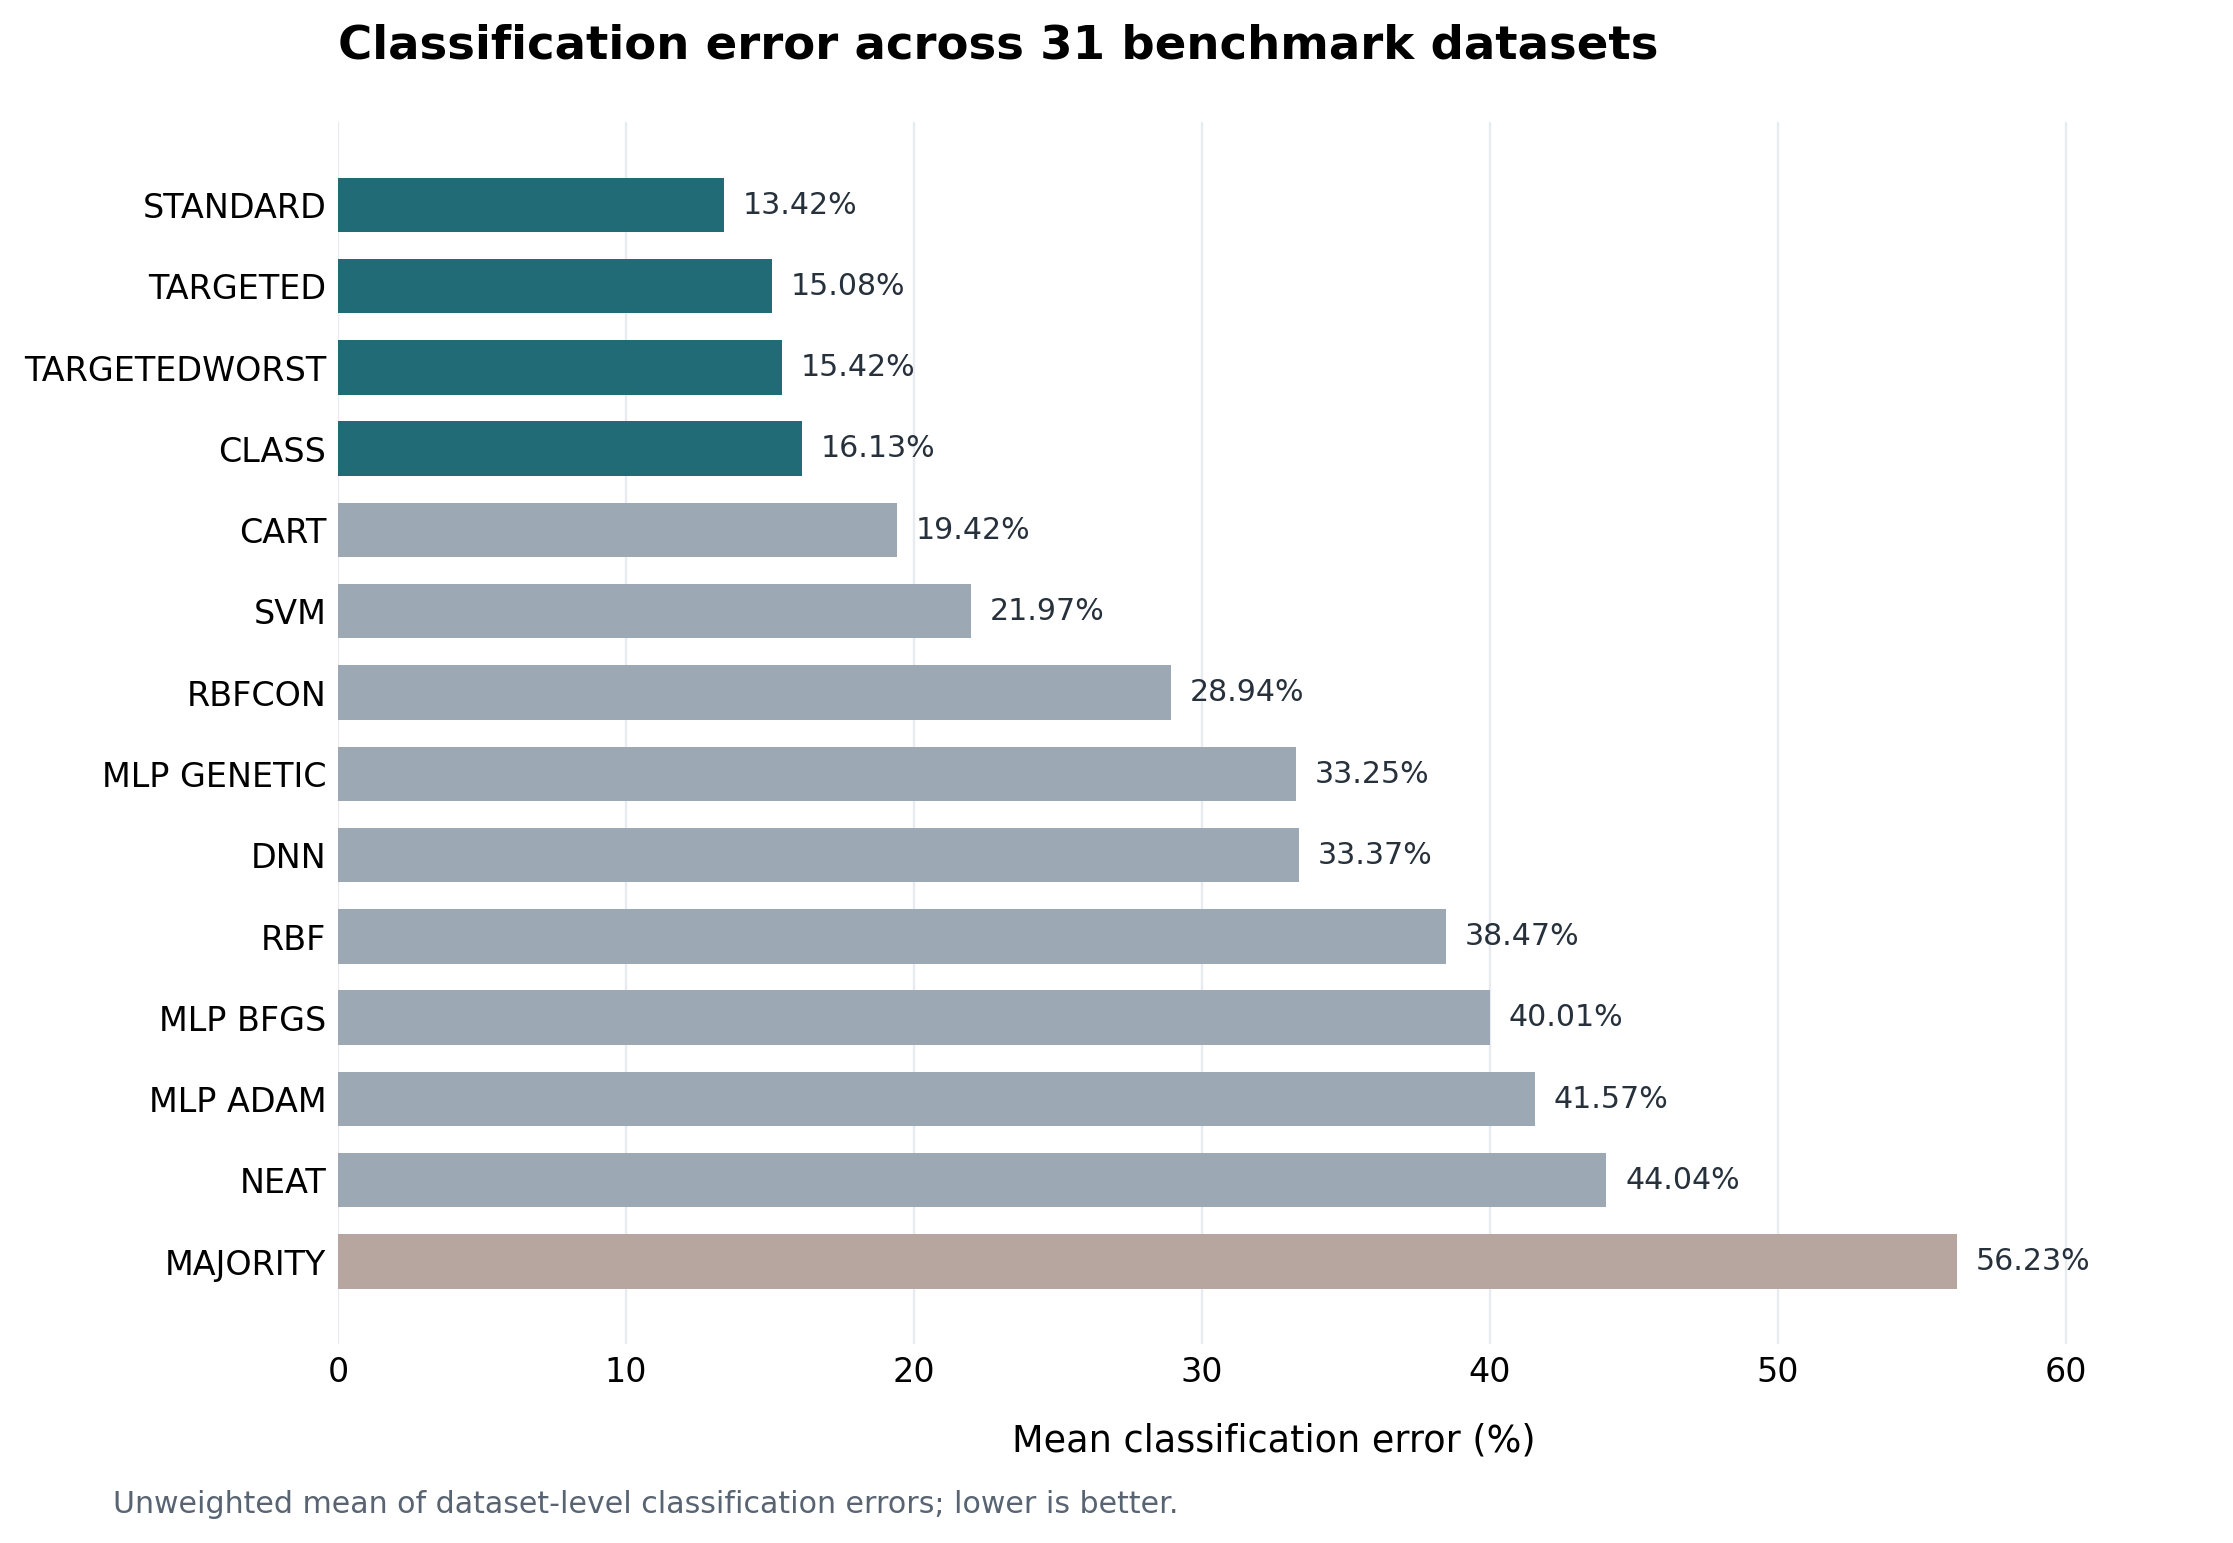
\includegraphics[scale=0.65]{majority_comparison}
\par\end{raggedright}
\caption{Average classification error (\%) of the evaluated classification
methods across 31 benchmark datasets. The reported values represent
the unweighted mean of the dataset-level classification errors. Lower
values indicate better classification performance. The majority-class
classifier is included as a simple reference baseline.\label{fig:majority}}

\end{figure}

To assess the influence of the additional computational effort introduced
by the crossover mechanism, we performed a supplementary comparison
between STANDARD and the original CLASS method under equal fitness
evaluation budgets. For each corresponding experimental run, the total
number of fitness evaluations performed by STANDARD was recorded and
subsequently used as the maximum evaluation budget for CLASS.

The results are presented in Table\textbf{ }\ref{tab:equal_budget}.
STANDARD achieved an average classification error of 13.71\%, compared
with 14.21\% for CLASS. Although STANDARD retained a small numerical
advantage, the difference was not statistically significant according
to the Wilcoxon signed-rank test ($p\approx0.608$).

These findings suggest that the additional computational effort associated
with the crossover mechanism may contribute to the improvements observed
in the original generation-based comparison. Nevertheless, the proposed
method maintains a slightly lower average classification error when
both approaches are evaluated under equal fitness evaluation budgets.

\begin{table}[htbp]
\centering
\caption{Classification error (\%) of STANDARD and CLASS
under equal fitness evaluation budgets.}
\label{tab:equal_budget}
\small
\begin{tabular}{|l|r|r|}
\hline
Dataset & STANDARD & CLASS-EQUAL \\
\hline
Alcohol      & \textbf{10.43} & 12.13 \\
Appendicitis & 15.00 & \textbf{14.00} \\
Beed         & \textbf{25.68} & 27.78 \\
Dermatology  & 6.00 & \textbf{5.14} \\
Gene         & 7.35 & \textbf{6.85} \\
Hayes-Roth   & 27.69 & \textbf{22.31} \\
Hepatitis    & \textbf{13.75} & 17.50 \\
Housevotes   & \textbf{3.48} & 3.89 \\
Ionosphere   & 10.00 & \textbf{7.43} \\
Lymography   & 24.29 & \textbf{22.86} \\
Nursery      & 19.10 & \textbf{18.41} \\
Optdigits    & \textbf{13.29} & 16.94 \\
Penbased     & \textbf{14.52} & 21.68 \\
Phoneme      & \textbf{16.73} & 17.54 \\
Pir          & 1.40 & \textbf{1.19} \\
Satimage     & 15.26 & \textbf{15.23} \\
Segment      & \textbf{9.05} & 10.35 \\
Shuttle      & 1.05 & \textbf{0.20} \\
Spambase     & \textbf{6.93} & 7.76 \\
Spiral       & \textbf{28.90} & 34.20 \\
Splice       & 7.21 & \textbf{6.90} \\
Student      & 7.45 & \textbf{5.73} \\
Texture      & \textbf{8.36} & 12.91 \\
Thyroid      & \textbf{0.64} & 0.96 \\
Twonorm      & 5.57 & \textbf{2.82} \\
Vehicle      & \textbf{35.83} & 36.07 \\
Wine         & 8.82 & 8.82 \\
Yeast        & 46.83 & \textbf{45.15} \\
Z\_F\_S       & \textbf{6.33} & 6.67 \\
Z\_O\_N\_F\_S & \textbf{25.40} & 28.80 \\
ZONF\_S      & 2.80 & \textbf{2.20} \\
\hline
\textbf{Mean} & \textbf{13.71} & 14.21 \\
\hline
\end{tabular}
\end{table}

To further examine whether the observed improvements can be attributed
to the proposed crossover mechanism rather than to the increased computational
budget, an additional experiment was conducted using a restart-based
baseline. In this experiment, the original CLASS method was executed
twice independently with different random seeds, without the additional
crossover mechanism. The total fitness evaluation budget was divided
between the two executions, and the best solution was selected according
to its training fitness. Consequently, the restart-based baseline
was allocated the same total number of fitness evaluations as STANDARD.

The results of the equal-budget comparison are summarized in Table
\ref{tab:evalBudgets}. As shown in the table, STANDARD achieved the
lowest average classification error (14.15\%), followed by MUTATION-LS
(14.22\%), equal-budget CLASS (14.53\%), and the restart-based baseline
(14.97\%). The restart-based approach outperformed STANDARD on 10
datasets, whereas STANDARD achieved lower classification errors on
18 datasets. The two methods produced identical results on one dataset.
A paired Wilcoxon signed-rank test yielded p-values of 0.1271 and
0.4118 for the comparisons of the restart-based approach against STANDARD
and equal-budget CLASS, respectively. Neither comparison revealed
a statistically significant difference at the 0.05 significance level.

\begin{table}[H]
\begin{centering}
\begin{tabular}{|c|c|}
\hline 
Method & Average classification error (\%)\tabularnewline
\hline 
\hline 
STANDARD-EQUAL & 14.15\%\tabularnewline
\hline 
MUTATION-LS & 14.22\%\tabularnewline
\hline 
CLASS-EQUAL & 14.53\%\tabularnewline
\hline 
CLASS-RESTART & 14.97\%\tabularnewline
\hline 
\end{tabular}
\par\end{centering}
\caption{Comparison of the average classification errors obtained by STANDARD-EQUAL,
MUTATION-LS, CLASS-EQUAL, and CLASS-RESTART under equal total fitness
evaluation budgets. \label{tab:evalBudgets}}

\end{table}

An additional statistical comparison was performed between STANDARD
and MUTATION-LS to investigate whether the proposed crossover mechanism
provides an advantage over mutation-based local search under the same
computational budget. MUTATION-LS achieved lower classification errors
on 11 datasets, whereas STANDARD performed better on 16 datasets,
with identical results observed on two datasets. The paired Wilcoxon
signed-rank test yielded a p-value of 0.6830, indicating that the
difference between the two methods was not statistically significant
at the 0.05 significance level.

The results of the computational-budget-controlled experiments indicate
that STANDARD achieved the lowest average classification error among
the four examined methods. However, the differences between STANDARD
and the restart-based baseline, as well as between STANDARD and MUTATION-LS,
were not statistically significant. These findings suggest that the
proposed crossover mechanism may offer a modest practical advantage
under equal computational budgets, but they do not establish its statistical
superiority over alternative strategies that allocate the same number
of fitness evaluations. Consequently, the improvements observed in
the main experimental evaluation should be interpreted in conjunction
with these additional controlled comparisons.

\textbf{Statistical analysis.} The comparison of the methods was based
on the average classification error of each method on each dataset,
so that every dataset provides one observation and $N=31$ observations
are available for each method. All tests were performed at the significance
level $\alpha=0.05$. For every table, the Friedman test was first
applied in order to examine the hypothesis that all the methods of
the table perform equally. For each dataset the methods are ranked
from the lowest to the highest error, with ties receiving the average
rank, and the test compares the mean ranks of the methods. The result
is also reported with the Iman-Davenport correction, which is less
conservative, and the strength of the differences is expressed by
Kendall's coefficient of concordance $W=\chi^{2}/(N(k-1))$, where
$k$ is the number of methods. The Nemenyi test was then used to compare
all the methods through their mean ranks, and two methods are considered
different when their mean ranks differ by more than the critical difference
$CD$. In addition, specific pairs of methods were compared with the
two-sided Wilcoxon signed-rank test for paired samples, applied to
the differences of the errors on the individual datasets, where zero
differences are discarded and tied absolute differences receive average
ranks. The p-values of the Wilcoxon tests were adjusted with the Holm
method separately for each table, over the family of comparisons of
that table. These are the ten comparisons of STANDARD with each of
the other methods in Table \ref{tab:methods_comparison}, and all
the pairs of methods in Table $\ref{tab:crossover_strategies}$ (three
comparisons) and in Table $\ref{tab:diff_NK}$ (six comparisons).
Finally, for Table $\ref{tab:diff_NK}$, the one-sided Page trend
test was used to examine whether the error decreases as $N_{K}$ increases,
together with the Spearman correlation between $N_{K}$ and the error
in each dataset, whose sign was summarized with a sign test.

Table \ref{tab:methods_comparison} presents the classification errors
obtained by STANDARD, the original GenClass method (CLASS), and the
additional classification methods considered in this study across
the 31 datasets. Lower values indicate better classification performance.
STANDARD achieved an average classification error of 13.42\%, compared
with 16.13\% for CLASS, corresponding to a reduction of 2.71 percentage
points (approximately 16.8\% relative reduction). Among the external
reference methods, the lowest average errors were obtained by CART
(19.42\%), SVM (21.97\%), and RBFCON (28.94\%), while the remaining
neural network methods ranged from 33.25\% (GEN) to 44.04\% (NEAT).
STANDARD obtained the lowest error on 19 of the 31 datasets, followed
by SVM (5 datasets), CART (3), GEN (2), RBF (1), and RBFCON (1), whereas
CLASS did not obtain the lowest error on any dataset. These findings
provide evidence of improved classification performance within the
GenClass framework under the examined experimental configuration.
The remaining classifiers are included as external reference methods,
rather than as part of an exhaustive comparison of supervised learning
algorithms.

The critical difference of the Nemenyi test is $CD=\frac{q_{\alpha}}{\sqrt{2}}\sqrt{\frac{k(k+1)}{6N}}$,
where $q_{\alpha}$ is the critical value of the studentized range
distribution for $k$ methods, and it therefore depends on the number
of methods compared. For each pair of methods, the size of the difference
was estimated with the Hodges-Lehmann estimator, which is the median
of the pairwise averages of the paired differences of the errors,
and its 95\% confidence interval was derived from the Wilcoxon signed-rank
test using the normal approximation. The effect size of each Wilcoxon
test was expressed as $r=Z/\sqrt{n}$, where $Z$ is the standardized
statistic of the test and $n$ is the number of datasets with non-zero
difference. The confidence intervals of the mean rank and of the mean
change in error in Figure $\ref{fig:effect_of_NK}$ were computed
with the percentile bootstrap, using 10,000 resamples of the datasets
with replacement. 

\medskip{}

{\small\textit{Notation for Figures $\ref{fig:standart_vs_others}$,
$\ref{fig:crossover_strategies}$ and $\ref{fig:effect_of_NK}$. Each
figure has four panels and a header with the Friedman test, the Iman-Davenport
correction and Kendall's $W$.}}{\small\par}
\begin{itemize}
\item {\small\textit{Box plots (top left): The box is the interquartile
range ($IQR$), the thick line is the median, the whiskers extend
up to $1.5\times IQR$, the diamond is the mean, the dots are the
datasets and the grey lines join the same dataset.}}{\small\par}
\item {\small\textit{Pairs \textquotedbl A vs B\textquotedbl{} (top right):
A is the first method named and B the second. The dot is the Hodges-Lehmann
median paired difference, error(B) \textminus{} error(A), with its
95\% confidence interval. Right of the dashed line, A has lower error.
The label gives the significance stars of the Holm-adjusted Wilcoxon
test and the wins/ties/losses of A.}}{\small\par}
\item {\small\textit{Mean ranks (bottom left): Mean Friedman rank (1 = best)
$\pm CD/2$, where $CD$ is the Nemenyi critical difference. Non-overlapping
bars differ at $\alpha=0.05$.}}{\small\par}
\item {\small\textit{Bottom right: In Figures $\ref{fig:standart_vs_others}$
and $\ref{fig:crossover_strategies}$,the distribution of error(B)
\textminus{} error(A) over the datasets for each pair (blue: A better,
red: B better). In Figure $\ref{fig:effect_of_NK}$,the mean change
in error relative to $N_{K}=2$ (upper) and the mean rank (lower)
as a function of $N_{K}$, with bootstrap 95\% confidence intervals.}}{\small\par}
\item {\small\textit{Stars: {*}{*}{*} $p<0.001$, {*}{*} $p<0.01$, {*}
$p<0.05$, ns = not significant (Holm-adjusted).}}{\small\par}
\end{itemize}
The statistical analysis of Table \ref{tab:methods_comparison} is
summarized in Figure \ref{fig:standart_vs_others}. The Friedman test
rejects the hypothesis that all eleven methods perform equally ($\chi^{2}(10)=164.49$,
$p=3.8\times10^{-30}$), a result confirmed by the Iman-Davenport
correction ($F(10,300)=33.91$, $p=9.9\times10^{-44}$), with a substantial
effect size (Kendall’s $W=0.53$). STANDARD obtains the best mean
rank (1.87), followed by CLASS (2.97), CART (3.90) and SVM (4.73),
while all the other methods have mean ranks above 5.5. In the paired
comparisons, STANDARD has lower error than every other method, with
Holm-adjusted Wilcoxon signed-rank p-values between$1.2\times10^{-5}$
and $1.0\times10^{-4}$ and wins in 25 to 31 of the 31 datasets. The
Hodges-Lehmann estimates of the median paired difference range from
approximately 2.4 percentage points (CLASS) to 30.4 percentage points
(NEAT), with 5.2 percentage points against CART and 8.0 percentage
points against SVM. None of the 95\% confidence intervals includes
zero, and the effect sizes are large ($r\geq0.72$, where values around
0.5 or above are conventionally considered large). The comparisons
with CLASS and CART require a careful reading. Their bars overlap
with that of STANDARD in the mean-rank panel, which means that the
conservative Nemenyi test does not separate them from STANDARD, since
the differences in mean rank (1.10 and 2.03) are smaller than the
critical difference (2.71). The paired Wilcoxon test, which also takes
into account the magnitude of the differences, nevertheless detects
a consistent improvement (28 wins and 3 losses against CLASS, 26 wins
and 5 losses against CART). STANDARD is worse than CLASS only on IONOSPHERE,
NURSERY and SHUTTLE, and worse than CART on NURSERY, PIRVISION, SHUTTLE,
Z\_F\_S and ZONF\_S. The competitor with the most individual wins
against STANDARD is SVM, which achieves lower error on six datasets
(IONOSPHERE, PIRVISION, SATIMAGE, SHUTTLE, STUDENT and TWONORM), although
the overall difference remains significant in favor of STANDARD (25
wins and 6 losses).

\begin{figure}[H]
\begin{centering}
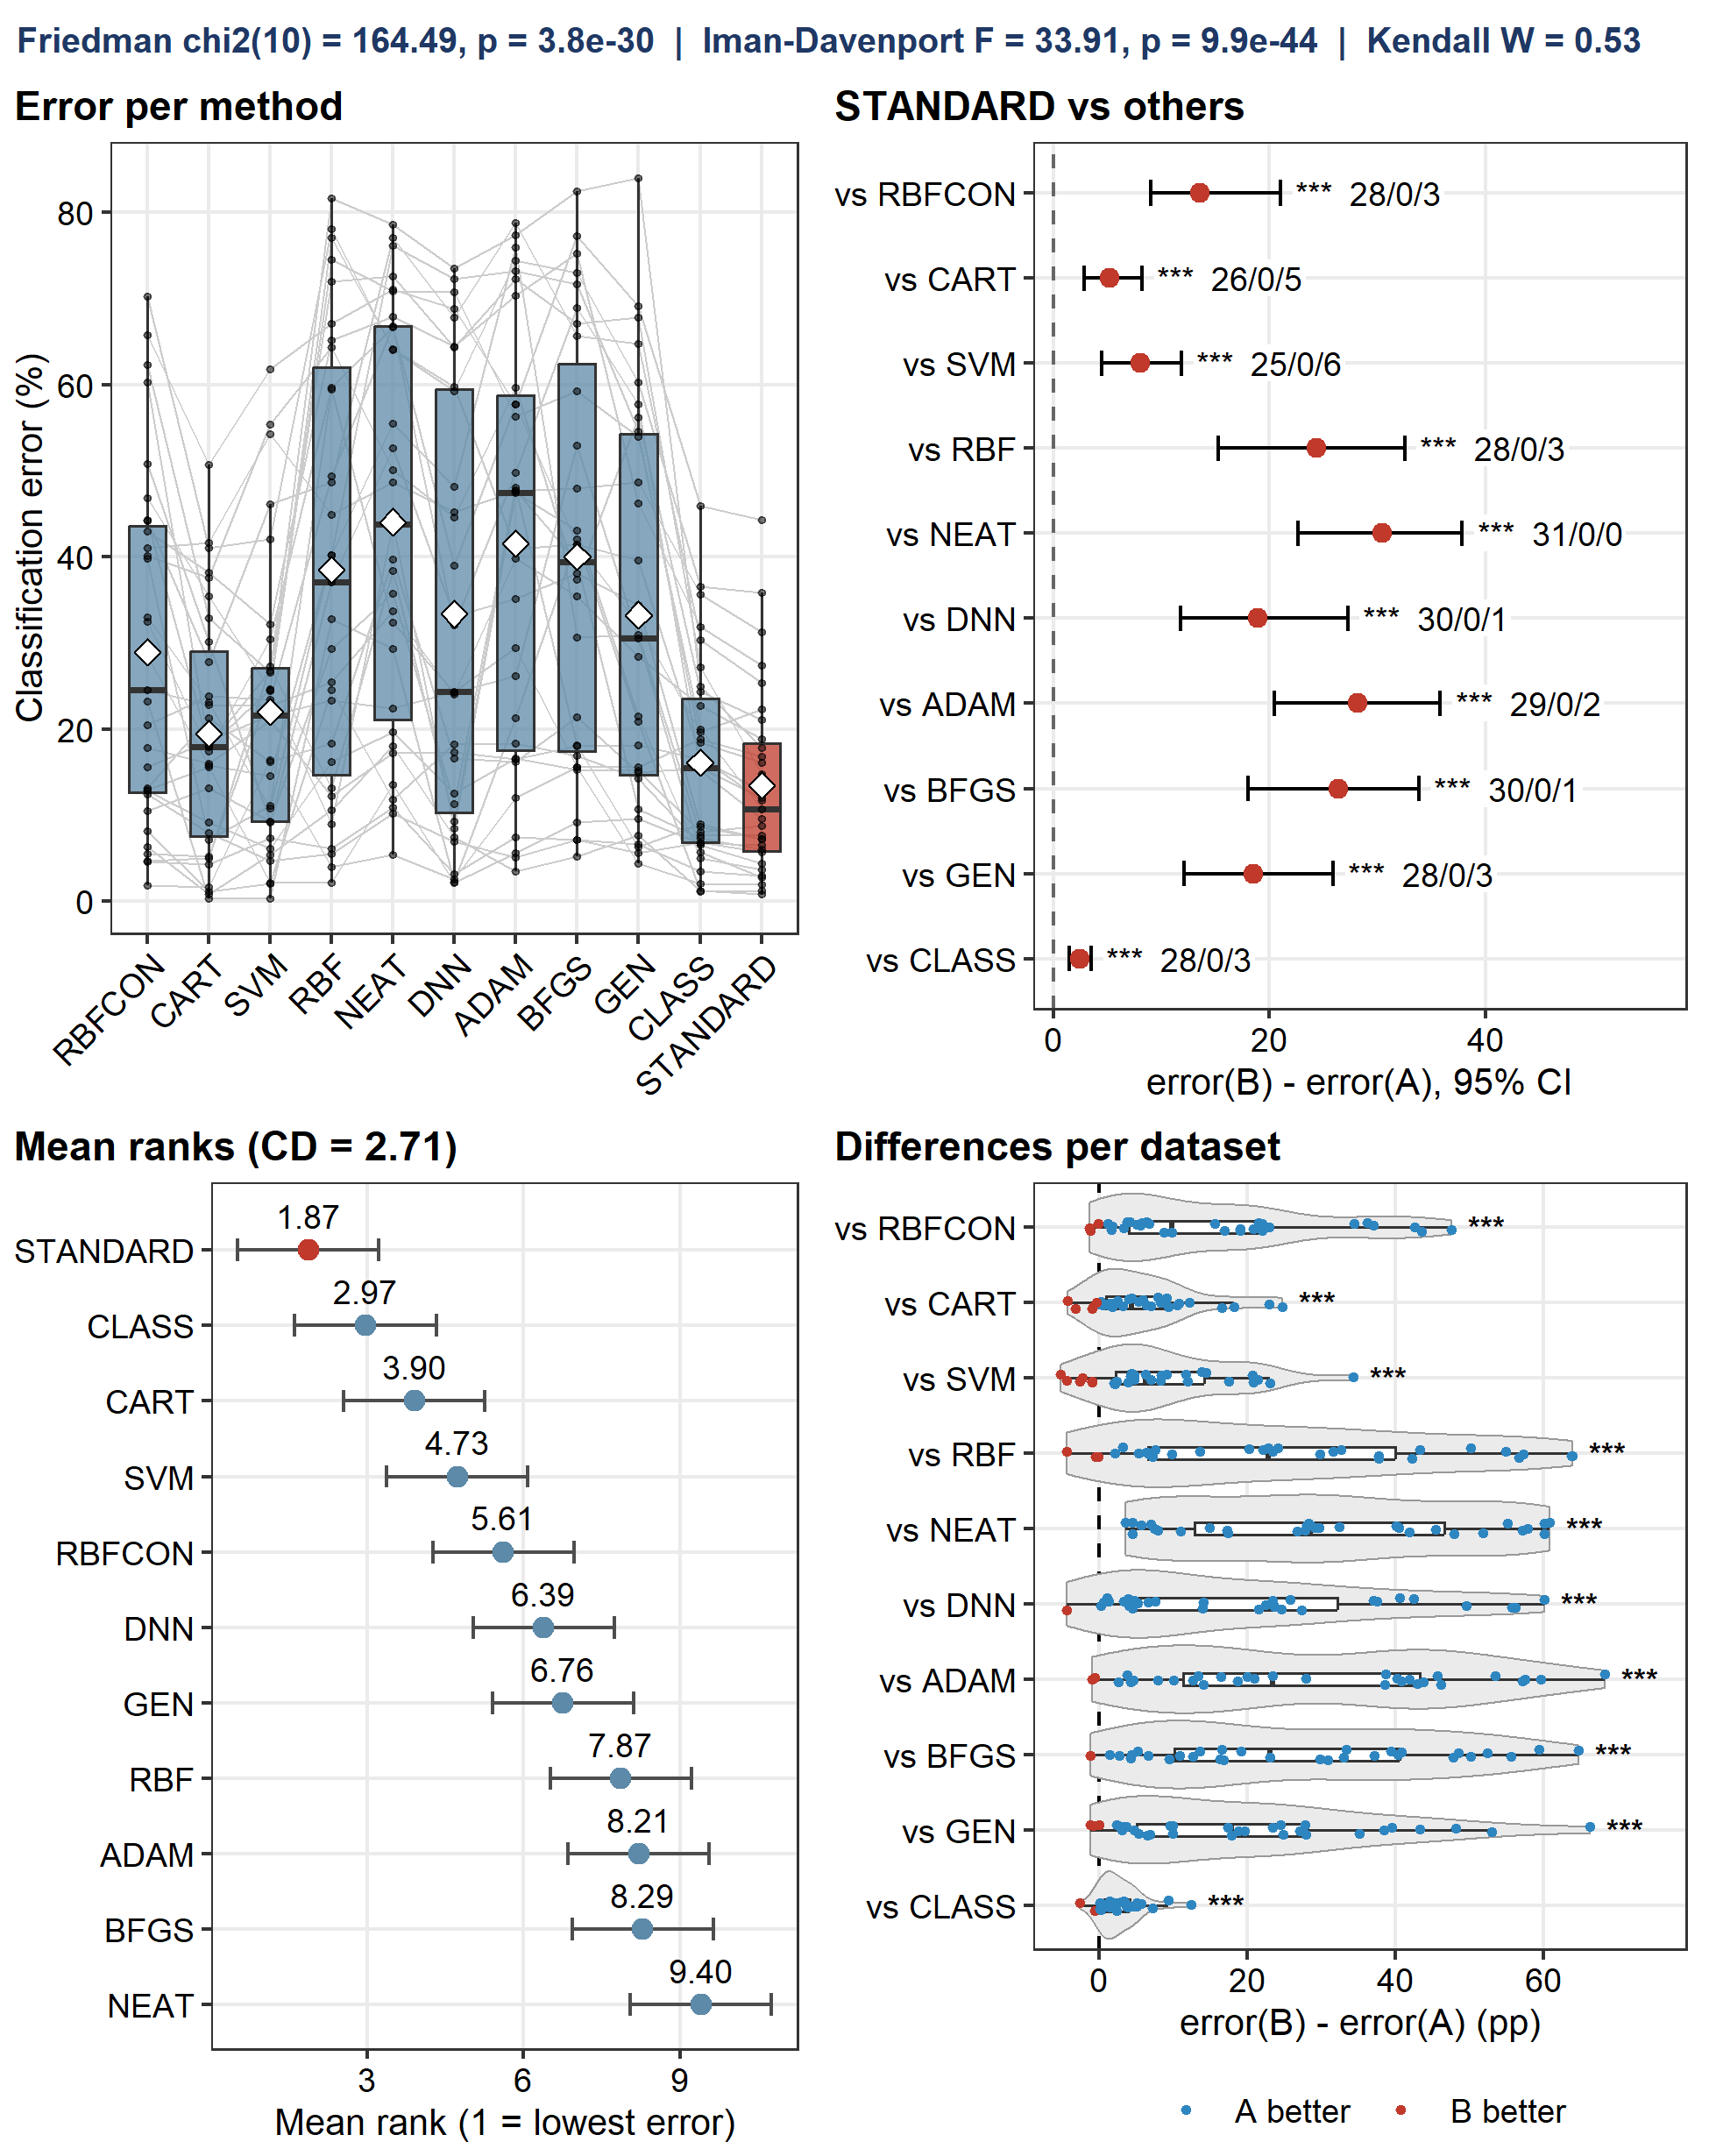
\includegraphics[scale=0.85]{tbl3_summary}
\par\end{centering}
\caption{Statistical comparison of the proposed method (STANDARD) against the
other classifiers over 31 datasets.\label{fig:standart_vs_others}}
\end{figure}

To examine the potential influence of dependent benchmark datasets,
an additional statistical analysis was conducted by excluding the
four EEG-derived datasets, which originate from the same underlying
recordings. The Wilcoxon signed-rank test was applied to the remaining
27 datasets. The STANDARD method retained a statistically significant
advantage over CLASS $\left(p=0.54\times10^{-6}\right)$. In contrast,
the differences between TARGETED and CLASS ($p=0.11105$) and between
TARGETEDWORST and CLASS ($p=0.04215$) were not statistically significant
after applying the Holm correction for multiple comparisons. These
findings indicate that the statistically significant improvement of
STANDARD over the original GenClass method persists after excluding
the related EEG datasets, whereas the evidence supporting improvements
from the other two crossover strategies is less conclusive.

\subsection{Crossover methods }

Table \ref{tab:crossover_strategies} isolates the effect of the crossover
strategy. STANDARD, in which the exchanged chromosome regions are
selected purely stochastically, achieves the lowest average error
(13.42\%), whereas the two strategies that exploit information collected
during the evolutionary process are less effective, with 15.08\% for
TARGETED and 15.42\% for TARGETEDWORST. STANDARD obtained the lowest
error in 24 of the 31 datasets, compared with 5 for TARGETED and 3
for TARGETEDWORST (a tie between the two targeted strategies in IONOSPHERE
is counted for both). The average gain of STANDARD is 1.66 percentage
points over TARGETED and 2.0 percentage points over TARGETEDWORST,
which correspond to relative reductions of 11.0\% and 13.0\%, respectively.
The two targeted strategies differ little from each other. Hence,
in these experiments, guiding the exchange of genetic material with
information from the evolutionary process did not improve upon the
purely random exchange.

\begin{table}[H]
\caption{Classification error (\%) of the three crossover strategies.\label{tab:crossover_strategies}}

\centering{}%
\begin{tabular}{|c|c|c|c|}
\hline 
DATASET & STANDARD & TARGETED & TARGETEDWORST\tabularnewline
\hline 
\hline 
ALCOHOL & 11.70\% & 17.65\% & 14.04\%\tabularnewline
\hline 
APPENDICITIS & 12.80\% & 16.40\% & 15.40\%\tabularnewline
\hline 
BEED & 27.45\% & 29.48\% & 31.93\%\tabularnewline
\hline 
DERMATOLOGY & 2.80\% & 6.12\% & 5.14\%\tabularnewline
\hline 
GENE & 7.29\% & 9.05\% & 8.20\%\tabularnewline
\hline 
HAYES ROTH & 21.08\% & 22.00\% & 25.38\%\tabularnewline
\hline 
HEPATITIS & 12.00\% & 16.25\% & 16.25\%\tabularnewline
\hline 
HOUSEVOTES & 2.96\% & 3.72\% & 3.04\%\tabularnewline
\hline 
IONOSPHERE & 8.74\% & 7.77\% & 7.77\%\tabularnewline
\hline 
LYMPHOGRAPHY & 18.86\% & 25.00\% & 21.86\%\tabularnewline
\hline 
NURSERY & 22.27\% & 21.44\% & 21.02\%\tabularnewline
\hline 
OPTDIGITS & 14.77\% & 19.59\% & 19.88\%\tabularnewline
\hline 
PENBASED & 17.79\% & 15.10\% & 23.85\%\tabularnewline
\hline 
PHONEME & 16.82\% & 17.86\% & 17.86\%\tabularnewline
\hline 
PIRVISION & 4.38\% & 4.47\% & 6.53\%\tabularnewline
\hline 
SATIMAGE & 16.14\% & 17.52\% & 18.14\%\tabularnewline
\hline 
SEGMENT & 9.57\% & 12.86\% & 11.26\%\tabularnewline
\hline 
SHUTTLE & 1.28\% & 1.35\% & 0.94\%\tabularnewline
\hline 
SPAMBASE & 7.28\% & 8.22\% & 8.10\%\tabularnewline
\hline 
SPIRAL & 31.25\% & 35.30\% & 34.83\%\tabularnewline
\hline 
SPLICE & 7.62\% & 8.12\% & 8.15\%\tabularnewline
\hline 
STUDENT & 5.72\% & 5.92\% & 6.45\%\tabularnewline
\hline 
TEXTURE & 10.71\% & 17.23\% & 16.59\%\tabularnewline
\hline 
THYROID & 0.83\% & 1.35\% & 1.53\%\tabularnewline
\hline 
TWONORM & 6.57\% & 3.90\% & 5.00\%\tabularnewline
\hline 
VEHICLE & 35.83\% & 39.64\% & 37.03\%\tabularnewline
\hline 
YEAST & 44.35\% & 45.22\% & 47.77\%\tabularnewline
\hline 
Z\_F\_S & 6.00\% & 6.40\% & 7.33\%\tabularnewline
\hline 
Z\_O\_N\_F\_S & 25.32\% & 28.12\% & 30.66\%\tabularnewline
\hline 
ZO\_NF\_S & 3.69\% & 3.08\% & 4.04\%\tabularnewline
\hline 
ZONF\_S & 2.00\% & 1.28\% & 2.04\%\tabularnewline
\hline 
\textbf{AVERAGE} & \textbf{13.42\%} & \textbf{15.08\%} & \textbf{15.42\%}\tabularnewline
\hline 
\end{tabular}
\end{table}

Figure \ref{tab:crossover_strategies} presents the statistical analysis
of Table \ref{tab:crossover_strategies}. The Friedman test indicates
significant differences among the three strategies ($\chi^{2}(2)=22.13$,
$p=1.6\times10^{-5}$, Iman-Davenport $F(2,60)=16.65$, $p=1.8\times10^{-6}$),
with a moderate effect size ($W=0.36$). STANDARD has the best mean
rank (1.32), against 2.27 for TARGETED and 2.40 for TARGETEDWORST.
Since the critical difference is 0.60, the bar of STANDARD does not
overlap with those of the other two strategies, while the bars of
TARGETED and TARGETEDWORST overlap. The paired tests agree with this
picture. STANDARD is significantly better than TARGETED (25 wins and
6 losses, median difference 1.62 percentage points, 95\% CI $[0.58,2.55]$,
$p=0.0018$, $r=0.60$) and than TARGETEDWORST (27 wins and 4 losses,
median difference 1.93 percentage points, 95\% CI $[1.08,2.80]$,
$p=1.6\times10^{-4}$, $r=0.73$). On the contrary, TARGETED and TARGETEDWORST
cannot be distinguished (15 wins, 3 ties and 13 losses, median difference
approximately 0.1 percentage points, 95\% CI $[-0.48,0.95]$, $p=0.64$,
$r=0.09$).

\begin{figure}[H]
\begin{centering}
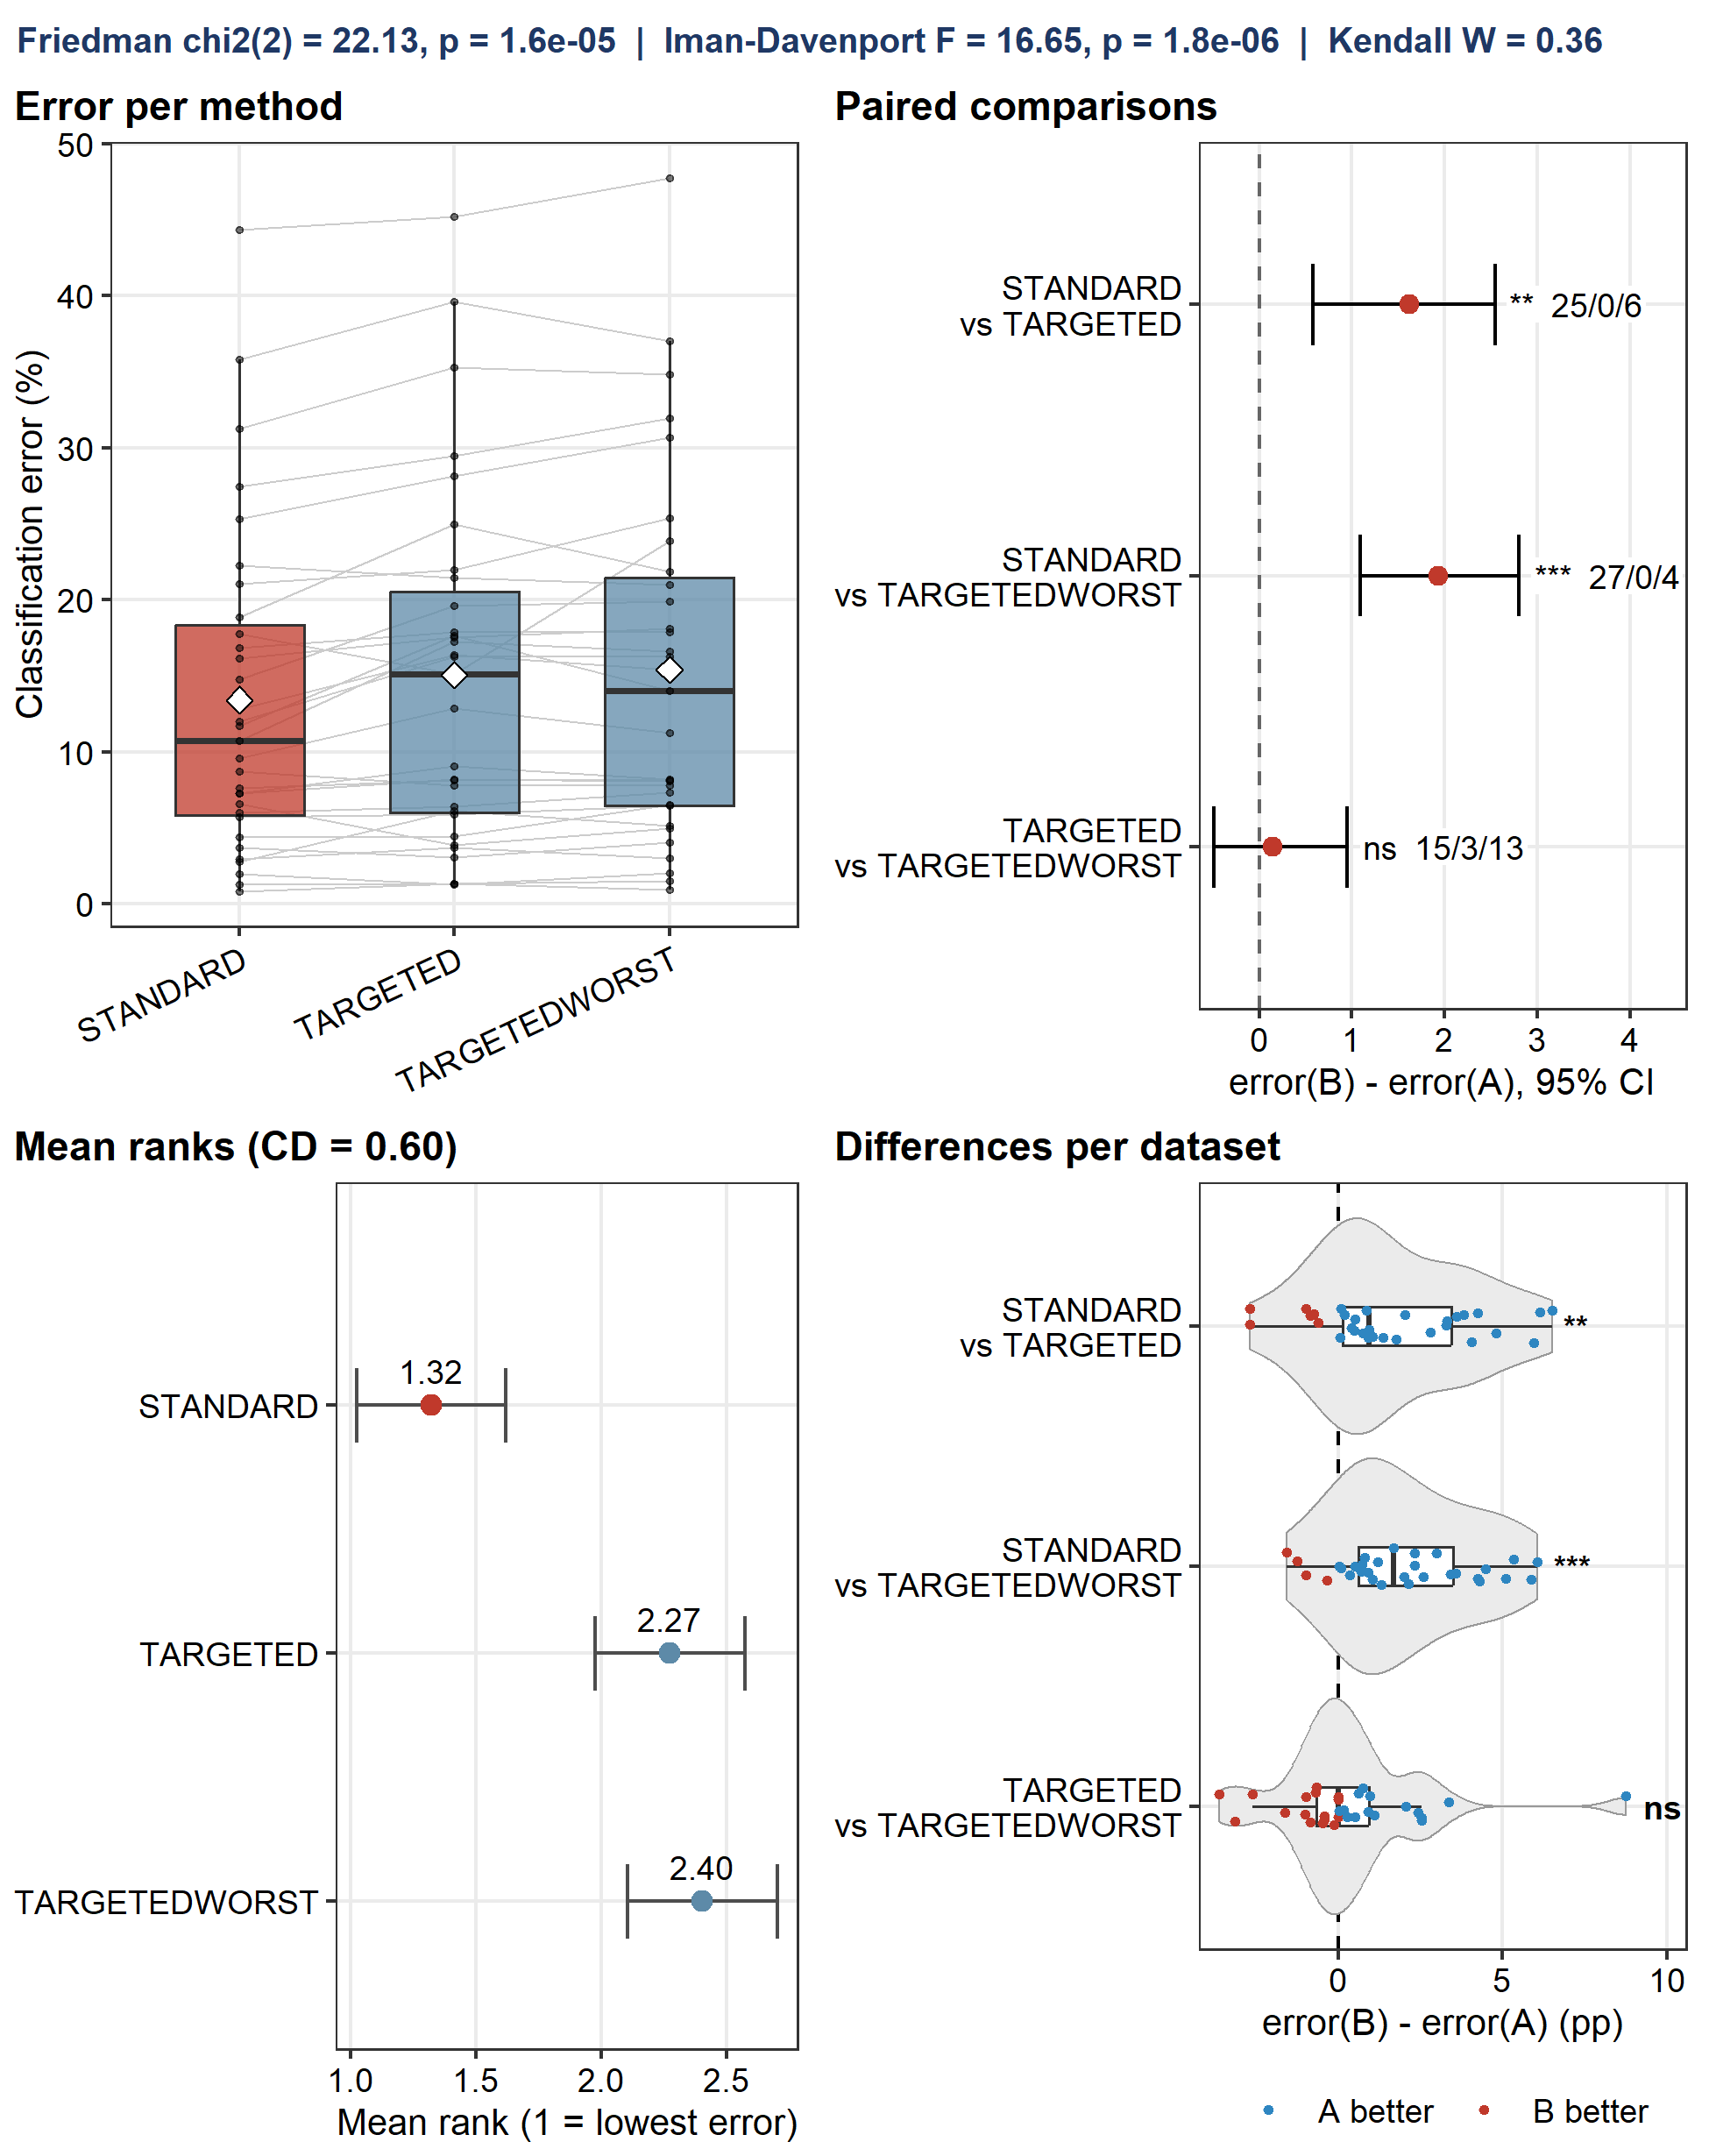
\includegraphics[scale=0.85]{tbl4_summary}
\par\end{centering}
\caption{Statistical comparison of the three crossover strategies. (STANDARD,
TARGETED, TARGETEDWORST).\label{fig:crossover_strategies}}
\end{figure}

To further assess the effectiveness of the three crossover strategies,
we performed pairwise comparisons against the original CLASS method
using two-sided Wilcoxon signed-rank tests. For the complete set of
31 datasets, the p-values were $1.381\times10^{-6}$ for STANDARD,
0.022385 for TARGETED, and 0.030285 for TARGETEDWORST. Since four
EEG-derived datasets originate from the same underlying recordings,
we additionally repeated the analysis after excluding these related
problems. For the remaining 27 datasets, the corresponding p-values
were $9.537\times10^{-6}$, 0.106917, and 0.040013, respectively.
After applying the Holm correction for the three comparisons, only
STANDARD retained statistical significance at the 0.05 level in the
analysis excluding the EEG-derived datasets. These findings indicate
that STANDARD provides the most robust improvement over the original
CLASS method, whereas the evidence supporting the two targeted strategies
is less conclusive.

\subsection{Number of crossing items}

The value $N_{K}=10$ was used as the default configuration in the
main experiments without performing a dataset-specific parameter optimization
procedure. The experiments presented in this subsection constitute
a sensitivity analysis intended to investigate the influence of the
number of chromosomes participating in the crossover operation. Although
$N_{K}=15$ achieved the lowest average classification error, the
default configuration was retained for the main comparisons rather
than selecting the best-performing value separately for each dataset.

Table \ref{tab:diff_NK} reports the results of the proposed method
when $N_{K}$=2, 5, 10 and 15 chromosomes participate in the crossover.
The column $N_{K}$=10 corresponds to the default value of Table \ref{tab:Values-for-the}
and coincides with the STANDARD column of Table \ref{tab:crossover_strategies}.
The average error decreases monotonically as $N_{K}$ increases, from
14.58\% for $N_{K}$=2 to 13.66\% for $N_{K}$=5, 13.42\% for $N_{K}$=10
and 13.19\% for $N_{K}$=15. The setting $N_{K}$=15 gave the lowest
error in 17 of the 31 datasets, $N_{K}$=5 and $N_{K}$=10 in 7 datasets
each, and $N_{K}$=2 in none. Increasing $N_{K}$ from 2 to 15 reduces
the average error by 1.39 percentage points, whereas each of the two
further increases beyond $N_{K}$=5 changes it by less than 0.3 percentage
points.

\begin{table}[H]
\caption{Experiments with the number that participate in the crossover procedure.\label{tab:diff_NK}}

\centering{}%
\begin{tabular}{|c|c|c|c|c|}
\hline 
DATASET & $N_{K}=2$ & $N_{K}=5$ & $N_{K}=10$ & $N_{K}=15$\tabularnewline
\hline 
\hline 
ALCOHOL & 12.55\% & 13.19\% & 11.70\% & 15.11\%\tabularnewline
\hline 
APPENDICITIS & 15.60\% & 14.40\% & 12.80\% & 15.80\%\tabularnewline
\hline 
BEED & 27.30\% & 26.78\% & 27.45\% & 25.47\%\tabularnewline
\hline 
DERMATOLOGY & 4.74\% & 4.86\% & 2.80\% & 4.00\%\tabularnewline
\hline 
GENE & 8.39\% & 7.29\% & 7.29\% & 6.91\%\tabularnewline
\hline 
HAYES ROTH & 20.77\% & 19.54\% & 21.08\% & 21.39\%\tabularnewline
\hline 
HEPATITIS & 14.00\% & 11.50\% & 12.00\% & 10.00\%\tabularnewline
\hline 
HOUSEVOTES & 3.63\% & 2.78\% & 2.96\% & 3.28\%\tabularnewline
\hline 
IONOSPHERE & 7.60\% & 7.31\% & 8.74\% & 8.80\%\tabularnewline
\hline 
LYMPHOGRAPHY & 23.71\% & 23.00\% & 18.86\% & 20.57\%\tabularnewline
\hline 
NURSERY & 20.33\% & 22.16\% & 22.27\% & 18.76\%\tabularnewline
\hline 
OPTDIGITS & 17.16\% & 14.56\% & 14.77\% & 13.99\%\tabularnewline
\hline 
PENBASED & 19.95\% & 16.54\% & 17.79\% & 14.22\%\tabularnewline
\hline 
PHONEME & 16.99\% & 16.21\% & 16.82\% & 16.00\%\tabularnewline
\hline 
PIRVISION & 8.49\% & 6.33\% & 4.38\% & 5.35\%\tabularnewline
\hline 
SATIMAGE & 15.91\% & 15.04\% & 16.14\% & 14.93\%\tabularnewline
\hline 
SEGMENT & 11.95\% & 9.91\% & 9.57\% & 9.44\%\tabularnewline
\hline 
SHUTTLE & 1.15\% & 0.62\% & 1.28\% & 0.24\%\tabularnewline
\hline 
SPAMBASE & 7.70\% & 7.98\% & 7.28\% & 7.33\%\tabularnewline
\hline 
SPIRAL & 36.80\% & 33.55\% & 31.25\% & 30.35\%\tabularnewline
\hline 
SPLICE & 7.46\% & 7.18\% & 7.62\% & 7.34\%\tabularnewline
\hline 
STUDENT & 6.11\% & 4.92\% & 5.72\% & 6.70\%\tabularnewline
\hline 
TEXTURE & 12.87\% & 12.73\% & 10.71\% & 12.44\%\tabularnewline
\hline 
THYROID & 1.57\% & 1.06\% & 0.83\% & 0.76\%\tabularnewline
\hline 
TWONORM & 5.62\% & 5.31\% & 6.57\% & 8.01\%\tabularnewline
\hline 
VEHICLE & 37.62\% & 34.81\% & 35.83\% & 33.69\%\tabularnewline
\hline 
YEAST & 46.21\% & 45.69\% & 44.35\% & 44.01\%\tabularnewline
\hline 
Z\_F\_S & 7.00\% & 6.47\% & 6.00\% & 5.67\%\tabularnewline
\hline 
Z\_O\_N\_F\_S & 27.28\% & 27.00\% & 25.32\% & 23.80\%\tabularnewline
\hline 
ZO\_NF\_S & 3.68\% & 3.32\% & 3.69\% & 3.40\%\tabularnewline
\hline 
ZONF\_S & 1.96\% & 1.44\% & 2.00\% & 1.16\%\tabularnewline
\hline 
\textbf{AVERAGE} & \textbf{14.58\%} & \textbf{13.66\%} & \textbf{13.42\%} & \textbf{13.19\%}\tabularnewline
\hline 
\end{tabular}
\end{table}

The identical results obtained by Targeted and TargetedWorst on the
Hepatitis and Phoneme datasets can be attributed to their binary classification
structure. In the proposed chromosome representation, a problem with
$C$ classes contains$C-1$ explicit classification rules, with the
remaining class handled by a default rule. Consequently, for binary
classification problems, the single explicit rule spans the entire
chromosome, making the class-specific crossover restriction of TargetedWorst
equivalent to the unrestricted selection employed by Targeted.

For the BEED dataset, the identical classification error reported
for CLASS and TargetedWorst (31.93\%) should not be interpreted as
algorithmic equivalence. BEED contains four classes, and TargetedWorst
performs additional class-directed crossover operations that are absent
from the CLASS baseline. Supplementary implementation checks confirmed
that these operations were executed and produced accepted fitness
improvements. However, the numerical coincidence in the original results
has not been independently reproduced.

Figure \ref{fig:effect_of_NK} presents the corresponding statistical
analysis. The Friedman test detects significant differences among
the four settings ($\chi^{2}(3)=21.97$, $p=6.6\times10^{-5}$, Iman-Davenport
$F(3,90)=9.28$, $p=2.1\times10^{-5}$), although with a smaller effect
size than in the previous comparisons ($W=0.24$). The mean rank is
the worst for $N_{K}=2$ (3.35) and the best for $N_{K}=15$ (1.87),
with $N_{K}=5$ (2.27) and $N_{K}=10$ (2.50) in between. The one-sided
Page trend test, which examines whether the error decreases as $N_{K}$
increases, confirms a significant trend ($z=4.08$, $p=2.3\times10^{-5}$).
In agreement, the Spearman correlation between $N_{K}$ and the error
is negative in 23 of the 29 datasets where it is non-zero (median
correlation $-0.6$, sign test $p=0.0023$). The pairwise comparisons
show, however, that this trend is mainly due to the weakness of the
smallest setting. The value $N_{K}=2$ has significantly higher error
than $N_{K}=5$ ($p=3.8\times10^{-4}$), $N_{K}=10$ ($p=0.0047$)
and $N_{K}=15$ ($p=0.0039$), with median differences of approximately
0.8, 1.0 and 1.3 percentage points, respectively. None of the differences
among $N_{K}=5$, 10 and 15 is statistically significant (adjusted
$p=0.61$ for 5 versus 10, 0.20 for 5 versus 15 and 0.61 for 10 versus
15), and their confidence intervals include zero. Therefore, a very
small number of chromosomes in the crossover is detrimental, whereas
beyond $N_{K}=5$ any further benefit is small and is not statistically
established in these experiments, although $N_{K}=15$ has the best
mean rank.

\begin{figure}[H]
\begin{centering}
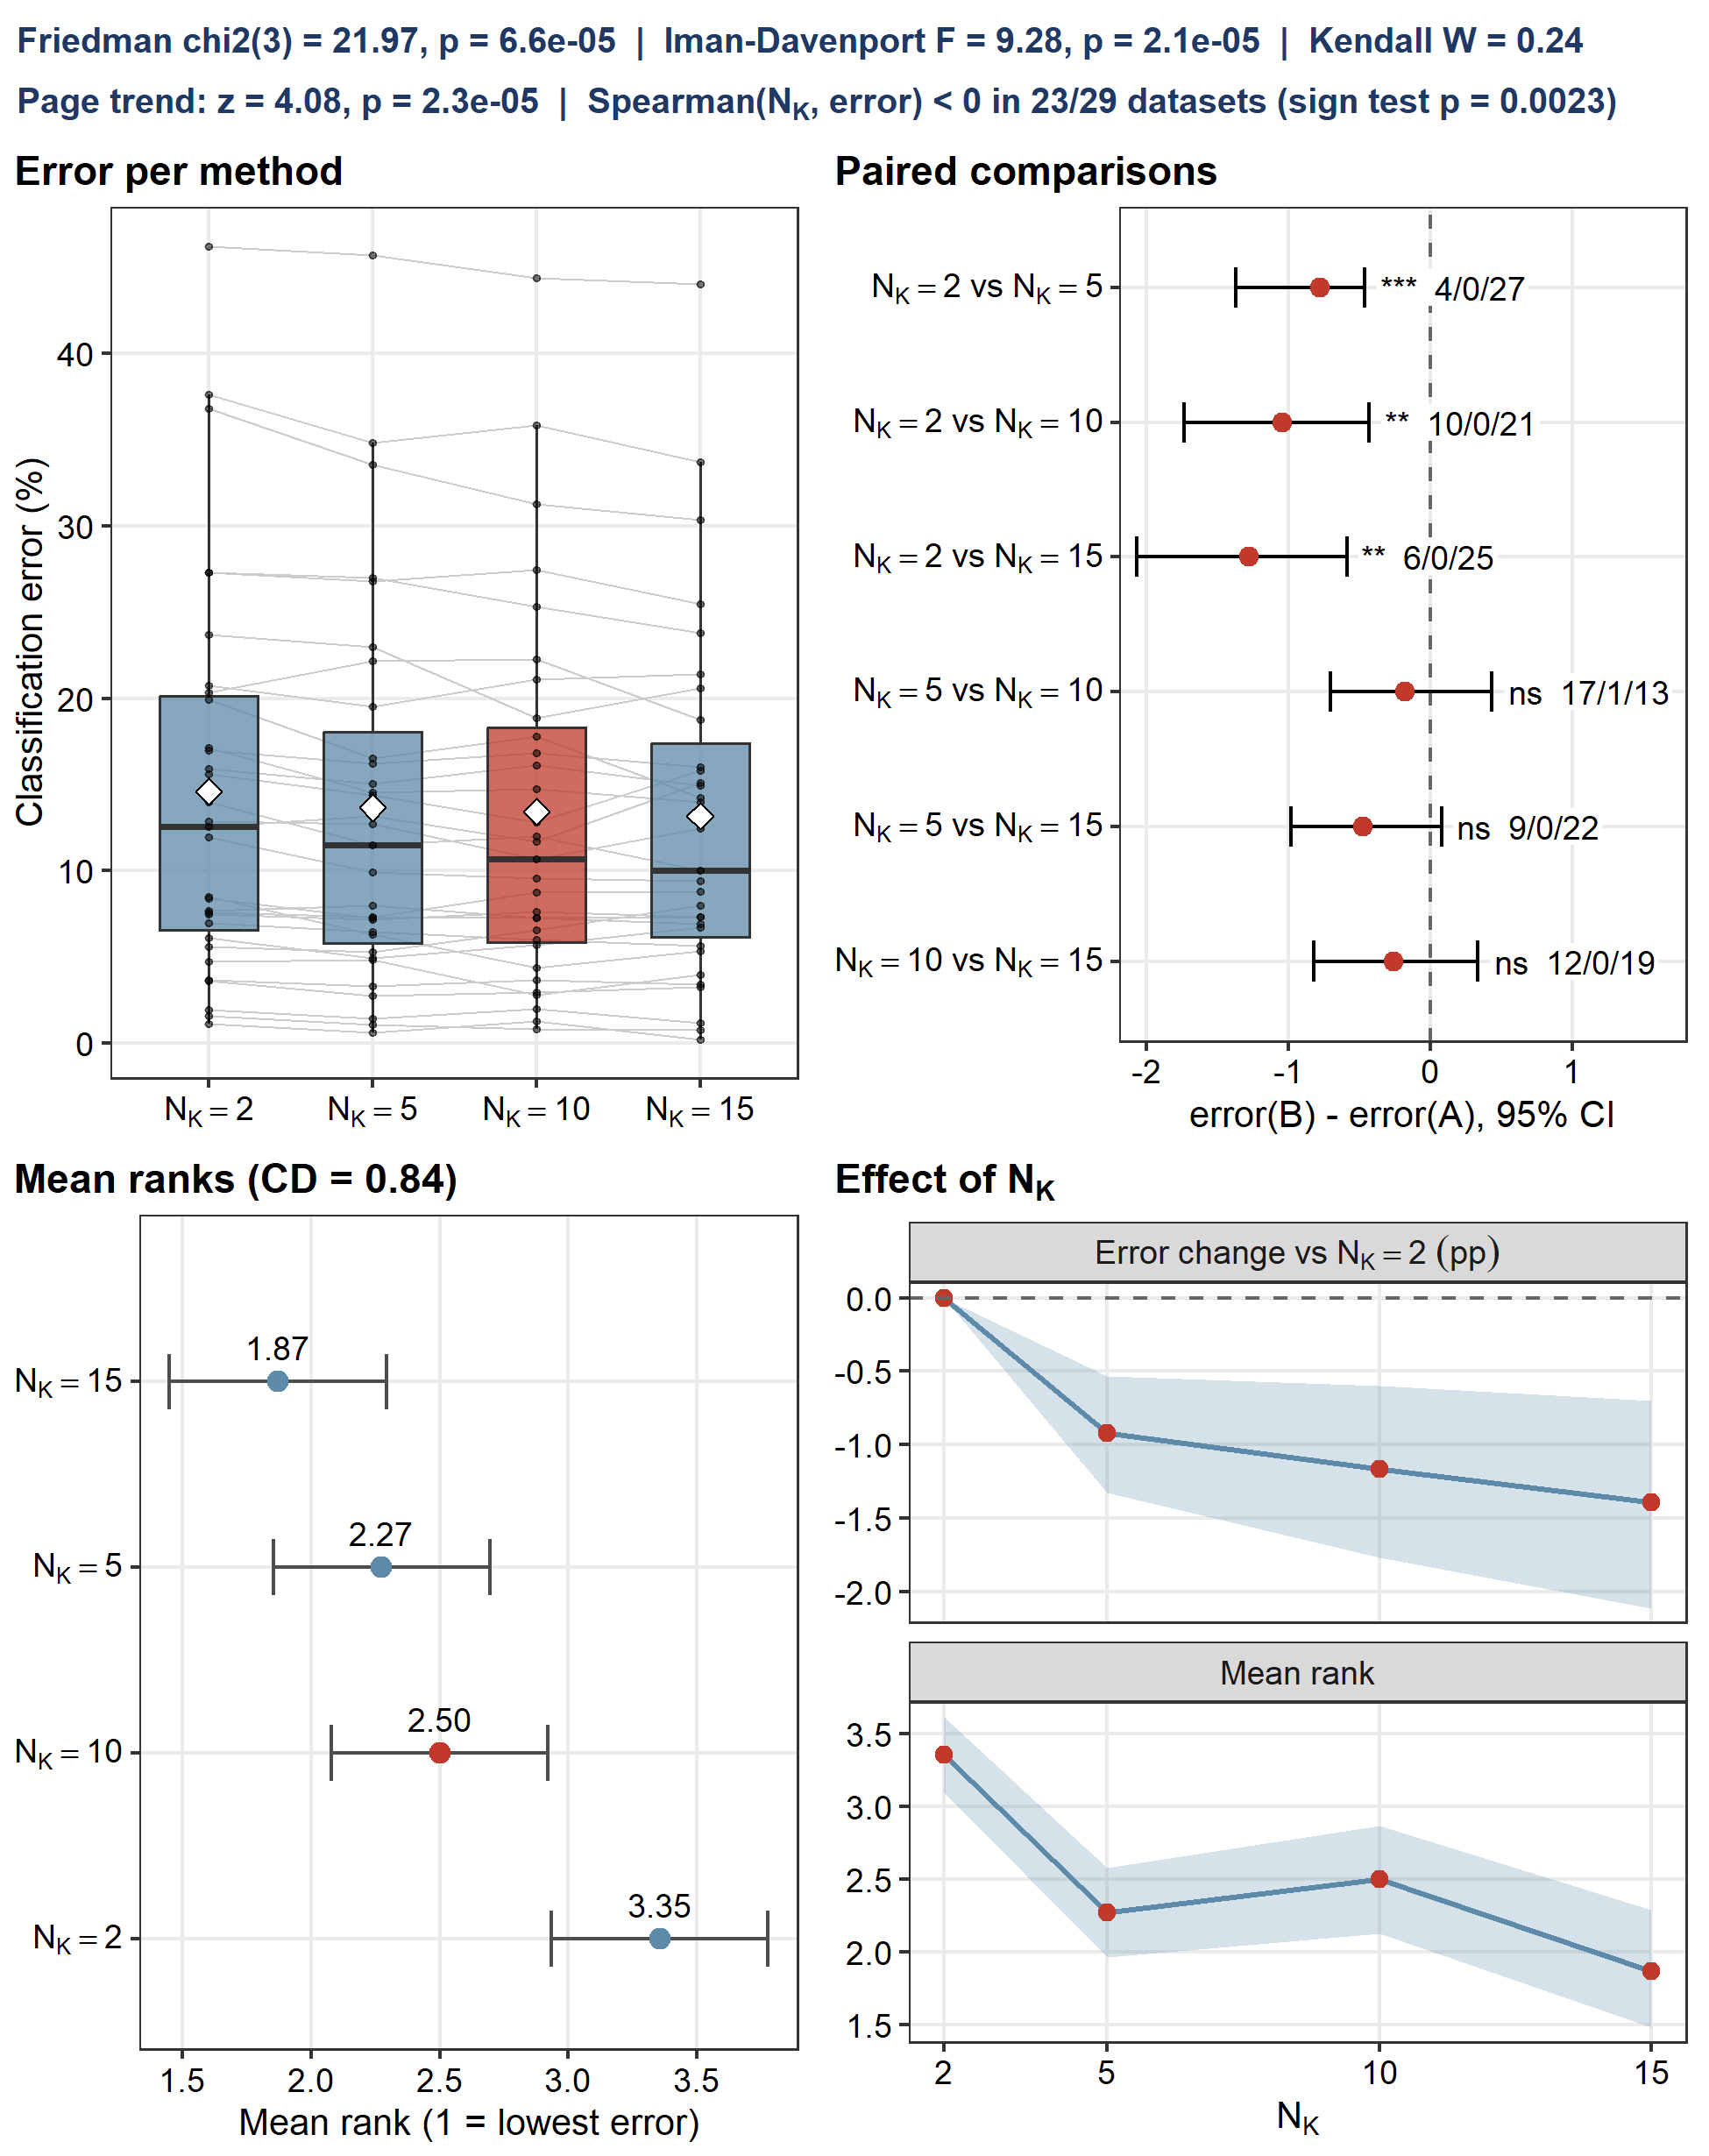
\includegraphics[scale=0.85]{tbl5_summary}
\par\end{centering}
\caption{Effect of the number of chromosomes ($N_{K}$) participating in the
crossover on the proposed method.\label{fig:effect_of_NK}}
\end{figure}
\begin{figure}[H]
\begin{centering}
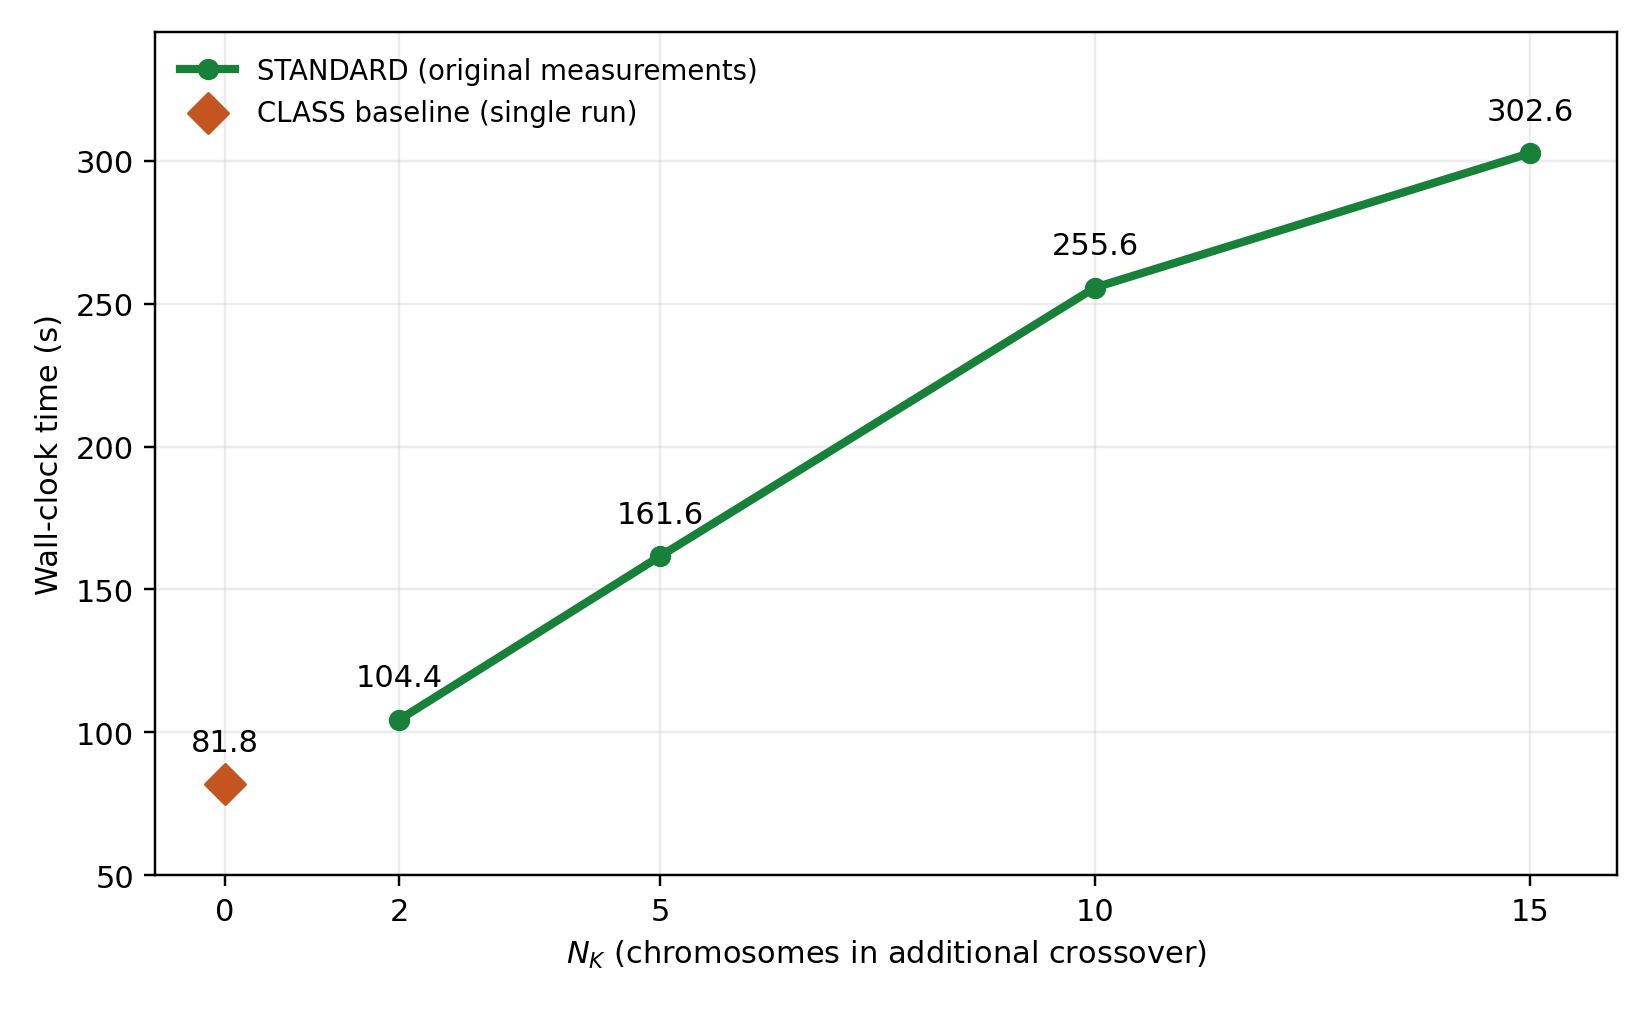
\includegraphics[scale=0.75]{time}
\par\end{centering}
\caption{Execution time of the STANDARD crossover technique on the Dermatology
dataset for different values of $(N_{K})$. The baseline configuration
$((N_{K}=0))$ required 81.80 seconds, while execution time increased
to 302.60 seconds for $(N_{K}=15)$. The baseline value represents
a single execution, whereas the remaining values correspond to the
previously reported average execution times. \label{fig:time_dermatology}}
\end{figure}

The figure shows the average execution time of the Standard technique
on the Dermatology dataset for $N_{K}$=2, 5, 10 and 15. The time
increases with$N_{K}$, from 104.4 s for $N_{K}=2$ to 302.6 s for
$N_{K}=15$, which is about 2.9 times higher. The increase is approximately
linear up to $N_{K}=10$, at about 19 s per additional chromosome,
and becomes slower from $N_{K}=10$ to $N_{K}=15$, at about 9 s per
additional chromosome. The observed execution-time increase is not
uniform across the examined values of $N_{K}$. Although the increase
becomes smaller between $N_{K}=10$ and $N_{K}=15$, the available
measurements do not establish the underlying cause of this behavior.
Consequently, no specific explanation for the change in the slope
of the execution-time curve can be confirmed from these results alone. 

For the Dermatology dataset, the default value $N_{K}=10$ requires
255.6 s, whereas $N_{K}=15$ requires 302.6 s, representing an increase
of approximately 18\%. This dataset is used solely to illustrate the
computational cost associated with increasing $N_{K}$ and should
not be considered representative of the overall classification performance.
Across all 31 datasets, $N_{K}=15$ achieves the lowest average classification
error and the best mean rank, although its advantage over $N_{K}=5$
and $N_{K}=10$ is not statistically significant after correction
for multiple comparisons.

\subsection{\textbf{Computational Cost Analysis}}

To provide a more comprehensive assessment of the computational cost
of the proposed crossover operators, additional experiments were conducted
on three relatively large datasets: Nursery, Pirvision, and Shuttle.
Both wall-clock execution time and the total number of fitness evaluations
were measured for the original CLASS configuration and the STANDARD,
TARGETED, and TARGETEDWORST crossover variants. All configurations
were evaluated using identical experimental settings and the same
random seed, with $N_{K}=0$ for CLASS and $N_{K}=10$ for the crossover
variants.

Table \ref{tab:computational_cost} reports the measured execution
times and total fitness evaluation counts. The results reveal substantial
differences in computational cost among the examined approaches. STANDARD
consistently exhibits the highest overhead, requiring approximately
3.49-{}-3.93 times the execution time of CLASS. In contrast, TARGETED
introduces a more moderate overhead, with execution-time ratios ranging
from 1.40 to 1.67. TARGETEDWORST exhibits dataset-dependent behavior,
with execution-time ratios ranging from 0.64 to 1.85.

The number of fitness evaluations generally follows a similar pattern,
although execution time is not strictly proportional to the evaluation
count. This suggests that factors beyond the number of evaluations
may also influence total execution time. In particular, STANDARD introduces
a substantial increase in both execution time and fitness evaluations.

An additional baseline measurement was performed on the Dermatology
dataset with $N_{K}=0$. The recorded execution time was 81.80 seconds,
with 2,041,800 fitness evaluations. The previously reported time of
255.60 seconds at $N_{K}=10$ is approximately 3.12 times this baseline;
this comparison is valid only if both measurements were obtained under
equivalent experimental conditions.

These findings demonstrate that the computational overhead of the
proposed crossover strategies depends on the operator and dataset
and can be substantial, particularly for STANDARD. The additional
crossover operations therefore represent a trade-off between classification
performance and computational cost rather than a computationally negligible
modification. Because these measurements correspond to a single execution
per configuration, they are intended to characterize computational
overhead rather than establish statistically significant timing differences.

% Computational cost comparison (single run per configuration).
% Requires \usepackage{booktabs} in the preamble.
\begin{table}[H]
\centering
\caption{Wall-clock execution time and total fitness evaluations for CLASS and the three crossover variants on Nursery, Pirvision, and Shuttle. The baseline uses $N_K=0$, while the crossover variants use $N_K=10$. Results correspond to one run per configuration.}
\label{tab:computational_cost}
\begin{tabular}{llrr}
\toprule
Dataset & Method & Time (s) & Fitness evaluations \\
\midrule
Nursery & CLASS & 1230.76 & 1595309 \\
        & STANDARD & 4293.11 & 5564200 \\
        & TARGETED & 1755.92 & 2038902 \\
        & TARGETEDWORST & 2275.75 & 2079594 \\
\midrule
Pirvision & CLASS & 1984.78 & 2072441 \\
          & STANDARD & 7805.84 & 6776246 \\
          & TARGETED & 2771.94 & 2676918 \\
          & TARGETEDWORST & 1267.48 & 2160418 \\
\midrule
Shuttle & CLASS & 4750.54 & 1783945 \\
        & STANDARD & 18632.64 & 6335527 \\
        & TARGETED & 7912.64 & 2481313 \\
        & TARGETEDWORST & 7386.76 & 2364263 \\
\bottomrule
\end{tabular}
\end{table}

\subsection{Crossover Ablation Study}

To examine whether the observed behavior of targeted crossover is
attributable to donor selection, exchange geometry, or local grammar-based
matching, we conducted a controlled ablation study. Six crossover
configurations were considered: 
\begin{enumerate}
\item \emph{Standard}, the original standard crossover using donors sampled
from the population and tail exchange; 
\item \emph{Standard+Elite}, which retains the standard exchange but restricts
donor selection to the top 20\% of the population; 
\item \emph{Standard+Block}, which retains population-wide donor selection
but limits the exchanged segment to at most 16 codons; 
\item \emph{Targeted}, which combines elite donor selection, a maximum
exchanged block length of 16 codons, and local grammar-based matching;
\item \emph{Targeted+Full}, which replaces elite donor selection in Targeted
with population-wide sampling; and 
\item \emph{TargetedWorst}, the corresponding targeted variant using its
alternative recipient-selection strategy. These controls examine individual
design choices but do not constitute a complete factorial isolation
of all possible interactions.
\end{enumerate}
Experiments used ten classification datasets (Dermatology, Hepatitis,
Housevotes, Ionosphere, Optdigits, Segment, Spambase, Thyroid, Vehicle,
and Yeast). For each dataset and configuration, 30 runs were performed
using the same set of random seed values, giving 1,800 runs in total.
All runs were constrained to exactly 100,000 fitness evaluations,
with a maximum of 1,000 generations. The number of crossover items
was 10; the targeted variants used 20 crossover iterations and a maximum
block length of 16 codons. The results refer to one predefined training/test
split per dataset, rather than a complete ten-fold cross-validation.
Consequently, the conclusions are conditional on the selected splits.
The recorded test classification errors are reported as mean $\pm$
sample standard deviation across the 30 runs.

\begin{table*}[t]
\centering
\caption{Classification error (\%, mean $\pm$ standard deviation over 30 runs) under an equal budget of 100,000 fitness evaluations per run. Lower values are better.}
\label{tab:crossover_ablation_error}
\scriptsize
\setlength{\tabcolsep}{3pt}
\begin{tabular}{lrrrrrr}
\hline
Dataset & Standard & Std.+Elite & Std.+Block & Targeted & Targeted+Full & TargetedWorst \\
\hline
Dermatology & $6.48\pm5.19$ & $10.67\pm6.75$ & $9.05\pm5.26$ & $6.86\pm5.49$ & $8.19\pm5.45$ & $7.24\pm5.02$ \\
Hepatitis & $21.25\pm16.46$ & $25.42\pm16.89$ & $16.25\pm13.19$ & $24.58\pm14.86$ & $22.50\pm15.19$ & $24.58\pm14.86$ \\
Housevotes & $4.06\pm1.10$ & $4.35\pm0.00$ & $4.20\pm0.79$ & $4.06\pm1.10$ & $3.48\pm1.77$ & $4.06\pm1.10$ \\
Ionosphere & $13.14\pm3.80$ & $13.71\pm4.34$ & $12.67\pm4.09$ & $11.52\pm3.71$ & $11.62\pm3.26$ & $11.52\pm3.71$ \\
Optdigits & $43.62\pm5.69$ & $44.86\pm5.00$ & $43.74\pm5.97$ & $43.14\pm5.01$ & $42.98\pm3.72$ & $46.36\pm4.69$ \\
Segment & $27.56\pm6.46$ & $29.60\pm6.06$ & $26.93\pm6.40$ & $25.57\pm4.85$ & $25.02\pm5.46$ & $25.32\pm7.19$ \\
Spambase & $10.09\pm2.12$ & $10.61\pm2.10$ & $9.51\pm2.25$ & $9.69\pm1.95$ & $8.69\pm1.84$ & $9.69\pm1.95$ \\
Thyroid & $4.79\pm1.61$ & $4.25\pm2.04$ & $5.00\pm1.64$ & $4.48\pm1.78$ & $3.51\pm1.78$ & $4.20\pm1.78$ \\
Vehicle & $39.29\pm5.99$ & $42.54\pm8.11$ & $42.78\pm7.84$ & $40.71\pm8.08$ & $39.64\pm6.12$ & $39.33\pm6.63$ \\
Yeast & $55.59\pm4.50$ & $57.18\pm4.03$ & $54.48\pm3.55$ & $54.84\pm3.70$ & $55.09\pm8.14$ & $53.81\pm4.33$ \\
\hline
\end{tabular}
\end{table*}

Table \ref{tab:crossover_ablation_error} shows that no single operator
is best on every dataset. Targeted+Full achieves the lowest mean classification
error on five datasets, while Standard performs best on Dermatology
and Standard+Block on Hepatitis. The relatively small differences
between several configurations should not be interpreted as evidence
of universal superiority.

\begin{table}[t]
\centering
\caption{Crossover statistics aggregated over all ten datasets and 30 runs per dataset. Accepted improvements and skipped trials are mean counts per run; the last column is the ratio of total accepted improvements to total crossover fitness evaluations, multiplied by 1,000.}
\label{tab:crossover_ablation_efficiency}
\scriptsize
\begin{tabular}{lrrr}
\hline
Operator & Accepted/run & Skipped/run & Accepted/1,000 evals \\
\hline
Standard & 965.5 & 0.0 & 12.18 \\
Standard+Elite & 810.0 & 0.0 & 10.22 \\
Standard+Block & 904.0 & 0.0 & 11.40 \\
Targeted & 629.8 & 489.2 & 29.33 \\
Targeted+Full & 636.1 & 560.7 & 29.67 \\
TargetedWorst & 479.8 & 1355.1 & 23.06 \\
\hline
\end{tabular}
\end{table}

As shown in Table \ref{tab:crossover_ablation_efficiency}, the targeted
configurations produce more accepted improvements per crossover fitness
evaluation than the standard configurations. In particular, Targeted
yields approximately 2.41 times the normalized acceptance count of
Standard. However, these are not equal numbers of crossover evaluations:
the fixed total evaluation budget also covers other algorithmic operations,
and the crossover implementations use different numbers of trials
and evaluations. The normalized ratio is therefore an operational
efficiency measure, not direct proof that grammar-based matching alone
causes the difference. TargetedWorst also records substantially more
skipped trials, indicating that some attempted operations terminate
without a crossover fitness evaluation.

For a dataset-level statistical comparison, the six operators were
ranked according to their mean classification error on each of the
ten datasets. A Friedman test identified an overall difference ($\chi^{2}(5)=18.878$,
$p=0.00203$). The mean ranks (smaller is better) were 2.20 for Targeted+Full,
2.85 for TargetedWorst, 3.05 for Targeted, 3.50 for Standard, 3.90
for Standard+Block, and 5.50 for Standard+Elite. Five pre-specified
pairwise comparisons were subsequently performed using two-sided Wilcoxon
signed-rank tests on the ten paired dataset means, with Holm correction:
Standard versus Targeted ($p_{\mathrm{adj}}=1.0000$), Standard versus
Standard+Elite ($p_{\mathrm{adj}}=0.0488$), Standard versus Standard+Block
($p_{\mathrm{adj}}=1.0000$), Targeted versus Targeted+Full ($p_{\mathrm{adj}}=0.6406$),
and Targeted versus TargetedWorst ($p_{\mathrm{adj}}=1.0000$). Only
the Standard versus Standard+Elite comparison met the 0.05 threshold
after correction, with Standard achieving the lower classification
error on average. These tests use datasets as the paired analysis
units, rather than treating all 300 runs per operator as independent
datasets.

The ablations suggest that restricting donors to the elite subset
is not beneficial by itself and that limiting exchange length does
not guarantee improved generalization. Local grammar-based matching
may increase the frequency of accepted local modifications, but the
present controls cannot establish an isolated causal effect of semantic
matching. Importantly, matching grammar-derived types at the exchange
site is a local constraint: changing the derivation can alter how
subsequent codons are consumed and interpreted, so global semantic
equivalence or validity of the entire downstream derivation is not
guaranteed solely by the local match. These limitations motivate interpreting
the crossover mechanisms as interacting design choices rather than
as independently validated sources of performance improvement.

\textbf{Mechanistic interpretation of local semantic compatibility.}

An important limitation of grammar-guided crossover arises from the
sequential nature of genotype-to-phenotype mapping in Grammatical
Evolution. Although the Targeted operator attempts to identify compatible
crossover positions based on grammar-derived semantic information,
such compatibility is inherently local and does not guarantee preservation
of the overall derivation structure.

For example, consider a grammar containing the productions \textless expr\textgreater{}
::= \textless expr\textgreater{} \textless op\textgreater{} \textless expr\textgreater{}
\textbar{} \textless var\textgreater{} \textbar{} \textless func\textgreater (\textless expr\textgreater ).
Replacing a codon that selects \textless var\textgreater{} with one
selecting \textless expr\textgreater{} \textless op\textgreater{}
\textless expr\textgreater{} introduces additional non-terminal symbols
into the derivation. As a result, subsequent codons may be consumed
in different grammatical contexts, potentially selecting different
production rules and producing substantially different phenotypes.

This phenomenon implies that exchanging locally compatible codon blocks
does not necessarily preserve the semantic relationships of the complete
generated expression. The resulting disruption may offset the expected
benefits of semantic guidance and provides a plausible explanation
for the absence of consistent improvements in classification performance.
Importantly, this interpretation is a mechanistic hypothesis supported
by the properties of GE mapping rather than a directly measured causal
effect in the present experiments.

\subsection{Convergence and Population Diversity Analysis\label{subsec:Convergence-and-Population}}

To further investigate the evolutionary behavior of the proposed crossover
operators, a convergence and population diversity analysis was conducted
on four representative classification datasets: Dermatology, Ionosphere,
Spambase, and Vehicle. These datasets include binary and multiclass
classification problems, allowing the crossover strategies to be examined
under different chromosome structures. Each configuration was evaluated
over 30 independent runs using a fixed budget of 100,000 fitness evaluations.

Population diversity was quantified using the normalized average pairwise
Hamming distance between chromosomes. This measure expresses the proportion
of differing codon positions across pairs of individuals in the population.
Higher values indicate greater genotypic diversity, whereas lower
values indicate increasing population homogeneity. The convergence
curves show the mean best-so-far fitness, and the diversity curves
show the mean population diversity. Shaded regions indicate one standard
deviation around the mean.

Figure \ref{fig:convergence_diversity} presents the convergence and
diversity trajectories for all four datasets. The left column shows
best-so-far fitness against the number of fitness evaluations; the
right column shows normalized population diversity. Since the fixed
evaluation budget may interrupt the final generation, the diversity
curves are restricted to evaluation ranges with observations from
all 30 runs for each operator, avoiding comparisons based on unequal
sample counts.

On Dermatology, TargetedWorst exhibits relatively rapid initial fitness
improvements. Both targeted variants maintain greater population diversity
than Standard over substantial portions of the search. At 60,000 fitness
evaluations, the diversity differences between Standard and Targeted
and between Standard and TargetedWorst are statistically significant
(Holm-adjusted Wilcoxon $p=3.18\times10^{-5}$ and $p=9.94\times10^{-5}$,
respectively). No statistically significant diversity difference was
observed between the two targeted variants. Although TargetedWorst
obtained the best mean final fitness in this experiment, pairwise
tests did not identify statistically significant differences in final
fitness.

On Ionosphere, Targeted achieves significantly better final fitness
than Standard. The recorded convergence and diversity trajectories
of Targeted and TargetedWorst coincide. On Spambase, the targeted
variants maintain greater population diversity than Standard over
substantial portions of the search, but the final-fitness difference
between Standard and Targeted is not statistically significant. The
two targeted variants again exhibit identical recorded trajectories.

Vehicle provides a multiclass case in which the targeted variants
generally maintain greater genotypic diversity than Standard, while
the observed final-fitness difference between Standard and Targeted
is not statistically significant. Thus, increased diversity does not
necessarily translate into better final optimization performance under
the available evaluation budget.

An implementation-specific characteristic explains the identical behavior
of Targeted and TargetedWorst observed on the binary datasets. For
a problem with $C$ classes, the chromosome contains $C-1$ explicit
classification rules, with the remaining class represented by the
default branch. TargetedWorst restricts crossover positions to the
segment corresponding to the worst-performing class, except when that
class is the default class, in which case the entire chromosome is
considered. When $C=2$, the single explicit-rule segment already
spans the entire chromosome. Therefore, the class-specific restriction
is ineffective for either possible worst-performing class, and TargetedWorst
can select the same candidate crossover positions as Targeted. With
otherwise equivalent selection and exchange operations and the same
random seed, the operators can follow identical evolutionary trajectories,
as observed on Ionosphere and Spambase.

Overall, Figure \ref{fig:convergence_diversity} indicates that the
targeted crossover variants often preserve greater genotypic diversity,
particularly on Dermatology, Spambase, and Vehicle, without consistently
producing statistically significant improvements in final fitness.
The effects are dataset-dependent. Furthermore, higher genotypic diversity
should not be interpreted as direct evidence of improved generalization
performance or a causal explanation for differences in classification
accuracy.

\begin{figure}[htbp]
\centering
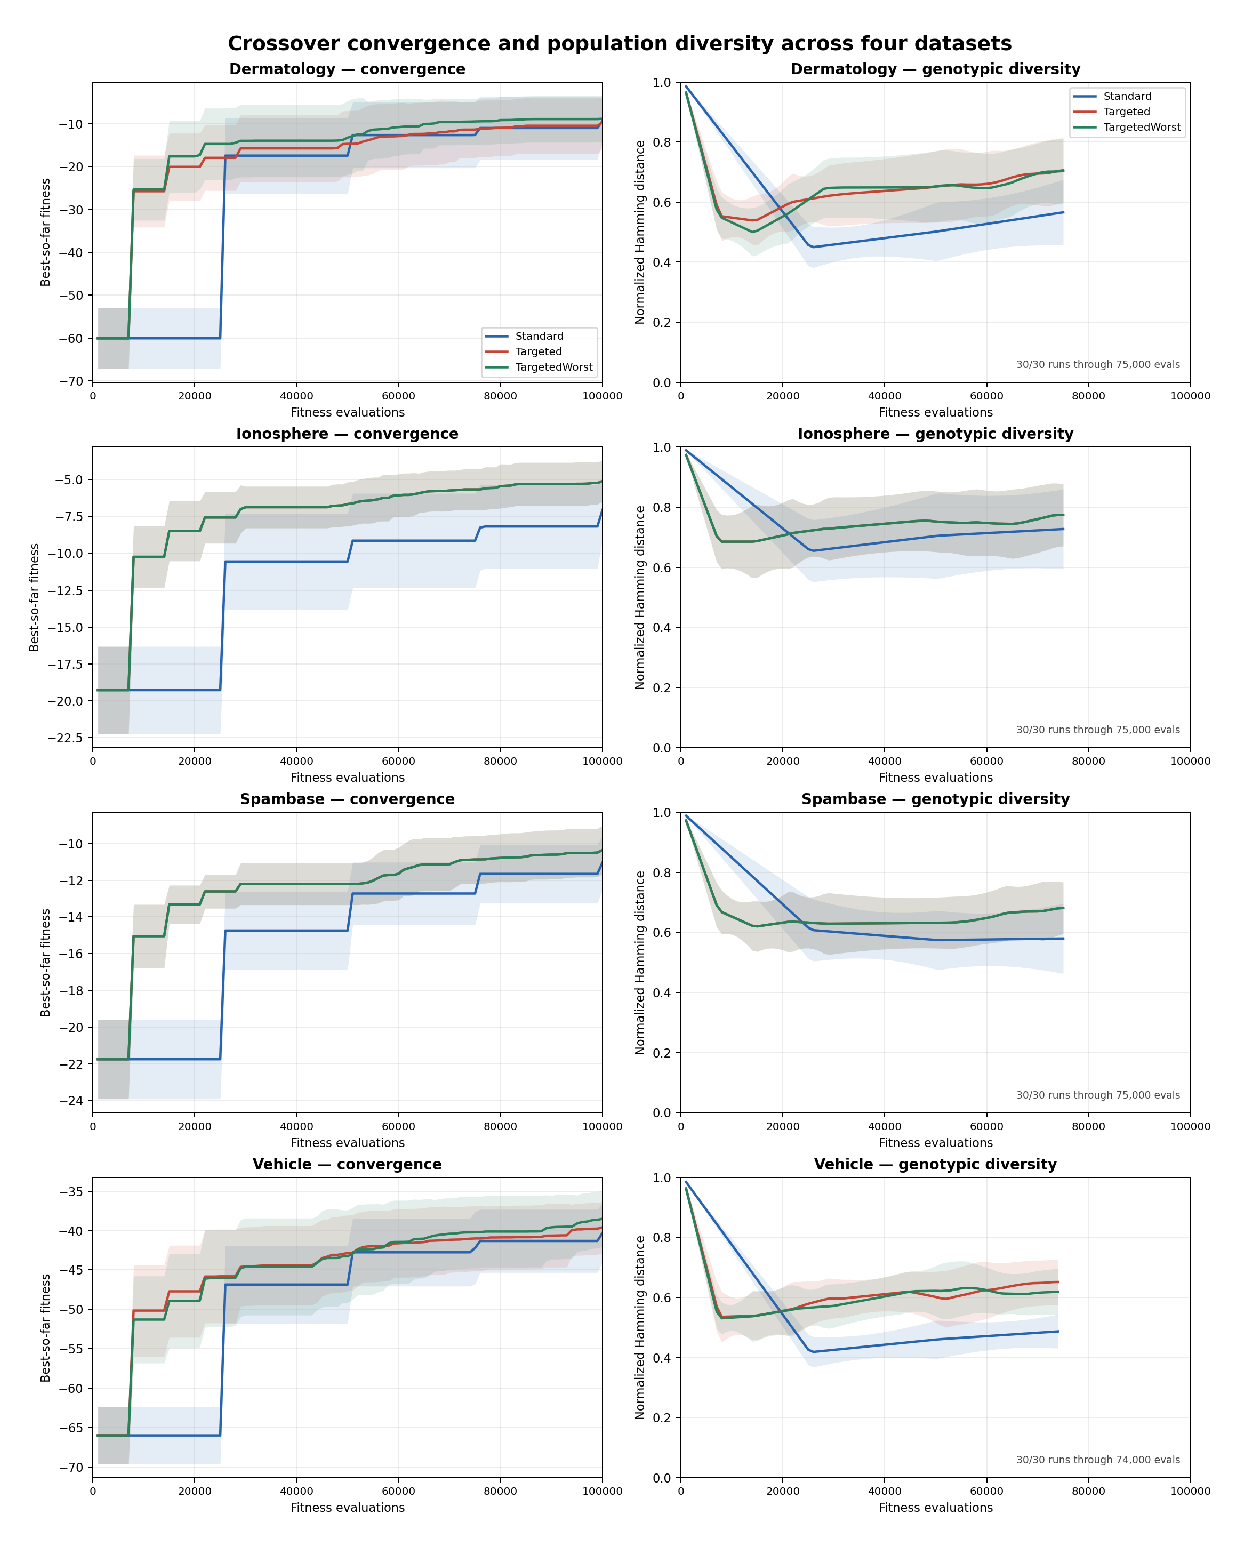
\includegraphics[width=\textwidth]{convergence_4datasets_8panels.pdf}
\caption{Convergence and population diversity of the Standard, Targeted, and TargetedWorst crossover operators on Dermatology, Ionosphere, Spambase, and Vehicle. The left column presents mean best-so-far fitness, while the right column presents mean normalized average pairwise Hamming distance. Results are aggregated over 30 independent runs per operator. Shaded regions represent the mean $\pm$ one standard deviation. Diversity curves are restricted to evaluation ranges with complete observations across all runs, whereas convergence curves extend to the fixed budget of 100,000 fitness evaluations.}
\label{fig:convergence_diversity}
\end{figure}

\subsection{Interpretability and Program Complexity}

Interpretability was evaluated through the complexity of the final,
expressed classification programs. Four complementary measures were
considered:
\begin{enumerate}
\item Program length in lexical tokens.
\item The number of distinct input features referenced.
\item The number of relational comparisons .
\item The number of conditional statements. 
\end{enumerate}
These measures characterize different aspects of the readability of
the generated rule systems: a program may be syntactically long without
introducing additional decision branches or input features.We analyzed
the final logged programs of the Standard, Targeted, and TargetedWorst
crossover variants on ten datasets. For each dataset-{}-operator combination,
up to 30 independently seeded runs were available. In total, 898 programs
were successfully extracted: 298 for Standard and 300 for each of
Targeted and TargetedWorst. The Standard results include 29 runs forDermatology
and 29 for Yeast; the remaining combinations contain 30 runs. The
measurements describe the final logged best programs, not the mean
complexity of the evolving populations.


\begin{table*}[t]
\centering
\caption{Complexity of final evolved programs. Values are mean $\pm$
standard deviation across independent runs. Program length is measured in
lexical tokens; $F$ is the number of distinct features, $C$ the number of
relational comparisons, and $I$ the number of conditional statements.}
\label{tab:rule_complexity}
\scriptsize
\resizebox{\textwidth}{!}{%
\begin{tabular}{llrrrrr}
\toprule
Dataset & Method & $n$ & Tokens & $F$ & $C$ & $I$ \\
\midrule
Dermatology & Standard & 29 & 105.76 $\pm$ 18.32 & 12.79 $\pm$ 3.02 & 8.45 $\pm$ 1.97 & 5.00 \\
Dermatology & Targeted & 30 & 94.47 $\pm$ 17.88 & 11.83 $\pm$ 2.29 & 7.77 $\pm$ 1.65 & 5.00 \\
Dermatology & TargetedWorst & 30 & 96.43 $\pm$ 18.44 & 12.30 $\pm$ 2.09 & 7.73 $\pm$ 1.55 & 5.00 \\
\midrule
Hepatitis & Standard & 30 & 56.03 $\pm$ 28.71 & 7.33 $\pm$ 2.68 & 3.80 $\pm$ 1.83 & 1.00 \\
Hepatitis & Targeted & 30 & 55.90 $\pm$ 30.52 & 7.87 $\pm$ 2.42 & 4.17 $\pm$ 1.84 & 1.00 \\
Hepatitis & TargetedWorst & 30 & 55.90 $\pm$ 30.52 & 7.87 $\pm$ 2.42 & 4.17 $\pm$ 1.84 & 1.00 \\
\midrule
Housevotes & Standard & 30 & 44.57 $\pm$ 23.25 & 4.50 $\pm$ 2.69 & 2.63 $\pm$ 1.65 & 1.00 \\
Housevotes & Targeted & 30 & 35.57 $\pm$ 13.52 & 4.80 $\pm$ 2.01 & 2.60 $\pm$ 1.59 & 1.00 \\
Housevotes & TargetedWorst & 30 & 35.57 $\pm$ 13.52 & 4.80 $\pm$ 2.01 & 2.60 $\pm$ 1.59 & 1.00 \\
\midrule
Ionosphere & Standard & 30 & 54.67 $\pm$ 28.10 & 6.60 $\pm$ 3.04 & 3.60 $\pm$ 2.04 & 1.00 \\
Ionosphere & Targeted & 30 & 51.90 $\pm$ 17.00 & 6.43 $\pm$ 2.06 & 3.70 $\pm$ 1.42 & 1.00 \\
Ionosphere & TargetedWorst & 30 & 51.90 $\pm$ 17.00 & 6.43 $\pm$ 2.06 & 3.70 $\pm$ 1.42 & 1.00 \\
\midrule
Optdigits & Standard & 30 & 162.23 $\pm$ 18.19 & 20.93 $\pm$ 3.38 & 13.13 $\pm$ 1.91 & 9.00 \\
Optdigits & Targeted & 30 & 147.13 $\pm$ 12.33 & 18.90 $\pm$ 2.68 & 12.03 $\pm$ 1.59 & 9.00 \\
Optdigits & TargetedWorst & 30 & 144.37 $\pm$ 16.25 & 19.30 $\pm$ 2.69 & 12.13 $\pm$ 1.43 & 9.00 \\
\midrule
Segment & Standard & 30 & 132.57 $\pm$ 19.12 & 12.00 $\pm$ 1.78 & 9.40 $\pm$ 1.89 & 6.00 \\
Segment & Targeted & 30 & 117.73 $\pm$ 13.16 & 10.87 $\pm$ 1.46 & 8.70 $\pm$ 1.47 & 6.00 \\
Segment & TargetedWorst & 30 & 119.27 $\pm$ 12.27 & 11.53 $\pm$ 2.05 & 8.90 $\pm$ 1.49 & 6.00 \\
\midrule
Spambase & Standard & 30 & 72.30 $\pm$ 33.92 & 10.33 $\pm$ 3.92 & 6.00 $\pm$ 2.82 & 1.00 \\
Spambase & Targeted & 30 & 72.77 $\pm$ 28.17 & 11.17 $\pm$ 3.28 & 6.87 $\pm$ 2.56 & 1.00 \\
Spambase & TargetedWorst & 30 & 72.77 $\pm$ 28.17 & 11.17 $\pm$ 3.28 & 6.87 $\pm$ 2.56 & 1.00 \\
\midrule
Thyroid & Standard & 30 & 79.27 $\pm$ 26.96 & 7.67 $\pm$ 2.51 & 4.63 $\pm$ 1.83 & 2.00 \\
Thyroid & Targeted & 30 & 70.10 $\pm$ 22.42 & 7.60 $\pm$ 2.57 & 5.00 $\pm$ 2.00 & 2.00 \\
Thyroid & TargetedWorst & 30 & 75.67 $\pm$ 23.03 & 8.33 $\pm$ 1.75 & 5.47 $\pm$ 1.53 & 2.00 \\
\midrule
Vehicle & Standard & 30 & 115.63 $\pm$ 24.02 & 10.77 $\pm$ 2.61 & 6.87 $\pm$ 2.71 & 3.00 \\
Vehicle & Targeted & 30 & 94.93 $\pm$ 22.02 & 9.90 $\pm$ 2.50 & 5.60 $\pm$ 2.18 & 3.00 \\
Vehicle & TargetedWorst & 30 & 91.03 $\pm$ 17.33 & 9.87 $\pm$ 1.91 & 5.60 $\pm$ 1.96 & 3.00 \\
\midrule
Yeast & Standard & 29 & 159.24 $\pm$ 14.86 & 7.83 $\pm$ 0.47 & 11.38 $\pm$ 1.86 & 9.00 \\
Yeast & Targeted & 30 & 156.80 $\pm$ 14.26 & 7.67 $\pm$ 0.48 & 10.87 $\pm$ 1.59 & 9.00 \\
Yeast & TargetedWorst & 30 & 154.47 $\pm$ 14.30 & 7.87 $\pm$ 0.35 & 10.73 $\pm$ 1.17 & 9.00 \\
\bottomrule
\end{tabular}}
\end{table*}

To assess paired differences in final program length, runs were matched
by dataset and random seed and compared using the Wilcoxon signed-rank
test. The Holm procedure was applied to the family of 20 length comparisons
(Standard versus Targeted and Standard versus TargetedWorst for each
of the ten datasets). After correction, Standard generated significantly
longer programs on Optdigits, Segment, and Vehicle relative to both
alternatives (Table \ref{tab:complexity_tests}). No comparison of
the number of distinct features or relational comparisons remained
significant after the corresponding Holm corrections. The number of
conditional statements was identical across the three variants within
each dataset in these extracted results. Thus, longer expressions
did not necessarily entail more decision branches.

\begin{table}[t]
\centering
\caption{Holm-adjusted Wilcoxon $p$-values for the significant
paired comparisons of final program length. The positive mean differences
indicate longer Standard programs.}
\label{tab:complexity_tests}
\small
\begin{tabular}{llrr}
\toprule
Dataset & Comparison & Mean difference & Adjusted $p$ \\
\midrule
Optdigits & Standard--Targeted & 15.10 & 0.03490 \\
Optdigits & Standard--TargetedWorst & 17.87 & 0.00654 \\
Segment & Standard--Targeted & 14.83 & 0.01714 \\
Segment & Standard--TargetedWorst & 13.30 & 0.01163 \\
Vehicle & Standard--Targeted & 20.70 & 0.00987 \\
Vehicle & Standard--TargetedWorst & 24.60 & 0.00462 \\
\bottomrule
\end{tabular}
\end{table}

\paragraph{Examples of evolved rules.} 

The following examples are taken verbatim from the final logged programsfor
the Ionosphere dataset (seed 1). Both runs used a strict budget of
100,000 fitness evaluations. Standard reached a training classification
error of 8.23\textbackslash\% and a test error of 17.14\%, whereas
Targeted reached 5.06\% and 11.43\%, respectively. The TargetedWorst
program was identical to the Targeted program for this seed. These
examples illustrate the form and complexity of the learned expressions,
but should not be interpreted as a representative performance comparison
from a single seed.

\noindent\textbf{Standard:}
\begin{lstlisting}[basicstyle=\ttfamily\scriptsize,breaklines=true]
if(!(x1<=cos((sin(x33)*x17))&x18>((-8.55)+(-1.2))|x2*x23>=x7&x9>x24|x5<sin(x20)&!(x19<cos(((x3*(x27*sin(x29)))-(-9.40)))))) CLASS=0.00
else 
CLASS=1.00
\end{lstlisting}

\noindent\textbf{Targeted (also TargetedWorst):}
\begin{lstlisting}[basicstyle=\ttfamily\scriptsize,breaklines=true]
if(!(x1<=cos((sin(x33)*x9))|!(!(x5<=(x21*x16)|!(x16>=sin((-89.27))&!(x29<=cos((-9.0)))))))) CLASS=0.00
else 
CLASS=1.00
\end{lstlisting}

\paragraph{Program growth and bloat.}

Additional illustrative evolutionary traces were examined for the
original GenClass baseline and Standard on Shuttle and Pirvision over
2,000 generations. In these individual runs, Standard yielded longer
final programs, but program length fluctuated and sometimes decreased
during optimization rather than increasing monotonically. Importantly,
these traces are not controlled equal-evaluation comparisons: Standard
used 6,335,527 versus 1,783,945 fitness evaluations on Shuttle and
6,776,246 versus 2,072,441 on Pirvision. Moreover, the recorded lengths
refer to reported best programs, not population-wide mean genome or
phenotype sizes. Accordingly, the evidence supports the narrower finding
that some greedy crossover variants increase final expressed rule
length; it does not establish the presence or absence of population-level
genetic programming bloat. A definitive bloat study would require
matched fitness-evaluation budgets, multiple independent baseline
runs, and population-level complexity measurements throughout evolution.

\subsection{Influence of Dataset Characteristics on Classification Performance}

To investigate whether the benefit of the proposed crossover mechanism
depends on dataset characteristics, we examined all 31 datasets listed
in Table \ref{tab:The-main-characteristics}. For each dataset, the
improvement was defined as $\Delta E=E_{\mathrm{CLASS}}-E_{\mathrm{STANDARD}}$,
where $E$ denotes the mean test classification error (in percentage
points) reported in Table \ref{tab:methods_comparison}. Thus, positive
values indicate lower error for STANDARD. Spearman's rank correlation
was used to assess associations between $\Delta E$ and the numbers
of patterns, input features, and classes. Each dataset constituted
one observation ($N=31$); repeated runs were not treated as independent
dataset-level observations.

The association between improvement and dataset size was weak ($\rho=-0.087$,
$p=0.643$), as was the association with the number of features ($\rho=0.071$,
$p=0.706$). The number of classes showed a positive association ($\rho=0.395$,
nominal $p=0.0277$), suggesting that larger improvements may occur
in problems with more classes. However, this association did not remain
statistically significant after Holm correction across the three correlations.
The result should therefore be considered exploratory rather than
evidence of a robust dependence on class count.

We also separated the datasets into binary ($N=9$) and multiclass
($N=22$) problems. STANDARD reduced the mean classification error
relative to CLASS on 8 of the 9 binary datasets and 20 of the 22 multiclass
datasets. The average improvements were 1.72 and 3.12 percentage points,
respectively. Nevertheless, a two-sided Mann-{}-Whitney U test did
not identify a statistically significant difference in dataset-level
improvements between these groups ($p=0.267$).

The previously mentioned results do not reveal a clear monotonic relationship
between the advantage of STANDARD and the number of patterns or features.
Although the class-count analysis suggests a potentially interesting
trend, the available dataset-level evidence is insufficient to establish
that the proposed crossover mechanism systematically benefits more
from a larger number of classes. Moreover, these observational comparisons
do not isolate dataset size or class count from other differences
in problem difficulty and structure.

\subsection{Analysis of Accepted Crossover Improvements}

To quantify the behavior of the six crossover variants, we recorded
the number of accepted crossover improvements at each generation in
30 independent runs on the Dermatology dataset. All runs used the
same limit of 100,000 fitness evaluations. An accepted improvement
denotes an improvement accepted by the crossover mechanism; it does
not necessarily indicate a new global-best individual. Table \ref{tab:accepted-crossover-improvements}
reports the mean and sample standard deviation across runs. The per-generation
measure was computed for each run by dividing its total number of
accepted improvements by its number of completed generations, before
aggregating across runs.

\begin{table}[t]
\centering
\caption{Accepted crossover improvements on the Dermatology dataset
(mean $\pm$ sample standard deviation over 30 independent runs).
The last column normalizes by the number of crossover evaluations,
not by the total fitness-evaluation budget.}
\label{tab:accepted-crossover-improvements}
\small
\setlength{\tabcolsep}{4pt}
\begin{tabular}{lrrr}
\toprule
Crossover variant & Accepted/run & Accepted/generation & Accepted/1,000 cross. evals \\
\midrule
Standard        & $968.40\pm192.93$ & $24.46\pm4.76$ & $12.26\pm2.41$ \\
Standard+Elite  & $817.57\pm196.46$ & $20.62\pm4.78$ & $10.34\pm2.43$ \\
Standard+Block  & $887.27\pm144.49$ & $22.47\pm3.55$ & $11.24\pm1.80$ \\
Targeted        & $555.90\pm85.48$  & $5.62\pm0.86$  & $27.19\pm4.30$ \\
Targeted+Full   & $558.37\pm75.82$  & $5.63\pm0.77$  & $27.23\pm3.90$ \\
TargetedWorst   & $294.40\pm84.40$  & $2.97\pm0.85$  & $15.19\pm4.23$ \\
\bottomrule
\end{tabular}
\end{table}

Standard produced the largest number of accepted improvements per
generation($24.46\pm4.76$), followed by Standard+Block ($22.47\pm3.55$)
and Standard+Elite ($20.62\pm4.78$). The targeted variants produced
fewer accepted improvements per generation, partly because they performed
fewer crossover evaluations within each generation. Accordingly, we
also report accepted improvements per 1,000 crossover evaluations.
By this measure, Targeted and Targeted+Full achieved approximately
27.2 accepted improvements, compared with 12.3 for Standard. This
difference concerns acceptance frequency, not necessarily the magnitude
of improvement or final classification accuracy.

To examine how acceptance evolves during the search, we divided the
common 100,000-fitness-evaluation budget into ten intervals. For each
run, the accepted improvements and crossover evaluations of a generation
were assigned to the interval containing that generation's ending
cumulative fitness- evaluation count. Figure \ref{fig:accepted-crossover-count}
shows the resulting mean counts. The Standard variants generally exhibit
a reduction in the number of accepted improvements from the early
to the later intervals. The targeted variants exhibit more irregular
bin counts.

\begin{figure}[t]
\centering
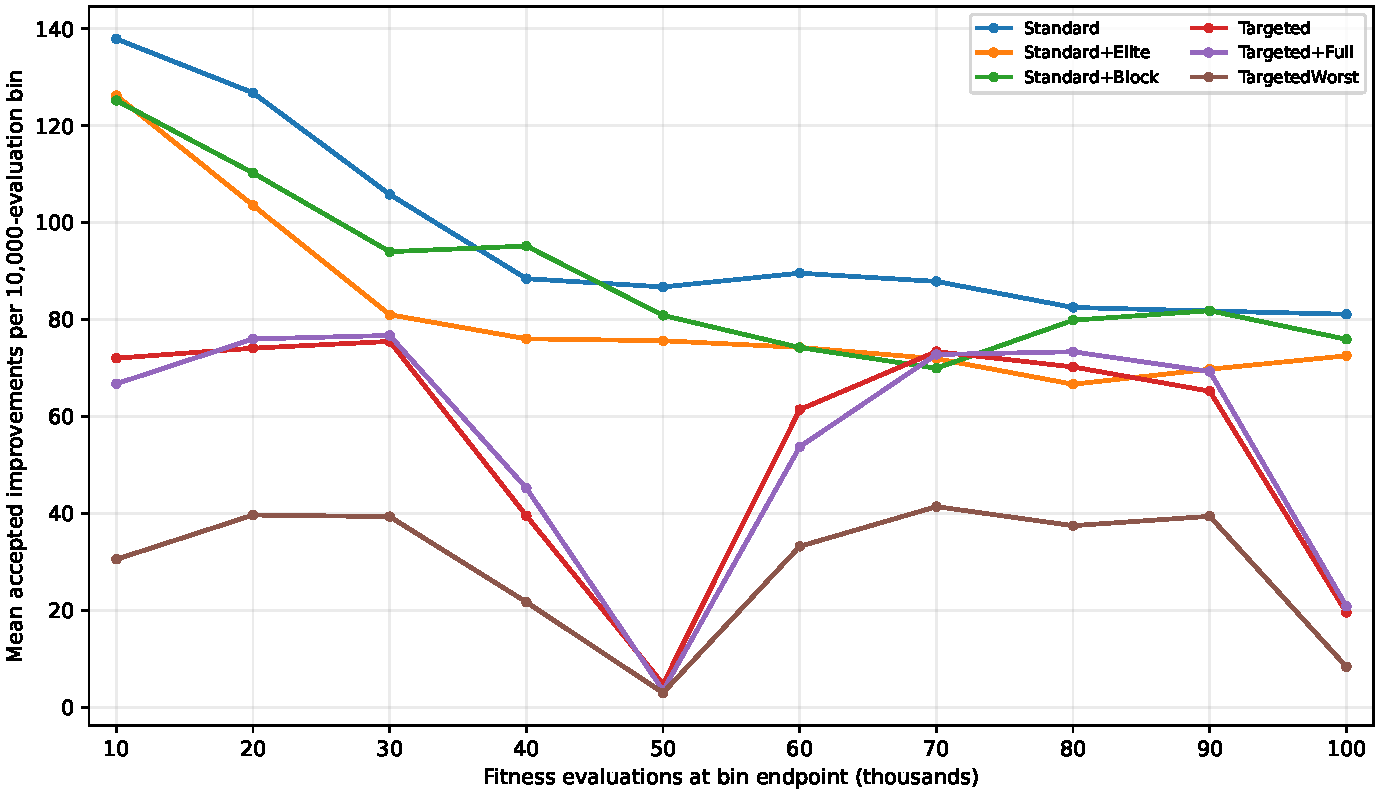
\includegraphics[width=\linewidth]{accepted_improvements_by_budget.pdf}
\caption{Mean number of accepted crossover improvements in successive
10,000-fitness-evaluation intervals on Dermatology (30 runs per variant).
Whole generations are assigned to the interval in which they finish; therefore,
short-term fluctuations may reflect bin boundaries rather than changes in
search behavior.}
\label{fig:accepted-crossover-count}
\end{figure}

Figure \ref{fig:accepted-crossover-rate} accounts for the different
numbers of crossover evaluations in each interval. The Standard acceptance
frequency falls from approximately 17.3 to 10.4 accepted improvements
per 1,000 crossover evaluations between the first and last intervals.
In contrast, Targeted and Targeted+Full remain at approximately 25-{}-29
accepted improvements per 1,000 crossover evaluations across most
intervals. Thus, although the targeted variants accept fewer improvements
per generation, they exhibit a higher acceptance frequency per crossover
evaluation.

\begin{figure}[t]
\centering
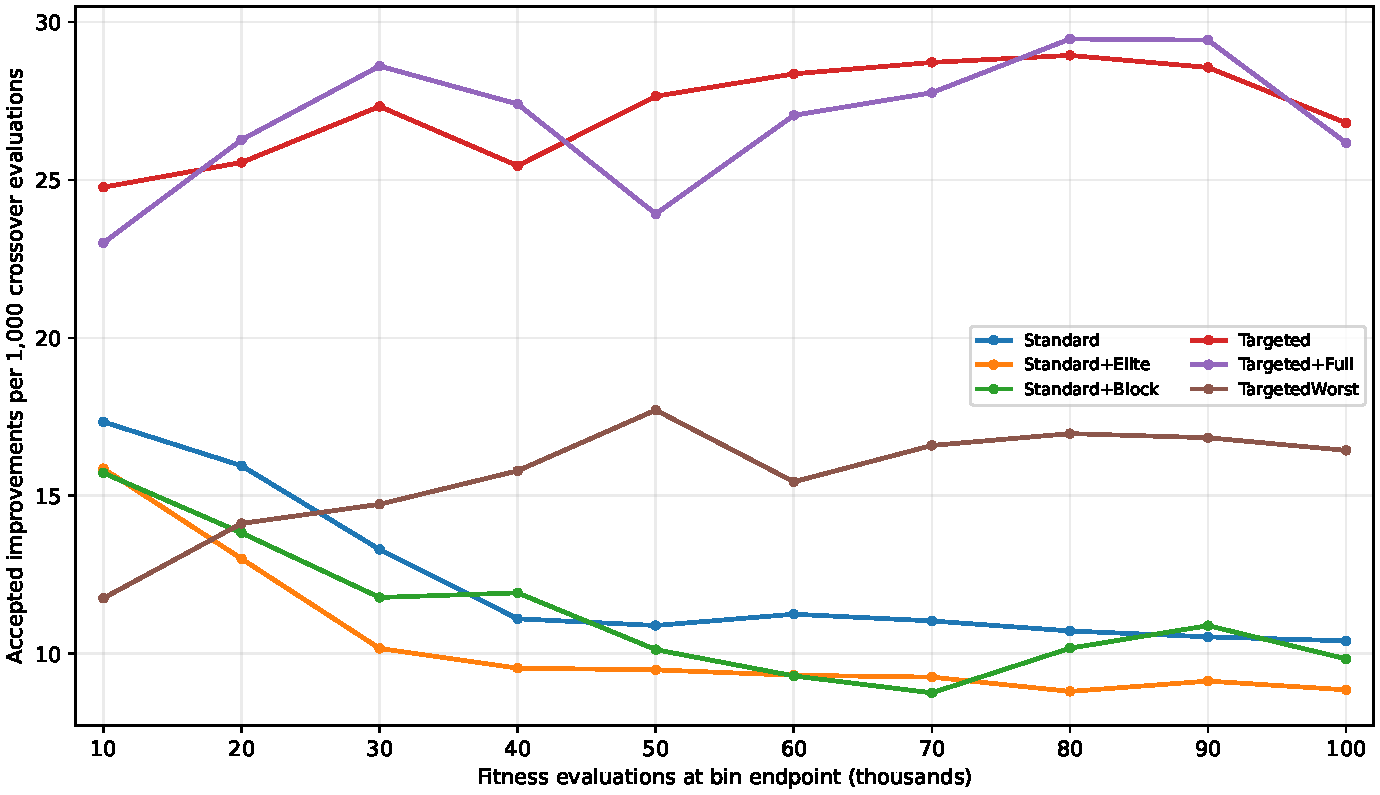
\includegraphics[width=\linewidth]{acceptance_rate_by_budget.pdf}
\caption{Accepted crossover improvements per 1,000 crossover evaluations
across the fitness-evaluation budget. Each point is the ratio of the mean
accepted improvements to the mean crossover evaluations within the corresponding
interval (30 runs per variant). The binning uses generation endpoints.}
\label{fig:accepted-crossover-rate}
\end{figure}

These findings describe the acceptance dynamics on Dermatology and
should not be interpreted as evidence of superiority across all datasets.
In particular, acceptance frequency alone does not establish whether
a method yields better final classification performance.

\section{Conclusions\label{sec:Conclusions}}

This work introduced an additional crossover procedure into the GenClass
method. At each generation, after the conventional genetic operators
have been applied, $N_{K}$ randomly selected chromosomes undergo
$k$ crossover trials. A candidate chromosome replaces the current
chromosome only when it achieves a strictly lower training classification
error. Three variants, denoted Standard, Targeted, and TargetedWorst,
were evaluated on 31 classification datasets. Standard applies one-point
crossover using donors selected from the population. It reduced the
average classification error of the original method from 16.13\% to
13.42\%, corresponding to a relative reduction of approximately 16.8\%,
and obtained the lowest error on 19 of the 31 datasets among the eleven
compared methods. Its average error was also lower than those of the
additional reference classifiers, including CART (19.42\%) and SVM
(21.97\%). The improvement over the original method remained statistically
significant in the sensitivity analysis that excluded four related
EEG-derived datasets and applied Holm correction for multiple comparisons.

The comparison of the three variants revealed that additional grammatical
and class-specific guidance did not necessarily improve classification
performance. Targeted and TargetedWorst select donor chromosomes from
an elite fraction of the population and exchange bounded blocks of
codons at semantically compatible positions. TargetedWorst further
restricts the modified region according to the worst-performing class.
Nevertheless, Standard achieved a lower average classification error
than both targeted variants. The respective mean errors were 13.42\%
for Standard, 15.08\% for Targeted, and 15.42\% for TargetedWorst,
compared with 16.13\% for the original GenClass method. In the reported
pairwise comparisons, Standard outperformed both targeted variants,
whereas no statistically significant difference was established between
Targeted and TargetedWorst. Comparisons against the original method
indicated that Standard provided the most robust improvement under
the more conservative sensitivity analysis; the evidence supporting
the targeted variants was less conclusive.

A possible explanation for these findings concerns the different recombination
mechanisms. Standard selects donors from the entire population and
exchanges chromosome segments following randomly selected crossover
points, whereas the targeted variants select donors from the best
20\% of the population and transfer blocks of at most $B_{\max}$
codons. The additional convergence and population diversity experiments
described in subsection \ref{subsec:Convergence-and-Population},
conducted on Dermatology, Ionosphere, Spambase, and Vehicle, showed
that the targeted variants often maintained greater genotypic diversity
than Standard, as measured by normalized average pairwise Hamming
distance. However, this higher diversity did not consistently translate
into better final fitness or lower classification error. Thus, the
lower average classification error achieved by Standard in the present
experiments cannot be explained simply by greater preservation of
genotypic diversity. Donor selection, the extent of exchanged genetic
material, and the balance between exploration and exploitation are
plausible contributing factors, but the present results do not establish
a causal relationship between these mechanisms and generalization
performance. Donor selection, the extent of exchanged genetic material,
and the balance between exploration and exploitation are plausible
contributing factors, but the present results do not establish a causal
relationship between these mechanisms and generalization performance.

The convergence experiments also clarified an implementation-specific
property of the targeted operators on binary classification problems.
When the number of classes is two, the single explicitly encoded rule
occupies the entire chromosome; consequently, the class-based restriction
of TargetedWorst does not narrow the set of eligible crossover positions
relative to Targeted. This explains the identical trajectories observed
for these operators on the binary datasets considered in the convergence
analysis. Their behavior can differ on multiclass problems, where
the chromosome contains separate rule-encoding segments.

The number of chromosomes subjected to additional crossover also influenced
performance, particularly at its smallest tested value. The setting
$N_{K}=2$ performed significantly worse than the larger settings,
whereas differences among $N_{K}=5$, $10$, and $15$ were small
and not statistically significant. Although $N_{K}=15$ yielded the
lowest average error and the best mean rank, its advantage over the
other moderate settings was not statistically established. Therefore,
a moderate number of selected chromosomes appears sufficient under
the examined experimental configuration.

Several limitations should be acknowledged. The additional procedure
requires up to $N_{K}k$ candidate fitness evaluations per generation,
corresponding to 200 evaluations for the parameter configuration used
in the experiments, while the conventional genetic operators generate
$p_{s}N_{c}=450$ offspring per generation. The parameters $k$, $\rho$,
and $B_{\max}$ were kept fixed, and their individual effects were
not systematically examined. The conclusions are therefore restricted
to the evaluated datasets, parameter settings, and classification
tasks. Moreover, four EEG-derived benchmark problems originate from
related recordings and cannot be treated as fully independent observations.
Although a sensitivity analysis excluding these problems was performed,
the remaining datasets do not necessarily represent a random sample
of all classification tasks.

It should also be emphasized that the objective of this study is to
assess the effects of additional crossover strategies within the GenClass
framework, rather than to establish GenClass as a universally superior
classification method. The comparisons with other classifiers provide
supplementary performance references and should not be interpreted
as a comprehensive benchmark of supervised learning algorithms. Different
classification methods may be more suitable for different datasets
and application domains.

An additional limitation concerns the availability of run-level observations.
For the main cross-validation experiments, the individual results
of the 30 independent runs per fold were not retained, preventing
the estimation of run-to-run standard deviations and within-dataset
statistical tests from those experiments. In contrast, run-level observations
were retained for the supplementary convergence and population diversity
experiments reported in subsection \ref{subsec:Convergence-and-Population}.
Accordingly, small differences in average classification error should
be interpreted cautiously. Furthermore, because the greedy acceptance
criterion uses training classification error, the additional refinement
may increase the risk of overfitting, particularly on small datasets
such as Hepatitis and Appendicitis. The present diversity measurements
describe genotypic variation and do not, by themselves, demonstrate
improved generalization.

Future research should extend the convergence and population diversity
analysis to more datasets and investigate the effects of the elite
fraction $\rho$, maximum block size $B_{\max}$, and alternative
donor-selection policies. Hybrid operators combining random and grammatically
guided exchanges could also be examined. In addition, the number of
selected chromosomes $N_{K}$ and the number of crossover trials $k$
could be adapted dynamically during evolution; values of $N_{K}$
greater than 15 merit investigation because the largest tested setting
achieved the best mean rank without a statistically significant advantage.
Further studies should retain run-level results across the full cross-validation
protocol, assess generalization and overfitting more directly, and
report computational cost alongside predictive performance. Finally,
parallel implementations and applications to larger datasets, regression
tasks, and other Grammatical Evolution methods would help establish
the broader applicability of the proposed crossover procedure.

\vspace{6pt}


\authorcontributions{G.G. and I.G.T. conducted the experiments, employing several datasets
and provided the comparative experiments. V.C. performed the statistical
analysis and prepared the manuscript. All authors have read and agreed
to the published version of the manuscript.}

\funding{This research has been financed by the European Union : Next Generation
EU through the Program Greece 2.0 National Recovery and Resilience
Plan , under the call RESEARCH -- CREATE -- INNOVATE, project name
“iCREW: Intelligent small craft simulator for advanced crew training
using Virtual Reality techniques\textquotedbl{} (project code:TAEDK-06195).}

\institutionalreview{Not applicable.}

\informedconsent{Not applicable.}

\dataavailability{The original contributions presented in this study are included in
the article. Further inquiries can be directed to the corresponding
author. }

\conflictsofinterest{The authors declare no conflicts of interest.}

\begin{adjustwidth}{-\extralength}{0cm}{}

\reftitle{References}
\begin{thebibliography}{999}
\bibitem{holland}J.H. Holland, Genetic algorithms. Scientific american
\textbf{267}, pp. 66-73, 1992.

\bibitem{ec_review}N. Yusup, A. M. Zain, S. Z. M. Hashim, Evolutionary
techniques in optimizing machining parameters: Review and recent applications
(2007--2011), Expert Systems with Applications \textbf{39.10}, pp.
9909-9927, 2012.

\bibitem{gen1}J. Stender, Parallel Genetic Algorithms:Theory \& Applications.
Edition: IOS Press, 1993. 

\bibitem{gen2}D. Goldberg, Genetic Algorithms in Search, Optimization
and Machine Learning, Addison-Wesley Publishing Company, Reading,
Massachussets, 1989.

\bibitem{gen3}Z. Michaelewicz, Genetic Algorithms + Data Structures
= Evolution Programs. Springer - Verlag, Berlin, 1996.

\bibitem{ga_problem1}Y.H. Santana, R.M. Alonso, G.G. Nieto, L. Martens,
W. Joseph, D. Plets, Indoor genetic algorithm-based 5G network planning
using a machine learning model for path loss estimation, Appl. Sci.
\textbf{12}, 3923. 2022.

\bibitem{ga_problem2}X. Liu, D. Jiang, B. Tao, G. Jiang, Y. Sun,
J. Kong, B. Chen, Genetic algorithm-based trajectory optimization
for digital twin robots, Front. Bioeng. Biotechnol \textbf{9}, 793782,
2022.

\bibitem{ga_problem3}K. Nonoyama, Z.Liu, T. Fujiwara, M.M. Alam,
T. Nishi, Energy-efficient robot configuration and motion planning
using genetic algorithm and particle swarm optimization, Energies
\textbf{15}, 2074, 2022.

\bibitem{ga_problem4}K. Liu, B. Deng, Q. Shen, J. Yang, Y. Li, Optimization
based on genetic algorithms on energy conservation potential of a
high speed SI engine fueled with butanol--gasoline blends, Energy
Rep. \textbf{8}, pp. 69--80, 2022.

\bibitem{ga_problem5}G. Zhou, S. Zhu, S. Luo, Location optimization
of electric vehicle charging stations: Based on cost model and genetic
algorithm, Energy \textbf{247}, 123437, 2022.

\bibitem{Choudhury} Choudhury, S.; Rana, M.; Chakraborty, A.; Majumder,
S.; Roy, S.; RoyChowdhury, A.; Datta, S. Design of patient specific
basal dental implant using Finite Element method and Artificial Neural
Network technique. J. Eng. Med. 2022, 236, 1375--1387.

\bibitem{Chen} Chen, Q.; Hu, X. Design of intelligent control system
for agricultural greenhouses based on adaptive improved genetic algorithm
for multi-energy supply system. Energy Rep. 2022, 8, 12126--12138.

\bibitem{ge1}M. O’Neill, C. Ryan, Grammatical evolution, IEEE Trans.
Evol. Comput. \textbf{5,}pp. 349--358, 2001.

\bibitem{bnf1}J. W. Backus. The Syntax and Semantics of the Proposed
International Algebraic Language of the Zurich ACM-GAMM Conference.
Proceedings of the International Conference on Information Processing,
UNESCO, 1959, pp.125-132.

\bibitem{ge_program1}C. Ryan, J. Collins, M. O’Neill, Grammatical
evolution: Evolving programs for an arbitrary language. In: Banzhaf,
W., Poli, R., Schoenauer, M., Fogarty, T.C. (eds) Genetic Programming.
EuroGP 1998. Lecture Notes in Computer Science, vol 1391. Springer,
Berlin, Heidelberg, 1998.

\bibitem{ge_program2}M. O’Neill, M., C. Ryan, Evolving Multi-line
Compilable C Programs. In: Poli, R., Nordin, P., Langdon, W.B., Fogarty,
T.C. (eds) Genetic Programming. EuroGP 1999. Lecture Notes in Computer
Science, vol 1598. Springer, Berlin, Heidelberg, 1999.

\bibitem{ge_credit}A. Brabazon, M. O'Neill, Credit classification
using grammatical evolution, Informatica \textbf{30.3}, 2006.

\bibitem{ge_intrusion}S. Şen, J.A. Clark. A grammatical evolution
approach to intrusion detection on mobile ad hoc networks, In: Proceedings
of the second ACM conference on Wireless network security, 2009.

\bibitem{ge_de}I.G. Tsoulos, I.E. Lagaris, Solving differential equations
with genetic programming, Genet Program Evolvable Mach \textbf{7},
pp. 33--54, 2006.

\bibitem{ge_water}L. Chen, C.H. Tan, S.J. Kao, T.S. Wang, Improvement
of remote monitoring on water quality in a subtropical reservoir by
incorporating grammatical evolution with parallel genetic algorithms
into satellite imagery, Water Research \textbf{ 42}, pp. 296-306,
2008.

\bibitem{ge_ant}J. Tavares, F.B. Pereira, Automatic Design of Ant
Algorithms with Grammatical Evolution. In: Moraglio, A., Silva, S.,
Krawiec, K., Machado, P., Cotta, C. (eds) Genetic Programming. EuroGP
2012. Lecture Notes in Computer Science, vol 7244. Springer, Berlin,
Heidelberg, 2012.

\bibitem{ge_trig}C. Ryan, M. O’Neill, J.J. Collins, Grammatical evolution:
Solving trigonometric identities, proceedings of Mendel. Vol. 98.
1998.

\bibitem{ge_music}A.O. Puente, R. S. Alfonso, M. A. Moreno, Automatic
composition of music by means of grammatical evolution, In: APL '02:
Proceedings of the 2002 conference on APL: array processing languages:
lore, problems, and applications July 2002 Pages 148--155. 

\bibitem{ge_nn}Lídio Mauro Limade Campo, R. Célio Limã Oliveira,Mauro
Roisenberg, Optimization of neural networks through grammatical evolution
and a genetic algorithm, Expert Systems with Applications \textbf{56},
pp. 368-384, 2016.

\bibitem{ge_nn2}K. Soltanian, A. Ebnenasir, M. Afsharchi, Modular
Grammatical Evolution for the Generation of Artificial Neural Networks,
Evolutionary Computation \textbf{30}, pp 291--327, 2022.

\bibitem{ge_pacman}E. Galván-López, J.M. Swafford, M. O’Neill, A.
Brabazon, Evolving a Ms. PacMan Controller Using Grammatical Evolution.
In: , et al. Applications of Evolutionary Computation. EvoApplications
2010. Lecture Notes in Computer Science, vol 6024. Springer, Berlin,
Heidelberg, 2010.

\bibitem{ge_supermario}N. Shaker, M. Nicolau, G. N. Yannakakis, J.
Togelius, M. O'Neill, Evolving levels for Super Mario Bros using grammatical
evolution, 2012 IEEE Conference on Computational Intelligence and
Games (CIG), 2012, pp. 304-31.

\bibitem{ge_energy}D. Martínez-Rodríguez, J. M. Colmenar, J. I. Hidalgo,
R.J. Villanueva Micó, S. Salcedo-Sanz, Particle swarm grammatical
evolution for energy demand estimation, Energy Science and Engineering
\textbf{8}, pp. 1068-1079, 2020.

\bibitem{ge_comb}N. R. Sabar, M. Ayob, G. Kendall, R. Qu, Grammatical
Evolution Hyper-Heuristic for Combinatorial Optimization Problems,
IEEE Transactions on Evolutionary Computation \textbf{17}, pp. 840-861,
2013.

\bibitem{ge_crypt}C. Ryan, M. Kshirsagar, G. Vaidya, G. et al. Design
of a cryptographically secure pseudo random number generator with
grammatical evolution. Sci Rep \textbf{12}, 8602, 2022.

\bibitem{ge_decision}P.J. Pereira, P. Cortez, R. Mendes, Multi-objective
Grammatical Evolution of Decision Trees for Mobile Marketing user
conversion prediction, Expert Systems with Applications \textbf{168},
114287, 2021.

\bibitem{ge_analog}F. Castejón, E.J. Carmona, Automatic design of
analog electronic circuits using grammatical evolution, Applied Soft
Computing \textbf{62}, pp. 1003-1018, 2018.

\bibitem{ge_wikipedia}L. Araujo, J. Martinez-Romo, A. Duque, Discovering
taxonomies in Wikipedia by means of grammatical evolution. Soft Comput
\textbf{22}, pp. 2907--2919, 2018. 

\bibitem{ge_trading}C. Martín, D. Quintana, P. Isasi, Grammatical
Evolution-based ensembles for algorithmic trading, Applied Soft Computing
\textbf{84}, 105713, 2019.

\bibitem{ge_bio}Moore, J.H., Sipper, M. (2018). Grammatical Evolution
Strategies for Bioinformatics and Systems Genomics. In: Ryan, C.,
O'Neill, M., Collins, J. (eds) Handbook of Grammatical Evolution.
Springer, Cham. https://doi.org/10.1007/978-3-319-78717-6\_16

\bibitem{ge_glykemia}Hidalgo, J. I., Colmenar, J. M., Risco-Martin,
J. L., Cuesta-Infante, A., Maqueda, E., Botella, M., \& Rubio, J.
A. (2014). Modeling glycemia in humans by means of grammatical evolution.
Applied Soft Computing, 20, 40-53.

\bibitem[(2020)]{genclassMain}Tsoulos, I. G. (2020). Creating classification
rules using grammatical evolution. International Journal of Computational
Intelligence Studies, 9(1-2), 161-171.

\bibitem[(2020)]{genclassSoftx}Anastasopoulos, N.; Tsoulos, I.G.;
Tzallas, A. GenClass: A parallel tool for data classification based
on Grammatical Evolution. SoftwareX 2021, 16, 100830.

\bibitem{genclassPollution}Spyrou, E. D., Stylios, C., \& Tsoulos,
I. (2023). Classification of CO Environmental Parameter for Air Pollution
Monitoring with Grammatical Evolution. Algorithms, 16(6), 300.

\bibitem[(2023)]{genClassNetwork}Margariti, S. V., Tsoulos, I. G.,
Kiousi, E., \& Stergiou, E. (2024). Traffic Classification in Software-Defined
Networking Using Genetic Programming Tools. Future Internet, 16(9),
338.

\bibitem[(1989)]{uci} M. Kelly, R. Longjohn, K. Nottingham, The UCI
Machine Learning Repository, \url{https://archive.ics.uci.edu}.

\bibitem{Keel}J. Alcalá-Fdez, A. Fernandez, J. Luengo, J. Derrac,
S. García, L. Sánchez, F. Herrera. KEEL Data-Mining Software Tool:
Data Set Repository, Integration of Algorithms and Experimental Analysis
Framework. Journal of Multiple-Valued Logic and Soft Computing 17,
pp. 255-287, 2011.

\bibitem[Tzimourta(2018)]{alcohol}Tzimourta, K.D.; Tsoulos, I.; Bilero,
I.T.; Tzallas, A.T.; Tsipouras, M.G.; Giannakeas, N. Direct Assessment
of Alcohol Consumption in Mental State Using Brain Computer Interfaces
and Grammatical Evolution. Inventions 2018, 3, 51.

\bibitem{appendicitis}Weiss, Sholom M. and Kulikowski, Casimir A.,
Computer Systems That Learn: Classification and Prediction Methods
from Statistics, Neural Nets, Machine Learning, and Expert Systems,
Morgan Kaufmann Publishers Inc, 1991.

\bibitem[(2024)]{beed}Banu PK, N. (2024). Feature Engineering for
Epileptic Seizure Classification Using SeqBoostNet. International
Journal of Computing and Digital Systems, 16(1), 1-14.

\bibitem{dermatology}G. Demiroz, H.A. Govenir, N. Ilter, Learning
Differential Diagnosis of Eryhemato-Squamous Diseases using Voting
Feature Intervals, Artificial Intelligence in Medicine. \textbf{13},
pp. 147--165, 1998.

\bibitem{gene}L. Prechelt, “PROBEN1---A Set of Neural Network Benchmark
Problems and Benchmarking Rules,” Technical Report 21/94, Fakultät
für Informatik, Universität Karlsruhe, Germany, 1994.

\bibitem[(1977)]{hayes-roth}B. Hayes-Roth, B., F. Hayes-Roth. Concept
learning and the recognition and classification of exemplars. Journal
of Verbal Learning and Verbal Behavior \textbf{16}, pp. 321-338, 1977.

\bibitem{hepatitis}Hepatitis {[}Data set{]}. (1983). UCI Machine
Learning Repository. \url{https://doi.org/10.24432/C5Q59J}

\bibitem[(2002)]{housevotes}Congressional Voting Records {[}Data
set{]}. (1987). UCI Machine Learning Repository. \url{https://doi.org/10.24432/C5C01P}

\bibitem[(2004)]{ion1}J.G. Dy , C.E. Brodley, Feature Selection for
Unsupervised Learning, The Journal of Machine Learning Research \textbf{5},
pp 845--889, 2004.

\bibitem{ion2}S. J. Perantonis, V. Virvilis, Input Feature Extraction
for Multilayered Perceptrons Using Supervised Principal Component
Analysis, Neural Processing Letters \textbf{10}, pp 243--252, 1999.

\bibitem[(2002)]{lymography}G. Cestnik, I. Konenenko, I. Bratko,
Assistant-86: A Knowledge-Elicitation Tool for Sophisticated Users.
In: Bratko, I. and Lavrac, N., Eds., Progress in Machine Learning,
Sigma Press, Wilmslow, pp. 31-45, 1987. 

\bibitem{nursery}Olave, M., Rajkovic, V., \& Bohanec, M. (1989).
An application for admission in public school systems. Expert Systems
in Public Administration, 1, 145-160.

\bibitem{optdigits}Kaynak, C. (1995). Methods of combining multiple
classifiers and their applications to handwritten digit recognition.
Unpublished master’s thesis, Bogazici University.

\bibitem{penbased}E. Alpaydin and F. Alimoglu, “Pen-Based Recognition
of Handwritten Digits,” UCI Machine Learning Repository, 1998, doi:
10.24432/C5MG6K.

\bibitem{phoneme}A. Guerin-Dugué et al., “Deliverable R3-B4-P ---
Task B4: Benchmarks,” Technical Report, ELENA-NERVES II, ESPRIT Basic
Research Project 6891, 1995.

\bibitem[(2023)]{pirvision}Emad-Ud-Din, M., \& Wang, Y. (2023). Promoting
occupancy detection accuracy using on-device lifelong learning. IEEE
Sensors Journal, 23(9), 9595-9606.

\bibitem{satimage}A. Srinivasan, “Statlog (Landsat Satellite),” UCI
Machine Learning Repository, 1993, doi: 10.24432/C55887.

\bibitem{segment}M. Dash, H. Liu, P. Scheuermann, K. L. Tan, Fast
hierarchical clustering and its validation, Data \& Knowledge Engineering
\textbf{44}, pp 109--138, 2003.

\bibitem{shuttle}Statlog (Shuttle) {[}Data set{]}. (n.d.). UCI Machine
Learning Repository. https://doi.org/10.24432/C5WS31

\bibitem{spambase}M. Hopkins, E. Reeber, G. Forman, and J. Suermondt,
“Spambase,” UCI Machine Learning Repository, 1999, doi: 10.24432/C53G6X.

\bibitem{spiral}Gavrilis, D., Tsoulos, I. G., \& Dermatas, E. (2008).
Selecting and constructing features using grammatical evolution. Pattern
Recognition Letters, 29(9), 1358--1365. \url{https://doi.org/10.1016/j.patrec.2008.02.007}

\bibitem[(2007)]{student}P. Cortez, A. M. Gonçalves Silva, Using
data mining to predict secondary school student performance, In Proceedings
of 5th FUture BUsiness TEChnology Conference (FUBUTEC 2008) (pp. 5--12).
EUROSIS-ETI, 2008.

\bibitem{splice}Molecular Biology (Splice-junction Gene Sequences)
{[}Data set{]}. (1991). UCI Machine Learning Repository. \url{https://doi.org/10.24432/C5M888}

\bibitem{texture}KEEL Project. (n.d.). Texture {[}Data set{]}. University
of Granada. \url{https://sci2s.ugr.es/keel/dataset.php?cod=72}

\bibitem{thyroid}R. Quinlan, “Thyroid Disease,” UCI Machine Learning
Repository, 1986, doi: 10.24432/C5D010.

\bibitem{twonorm}L. Breiman, “Bias, Variance, and Arcing Classifiers,”
Technical Report 460, Statistics Department, University of California,
Berkeley, 1996.

\bibitem{vehicle}J. P. Siebert, “Vehicle Recognition Using Rule Based
Methods,” Turing Institute Research Memorandum TIRM-87-018, Turing
Institute, Glasgow, UK, March 1987.

\bibitem{yeast}P. Horton and K. Nakai, “A Probabilistic Classification
System for Predicting the Cellular Localization Sites of Proteins,”
Proceedings of the Fourth International Conference on Intelligent
Systems for Molecular Biology (ISMB), pp. 109--115, 1996.

\bibitem[(2007)]{eeg1}R. G. Andrzejak, K. Lehnertz, F.Mormann, C.
Rieke, P. David, and C. E. Elger, “Indications of nonlinear deterministic
and finite-dimensional structures in time series of brain electrical
activity: dependence on recording region and brain state,” Physical
Review E, vol. 64, no. 6, Article ID 061907, 8 pages, 2001. 

\bibitem{eeg2}A. T. Tzallas, M. G. Tsipouras, and D. I. Fotiadis,
“Automatic Seizure Detection Based on Time-Frequency Analysis and
Artificial Neural Networks,” Computational Intelligence and Neuroscience,
vol. 2007, Article ID 80510, 13 pages, 2007. doi:10.1155/2007/80510

\bibitem{rbfcon}Tsoulos, I. G., Varvaras, I., \& Charilogis, V. (2024).
RbfCon: construct radial basis function neural networks with grammatical
evolution. Software, 3(4), 549-568.

\bibitem{cart}Breiman, L., Friedman, J. H., Olshen, R. A., \& Stone,
C. J. (1984). Classification and regression trees. Wadsworth International
Group.

\bibitem{svm}Kecman, V. (2005). Support vector machines--an introduction.
In Support vector machines: theory and applications (pp. 1-47). Berlin,
Heidelberg: Springer Berlin Heidelberg.

\bibitem{libsvm}Chang, C.-C., \& Lin, C.-J. (2011). LIBSVM: A library
for support vector machines. ACM Transactions on Intelligent Systems
and Technology, 2(3), Article 27, 1--27. \url{https://doi.org/10.1145/1961189.1961199}

\bibitem[(1991)]{rbf1}J. Park and I. W. Sandberg, Universal Approximation
Using Radial-Basis-Function Networks, Neural Computation \textbf{3},
pp. 246-257, 1991.

\bibitem{rbf2}G.A. Montazer, D. Giveki, M. Karami, H. Rastegar, Radial
basis function neural networks: A review. Comput. Rev. J \textbf{1},
pp. 52-74, 2018.

\bibitem[(2002)]{neat}K. O. Stanley, R. Miikkulainen, Evolving Neural
Networks through Augmenting Topologies, Evolutionary Computation \textbf{10},
pp. 99-127, 2002.

\bibitem[(2020)]{adagrad}Ward, R., Wu, X., \& Bottou, L. (2020).
Adagrad stepsizes: Sharp convergence over nonconvex landscapes. Journal
of Machine Learning Research, 21(219), 1-30.

\bibitem{nn_adam}D. P. Kingma, J. L. Ba, ADAM: a method for stochastic
optimization, in: Proceedings of the 3rd International Conference
on Learning Representations (ICLR 2015), pp. 1--15, 2015.

\bibitem{powell}M.J.D Powell, A Tolerant Algorithm for Linearly Constrained
Optimization Calculations, Mathematical Programming \textbf{45}, pp.
547-566, 1989. 

\bibitem{ge_crossover}M. O'Neill, C. Ryan, M. Keijzer, M. Cattolico,
Crossover in Grammatical Evolution, Genetic Programming and Evolvable
Machines \textbf{4}, pp. 67-93, 2003.

\bibitem{ge_harper}R. Harper, A. Blair, A Structure Preserving Crossover
in Grammatical Evolution, 2005 IEEE Congress on Evolutionary Computation
(CEC), pp. 2537-2544, 2005.

\bibitem{memetic_lozano}M. Lozano, F. Herrera, N. Krasnogor, D. Molina,
Real-Coded Memetic Algorithms with Crossover Hill-Climbing, Evolutionary
Computation \textbf{12}, pp. 273-302, 2004.

\bibitem{localCrossover}I. G. Tsoulos, V. Charilogis, D. Tsalikakis,
Local Crossover: A New Genetic Operator for Grammatical Evolution,
Algorithms \textbf{17}, 461, 2024.

\end{thebibliography}

\end{adjustwidth}{}
\end{document}
